\chapter{Effective field theory interpretation for measurements of top quark pair-production in association with a W or Z boson}
\label{chap:eft}

The utility of EFT as a tool for searching for NP in a model-independent way was
introduced in~\cref{ssec:eft}. Some dimension-six operators would affect the
\ttW and \ttZ cross sections; therefore, the cross section measurements of the
\ttW and \ttZ processes at \eightTeV (described in~\cref{chap:8-TeV}) and
\thirteenTeV (described in~\cref{chap:13-TeV}) can be used to constrain possible
contributions from NP. \Cref{ssec:eft-strategy} explains the general strategy
used for all analyses. \Cref{sec:8-eft} describes the \eightTeV EFT analysis,
and \cref{sec:13-eft} describes the \thirteenTeV EFT analysis. In carrying out
the \eightTeV analysis and from the feedback we received from it, our
understanding of how to do this type of analysis improved; subsequently, a
number of details evolved from the first to the second version.
Finally,~\cref{sec:future} presents an outlook on possibilities for future work.

\section{General strategy}
\label{ssec:eft-strategy}
To investigate the effects of NP on \ttW and \ttZ production, calculate the
expected \ttW and \ttZ cross section as a function of the Wilson coefficients is
necessary. The matrix element can be written as the sum of the SM and NP
components:
\begin{equation}
  \mathcal{M} = \mathcal{M}_\text{SM} + \sum c_i\mathcal{M}_i.
\end{equation}

As a first step, we vary each coefficient independently. For clarity, we denote
the set of Wilson coefficients as $c_i$, and a particular Wilson coefficient
that varies independently (i.e., with all other coefficients set to 0) as $c_1$:
\begin{equation}
  \mathcal{M} = \mathcal{M}_\text{SM} + c_1\mathcal{M}_1.
\end{equation}

The cross section is proportional to the matrix element modulus squared, which
can be parameterized as a second-order polynomial~\cite{Rontsch2014}:
\begin{align}
  \sigma(c_1) = \sigma_\text{SM+NP}(c_1) &\propto |\mathcal{M}|^2\\
              &\propto | \mathcal{M}_\text{SM} + c_1\mathcal{M}_1|^2\\
              &\propto s_0 + s_1c_1 + s_2c_1^2.
  \label{eq:np-xsec}
\end{align}

The above relation allows for efficient modeling of NP effects on cross
sections. Rather than calculating the cross section at each possible Wilson
coefficient value that is studied, we can instead calculate it for three values
of $c_1$ and solve the system of linear equations to determine the coupling
structure constants $s_0$, $s_1$, and $s_2$. In the SM case $c_1=0$, implying
that $s_0$ corresponds to the SM cross section. We evaluate the cross sections
expected from both SM and NP effects at leading order in QCD using the Higgs
Effective Lagrangian \textsc{FeynRules}~\cite{Alloul2013} implementation from
reference~\cite{Alloul2014} with \madgraph~\cite{Alwall2011} at a set of values
for each Wilson coefficient and fit the points with a quadratic function to
determine $\sigma_{\mathrm{SM+NP}}(c_1)$. No constraints are imposed on the
number of allowed QCD or electroweak vertices. The scaling due to NP effects can
be understood in terms of the signal scaling function
\begin{equation}
  \label{eq:scaling}
  \mu(c_1)= \frac{\sigma_\text{SM+NP}(c_1)}{\sigma_\text{SM}} = \frac{\sigma_\text{SM+NP}(c_1)}{\sigma_\text{SM+NP}(0)}.
\end{equation}
Note that it is closely related to the signal strength modifier described
in~\cref{chap:8-TeV,chap:13-TeV}, but in this context it is called the signal
scaling function to emphasize that it is a function of the Wilson coefficients.
The signal scaling functions for \ttW, \ttZ, and \ttH, evaluated at several
possible Wilson coefficient values, are shown along with the corresponding
quadratic fits in~\cref{fig:scaling}. Good agreement is observed. Note that
although $\sigma(c_1)$ is always quadratic, the minimum is not constrained to
appear at the SM value ($c_1=0$), and in the case of destructive interference
with the SM, it is possible to have $\sigma_{\text{SM+NP}}(c_1) <
\sigma_{\text{SM}}$.

\begin{figure}
  \centering
  \includegraphics[width=0.5\textwidth]{figures/scaling/cuG}
  \caption[Expected cross section scaling at \SI{13}{TeV} due to \cuG]{
    Expected cross section scaling at \SI{13}{TeV} as a function of $\cuG /
    \Lambda^2$ for \ttW (blue crosses), \ttZ (green plus signs) and \ttH (red
    circles). The quadratic fit is shown as a gray line.
    \label{fig:scaling}
  }
\end{figure}

The statistical procedure used to set limits is similar to that described
in~\cref{sec:stats}. The signal scaling, which encodes the scaling due to NP
effects as a function of the Wilson coefficients, $\mu_{\ttZ}(c_1)$,
$\mu_{\ttW}(c_1)$, and $\mu_{\ttH}(c_1)$, is defined as described above. From
this, we construct a profile likelihood that is similar to~\cref{eq:likelihood},
except that now the signal strength modifier is now replaced by the signal
scaling function, which is a function of $c_1$ and is constrained
by~\cref{eq:scaling}. The parameter of interest that we fit for is $c_1$, and
not $\mu$ as in~\cref{eq:likelihood}:
\todo{make match with 8 tev L(mu|data) vs L(mu)}
\begin{align}
  L(c_1, \theta) &= \mathcal{P}(\text{data}|c_1, \theta)\rho(\widetilde{\theta}|\theta) = \prod_{i=1}^{M} \frac{(\sum_k\mu_k(c_1) s_i + b_i)^{n_i}}{n_i!} e^{-(\sum_k\mu(c_1) s_i + b_i)} \rho(\widetilde{\theta}|\theta),
  \label{eq:np-likelihood}
\end{align}
where the sum is over $k$ processes for which we are considering the NP effects.
Similarly, the likelihood ratio in~\cref{eq:likelihoodratio} becomes
\todo{fix ugly double hat}
\begin{equation}
\lambda(c_1) = \frac{L(c_1, \doublehat{\theta}(c_1))}{L(\hat{c_1}, \hat{\theta})},
\end{equation}
from which the test statistic is defined as in~\cref{eq:qmu}. To find the best
fit $c_1$, we maximize the likelihood using the Higgs Combine
tool~\cite{ATL-PHYS-PUB-2011-011}.

\section{\eightTeV analysis}
\label{sec:8-eft}
The strategy outlined above was used for the \eightTeV analysis. Cross sections
were computed, assuming flavor-independent couplings, for the production of
\ttbar, a Higgs boson, \ttZ, and \ttW, sampling 20 points for each $c_1$, in the
range $-1 < c_1 < 1$. From this survey, we select five operators as being of
particular interest because they have a small effect on inclusive Higgs boson
and \ttbar production and a large effect on \ttZ, \ttW, or both: \cuB, \cHQ,
\cpHQ, \cHu and \cthreeW. The lagrangian terms these operators correspond to are
presented in~\cref{tab:operators}. The signal scalings as a function of these
selected Wilson coefficients for \ttbar, a Higgs boson, \ttZ, and \ttW are
summarized in~\cref{tab:scaling}.

\begin{table}
  \centering
  \caption{Signal scaling for selected processes (\SI{8}{TeV})}
  \label{tab:8-scaling}
  \input{tables/eight-TeV/scaling}
\end{table}
\begin{table}
  \centering
  \caption{Lagrangian terms for selected operators}
  \label{tab:operators}
    \begin{tabular}{cC{9cm}}
    \toprule
    Lagrangian term & Notation\\
    \midrule
    & \multirow{10}{*}{\parbox{9cm}{We follow the notation described
    in reference~\cite{Alloul2014}:
    $B_\mu$, $W^k_\mu$, and $G^a_\mu$ ($g^\prime$, $g$, and $g_s$) refer to the $U(1)_Y$, $SU(2)_L$, and
    $SU(3)_c$ gauge vector fields (coupling constants), respectively. The corresponding $B_{\mu\nu}$, $W^k_{\mu\nu}$, and $G^a_{\mu\nu}$ field tensors are
    defined in Equation (2.8) of reference~\cite{Alloul2014}. The
    left-handed $Q_L=\begin{psmallmatrix} u_L\\d_L \end{psmallmatrix}$ and right-handed
    up-type $u_R$ quark 
    fields refer to the three generations in the context of the \eightTeV
    analysis and to the third generation in the context of the \thirteenTeV
    analysis. The Higgs doublet is referred to as $\Phi$. The Hermitian derivative operators ${\overleftrightarrow D}_\mu$ are
    defined as
      $\Phi^\dag {\overleftrightarrow D}_\mu \Phi = \Phi^\dag D^\mu \Phi - D_\mu\Phi^\dag \Phi$.
    The Higgs quartic coupling and vacuum expectation value is given by
    $\lambda$ and $v$, respectively. The $3 \cross 3$ Yukawa coupling matrix in
    flavor space is
    given by $y_u$. The generators of $SU(2)$ are given by
    $T_{2K}=\frac{\sigma_k}{2}$, where $\sigma_k$ are the Pauli matrices.
}}\\
      % B_{\mu\nu} =&\ \partial_\mu B_\nu - \partial_\nu B_\mu \ ,\\
      % W^k_{\mu\nu} =&\ \partial_\mu W^k_\nu - \partial_\nu W^k_\mu + g \epsilon_{ij}{}^k \ W^i_\mu W^j_\nu\ ,\\
      % G^a_{\mu\nu} =&\ \partial_\mu G^a_\nu - \partial_\nu G^a_\mu + g_s f_{bc}{}^a\ G^b_\mu G^c_\nu\ ,\\
      % D_\rho W^k_{\mu\nu} = &\ \partial_\mu\partial_\rho W^k_\nu - \partial_\nu\partial_\rho W^k_\mu +
      % g \epsilon_{ij}{}^k \partial_\rho\big[W_\mu^i W_\nu^j\big] +
      % g \epsilon_{ij}{}^k W_\rho^i \big[\partial_\mu W_\nu^j - \partial_\nu W_\mu^j\big]\\ &\quad + 
      % g^2  W_{\rho i}\big[W_\nu^i W_\mu^k - W_\mu^i W_\nu^k\big] \ , \\
      % D_\mu\Phi =&\ \partial_\mu \Phi - \frac12 i g' B_\mu \Phi -  i g T_{2k} W_\mu^k \Phi \end{align}}
    $\frac{\cH}{2 v^2}\partial^\mu\big[\Phi^\dag \Phi\big] \partial_\mu \big[ \Phi^\dagger \Phi \big]$ & \\
    $\frac{\cHQ}{v^2}\big[\bar Q_L \gamma^\mu Q_L\big] \big[ \Phi^\dag{\overleftrightarrow D}_\mu \Phi\big]$ & \\
    $\frac{4 i \cpHQ}{v^2}\big[\bar Q_L \gamma^\mu T_{2k} Q_L\big]  \big[\Phi^\dag T^k_2 {\overleftrightarrow D}_\mu \Phi\big]$ & \\
    $\frac{i \cHu}{v^2}\big[\bar u_R \gamma^\mu u_R\big] \big[ \Phi^\dag{\overleftrightarrow D}_\mu \Phi\big]$ & \\
    $\frac{2 g' \cuB}{\PmW^2}y_u\ \Phi^\dag \cdot {\bar Q}_L \gamma^{\mu\nu} u_R \  B_{\mu\nu}$ & \\
    $\frac{4 g \cuW}{\PmW^2}y_u\ \Phi^\dag \cdot \big({\bar Q}_L T_{2k}\big) \gamma^{\mu\nu} u_R  \ W_{\mu\nu}^k$ & \\
    $\frac{g^3 \cthreeW}{\PmW^2}\epsilon_{ijk} W_{\mu\nu}^i W^\nu{}^j_\rho W^{\rho\mu k}$ & \\
    $\frac{g_s^3 \tcthreeG}{\PmW^2} f_{abc} G_{\mu\nu}^a G^\nu{}^b_\rho {\widetilde G}^{\rho\mu c}$ & \\
    $\frac{g_s^3\ \cthreeG}{\PmW^2} f_{abc} G_{\mu\nu}^a G^\nu{}^b_\rho G^{\rho\mu c}$ & \\
    $\frac{\ctwoG}{\PmW^2} D^\mu G_{\mu\nu}^a D_\rho G^{\rho\nu}_a$ & \\
  % \parbox{3cm}{\begin{equation}a=x\end{equation}}
    \bottomrule
  \end{tabular}
% and the $SU(2)$ invariant products
% \be
%   Q_L\cdot\Phi = \epsilon_{ij}\ Q_L^i\ \Phi^j
%   \quad\text{and}\quad
%   \Phi^\dag\cdot \bar Q_L = \epsilon^{ij}\ \Phi^\dag_i\ \bar Q_{Lj} \ ,
% \ee
% the rank-two antisymmetric tensors being defined by $\epsilon_{12}=1$ and
% $\epsilon^{12}=-1$. Finally,
% our conventions for the gauge-covariant derivatives and the gauge field strength tensors are
% \be\bsp
% \esp\label{eq:covder}\ee
% $\epsilon_{ij}{}^k$ and $f_{ab}{}^c$ being the structure constants of $SU(2)$ and
% $SU(3)$.
% The Lagrangian of Eq.~\eqref{eq:silh} can be supplemented by extra $CP$-violating operators,
% \be\label{eq:silhCPodd}\bsp
%   {\cal L}_{CP} = &\
%   + \frac{g'^2\  \tilde c_{\sss \gamma}}{\mW^2} \Phi^\dag \Phi B_{\mu\nu} {\widetilde B}^{\mu\nu}\\
%  &\
% \esp\ee
% where the dual field strength tensors are defined by
% \be
%   \widetilde B_{\mu\nu} = \frac12 \epsilon_{\mu\nu\rho\sigma} B^{\rho\sigma} \ , \quad
%   \widetilde W_{\mu\nu}^k = \frac12 \epsilon_{\mu\nu\rho\sigma} W^{\rho\sigma k} \ , \quad
%   \widetilde G_{\mu\nu}^a = \frac12 \epsilon_{\mu\nu\rho\sigma} G^{\rho\sigma a} \ .
% \ee

% \be\label{eq:lf1}\bsp
%   {\cal L}_{F_1} = &\ 
%   &\
%   + \frac{i \bar c_{\sss Hd}}{v^2} \big[\bar d_R \gamma^\mu d_R\big]  \big[ \Phi^\dag{\overleftrightarrow D}_\mu \Phi\big]\\
%   &\  -\bigg[
%     \frac{i \bar c_{\sss Hud}}{v^2} \big[\bar u_R \gamma^\mu d_R\big]  \big[ \Phi \cdot {\overleftrightarrow D}_\mu \Phi\big]
%    + {\rm h.c.} \bigg] \\
%   &\ +
%     \frac{i \bar c_{\sss HL}}{v^2}  \big[\bar L_L \gamma^\mu L_L\big] \big[ \Phi^\dag{\overleftrightarrow D}_\mu \Phi\big]
%   + \frac{4 i \bar c'_{\sss HL}}{v^2} \big[\bar L_L \gamma^\mu T_{2k} L_L\big]  \big[\Phi^\dag T^k_2 {\overleftrightarrow D}_\mu \Phi\big] \\
%   &\
%   + \frac{i \bar c_{\sss He}}{v^2} \big[\bar e_R \gamma^\mu e_R\big]  \big[ \Phi^\dag{\overleftrightarrow D}_\mu \Phi\big] \ ,
% \esp\ee
% whilst the fourth term of this Lagrangian addresses the interactions of a quark or lepton pair and one single Higgs field
% and a gauge boson,
% \be\label{eq:lf2}\bsp
%   {\cal L}_{F_2} = &\  \bigg[
%   &\quad
%   - \frac{4 g_s\ \bar c_{\sss uG}}{\mW^2} y_u\ \Phi^\dag \cdot {\bar Q}_L \gamma^{\mu\nu} T_a u_R G_{\mu\nu}^a 
%   + \frac{2 g'\ \bar c_{\sss dB}}{\mW^2}  y_d\ \Phi {\bar Q}_L \gamma^{\mu\nu} d_R \  B_{\mu\nu}\\
%  &\quad
%   + \frac{4 g\ \bar c_{\sss dW}}{\mW^2}   y_d\ \Phi \big({\bar Q}_L T_{2k}\big) \gamma^{\mu\nu} d_R  \ W_{\mu\nu}^k
%   + \frac{4 g_s\ \bar c_{\sss dG}}{\mW^2} y_d\ \Phi {\bar Q}_L \gamma^{\mu\nu} T_a d_R G_{\mu\nu}^a \\
%  &\quad
%   + \frac{2 g'\ \bar c_{\sss eB}}{\mW^2}  y_\ell\ \Phi {\bar L}_L \gamma^{\mu\nu} e_R \  B_{\mu\nu}
%   + \frac{4 g\ \bar c_{\sss eW}}{\mW^2}   y_\ell\ \Phi \big({\bar L}_L T_{2k}\big) \gamma^{\mu\nu} e_R  \ W_{\mu\nu}^k 
%  +  {\rm h.c.} \bigg]\ .
% \esp\ee
% In this expression, the matrices $T_a$ are the generators of the $SU(3)$ group in the fundamental representation
% and the $\gamma^{\mu\nu}$ quantities, defined by
% \be
%   \gamma^{\mu\nu} = \frac{i}{4} \Big[\gamma^\mu,\gamma^\nu\Big] \ ,
% \ee
% are the generators of the Lorentz algebra in the (four-component) spinorial representation.
% In the most general case, the Wilson coefficients $\bar c_i$ related to the fermionic operators included in
% the Lagrangians ${\cal L}_{F_i}$ are tensors in flavor space and complex quantities.

% The last term of Eq.~\eqref{eq:effL} refers to operators not directly connected to Higgs physics, but that may
% be important as affecting the gauge sector and possibly modifying the
% gauge boson self-energies and self-interactions,
% \be\bsp
%   {\cal L}_{G} = &\
%   + \frac{\bar c_{\sss 2W}}{\mW^2} D^\mu W_{\mu\nu}^k D_\rho W^{\rho\nu}_k \\
%  &\
%   + \frac{\bar c_{\sss 2B}}{\mW^2} \partial^\mu B_{\mu\nu} \partial_\rho B^{\rho\nu}
% \esp\label{eq:lagG}\ee
% with
% \be\bsp
%   D_\rho G^a_{\mu\nu} = &\ \partial_\mu\partial_\rho G^a_\nu - \partial_\nu\partial_\rho G^a_\mu +
%     g_s f_{bc}{}^a \partial_\rho\big[G_\mu^b G_\nu^c\big] +
%     g_s f_{bc}{}^a G_\rho^b \big[\partial_\mu G_\nu^c - \partial_\nu G_\mu^c\big]\\ &\quad + 
%     g_s^2  G_{\rho b}\big[G_\nu^b G_\mu^a - G_\mu^b G_\nu^a\big] \ ,
% \esp\ee
% recalling that $D_\mu W^{\nu\rho}_k$ has been defined in Eq.~\eqref{eq:covder}.

% Finally, 22 independent
% baryon and lepton number conserving four-fermion operators are also allowed by gauge invariance. Since they
% have no effects on Higgs physics, at least at the leading order and in the context
% of the LHC phenomenology, we omit them from the present manuscript, as already
% above-mentioned. Moreover, as indicated in
% Ref.~\cite{Contino:2013kra}, two of the 39 operators that have been introduced are redundant and can be removed through
% \be\bsp
%   {\cal O}_{\sss W} =&\ -2 {\cal O}_{\sss H} + \frac{4}{v^2} \Phi^\dag \Phi D^\mu\Phi^\dag D_\mu\Phi + {\cal O}'_{\sss HQ} + 
%     {\cal O}'_{\sss HL} \ , \\
%   {\cal O}_{\sss B} =&\ 2 \tan^2\theta_{\sss W} \Big[ \sum_\psi Y_\psi {\cal O}_{\sss H\psi} - {\cal O}_{\sss T} \Big] \ ,
% \esp\ee
% where we sum over the whole chiral content of the theory and $\theta_{\sss W}$ stands for the weak mixing angle
% (see Eq.~\eqref{eq:weakmix1} and Eq.~\eqref{eq:weakmix2} in Section~\ref{sec:massbasis}).
% We however include them in our effective field
% theory description as according to the specific effect of interest, one choice for an operator basis
% may be more suitable than another.


\end{table}

\begin{figure}
  \begin{subfigure}{0.5\textwidth}
    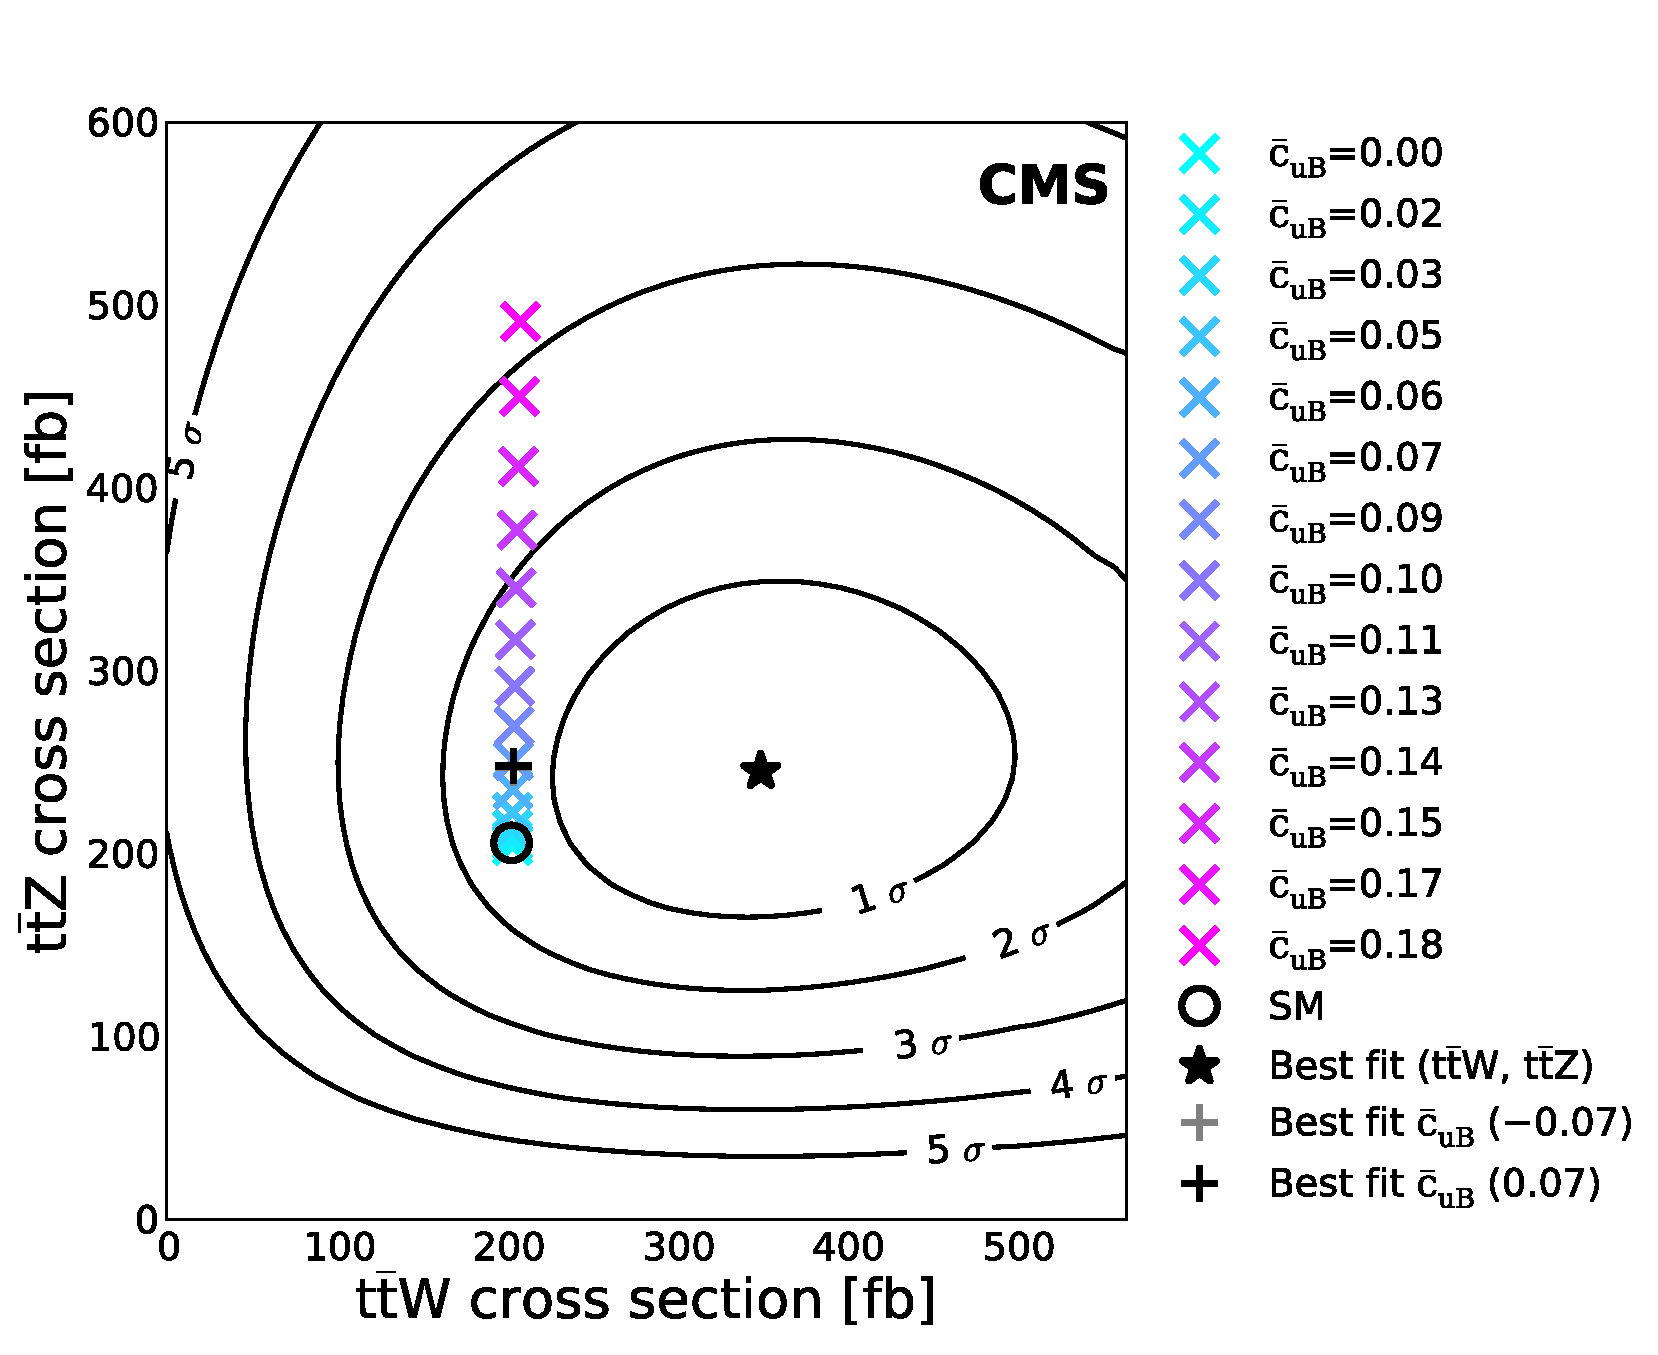
\includegraphics[width=\textwidth]{figures/eight-TeV/NP/operator_points_color_cycled_cuB_ttZ_ttW_2d_v4_mod_print}
    \caption{}
  \end{subfigure}%
  \begin{subfigure}{0.5\textwidth}
    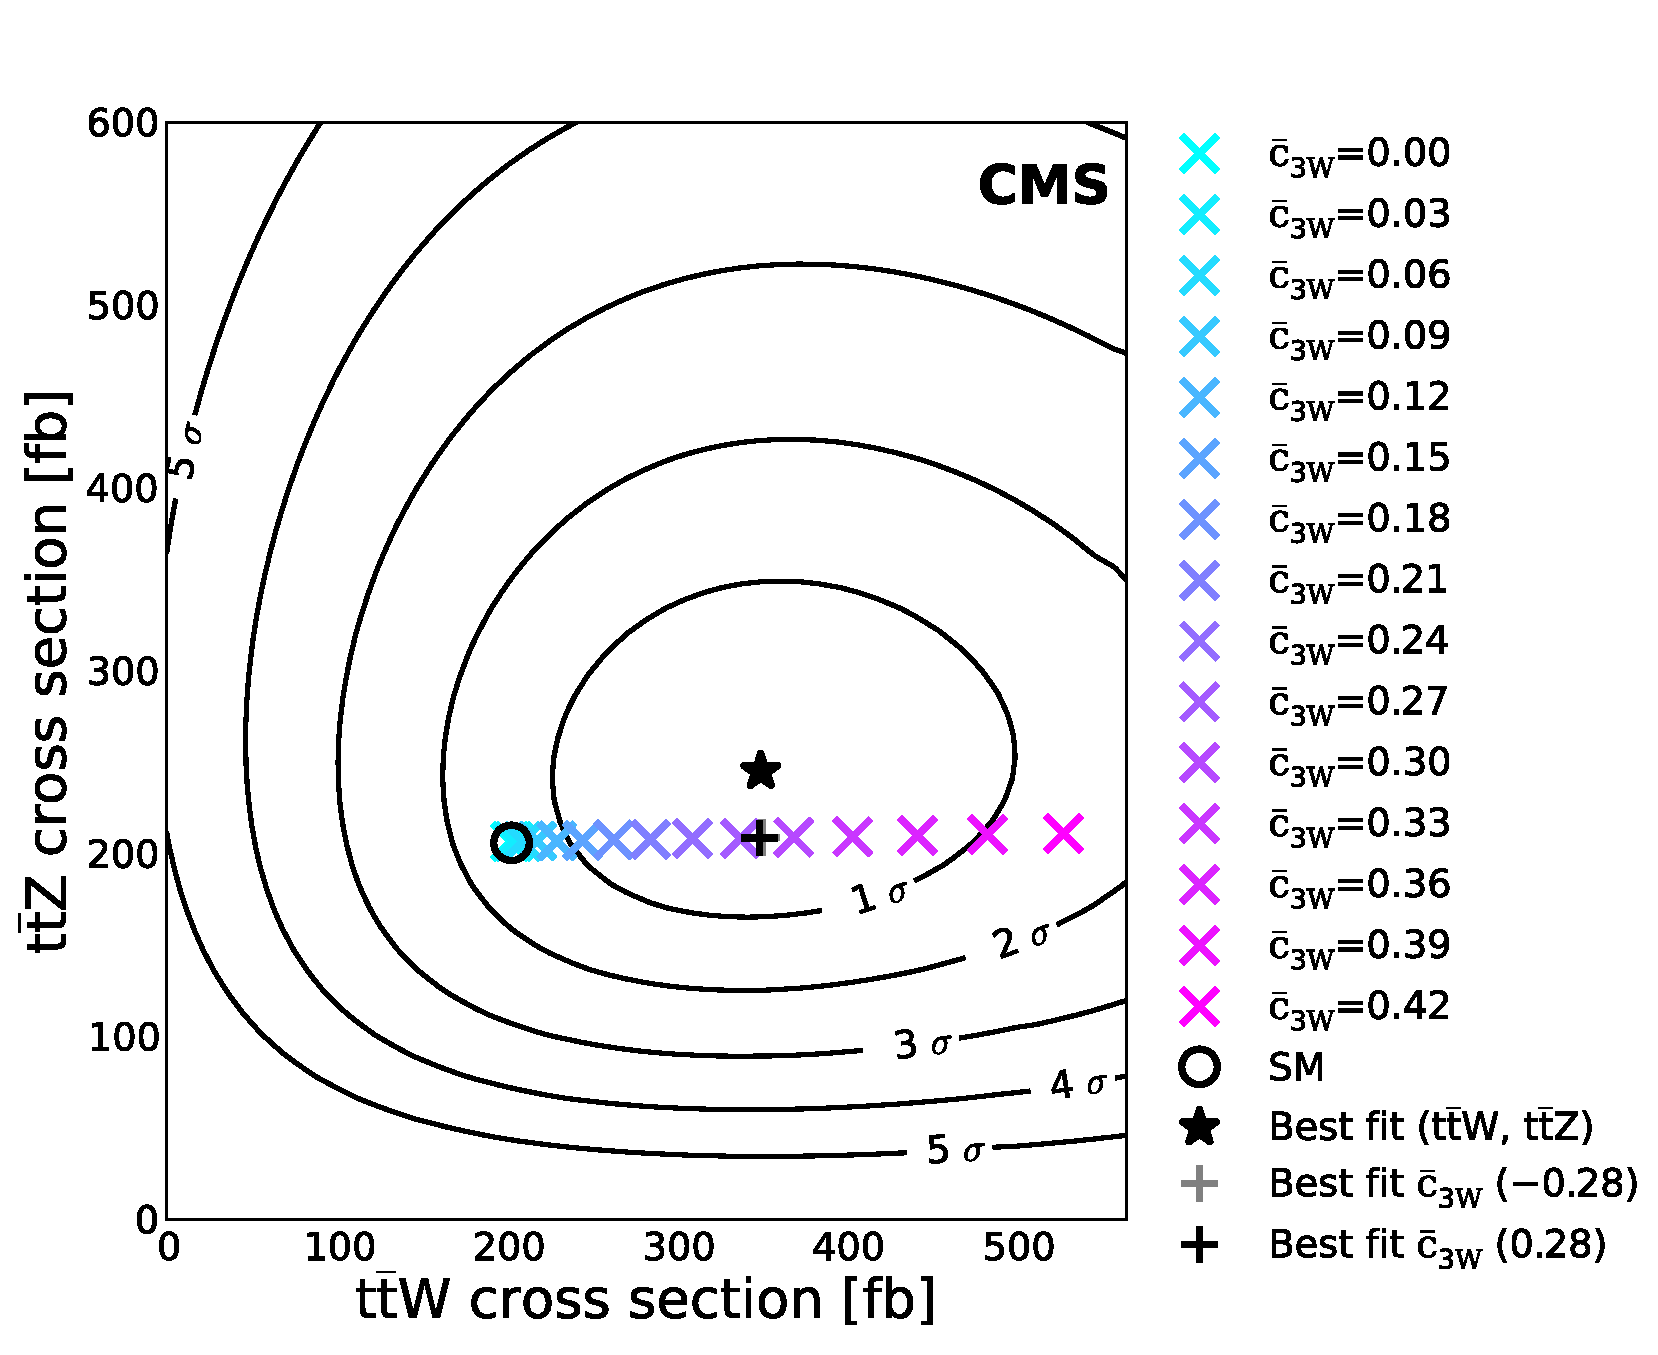
\includegraphics[width=\textwidth]{figures/eight-TeV/NP/operator_points_color_cycled_c3W_ttZ_ttW_2d_v4_mod_print}
    \caption{}
  \end{subfigure}
  \begin{subfigure}{0.5\textwidth}
    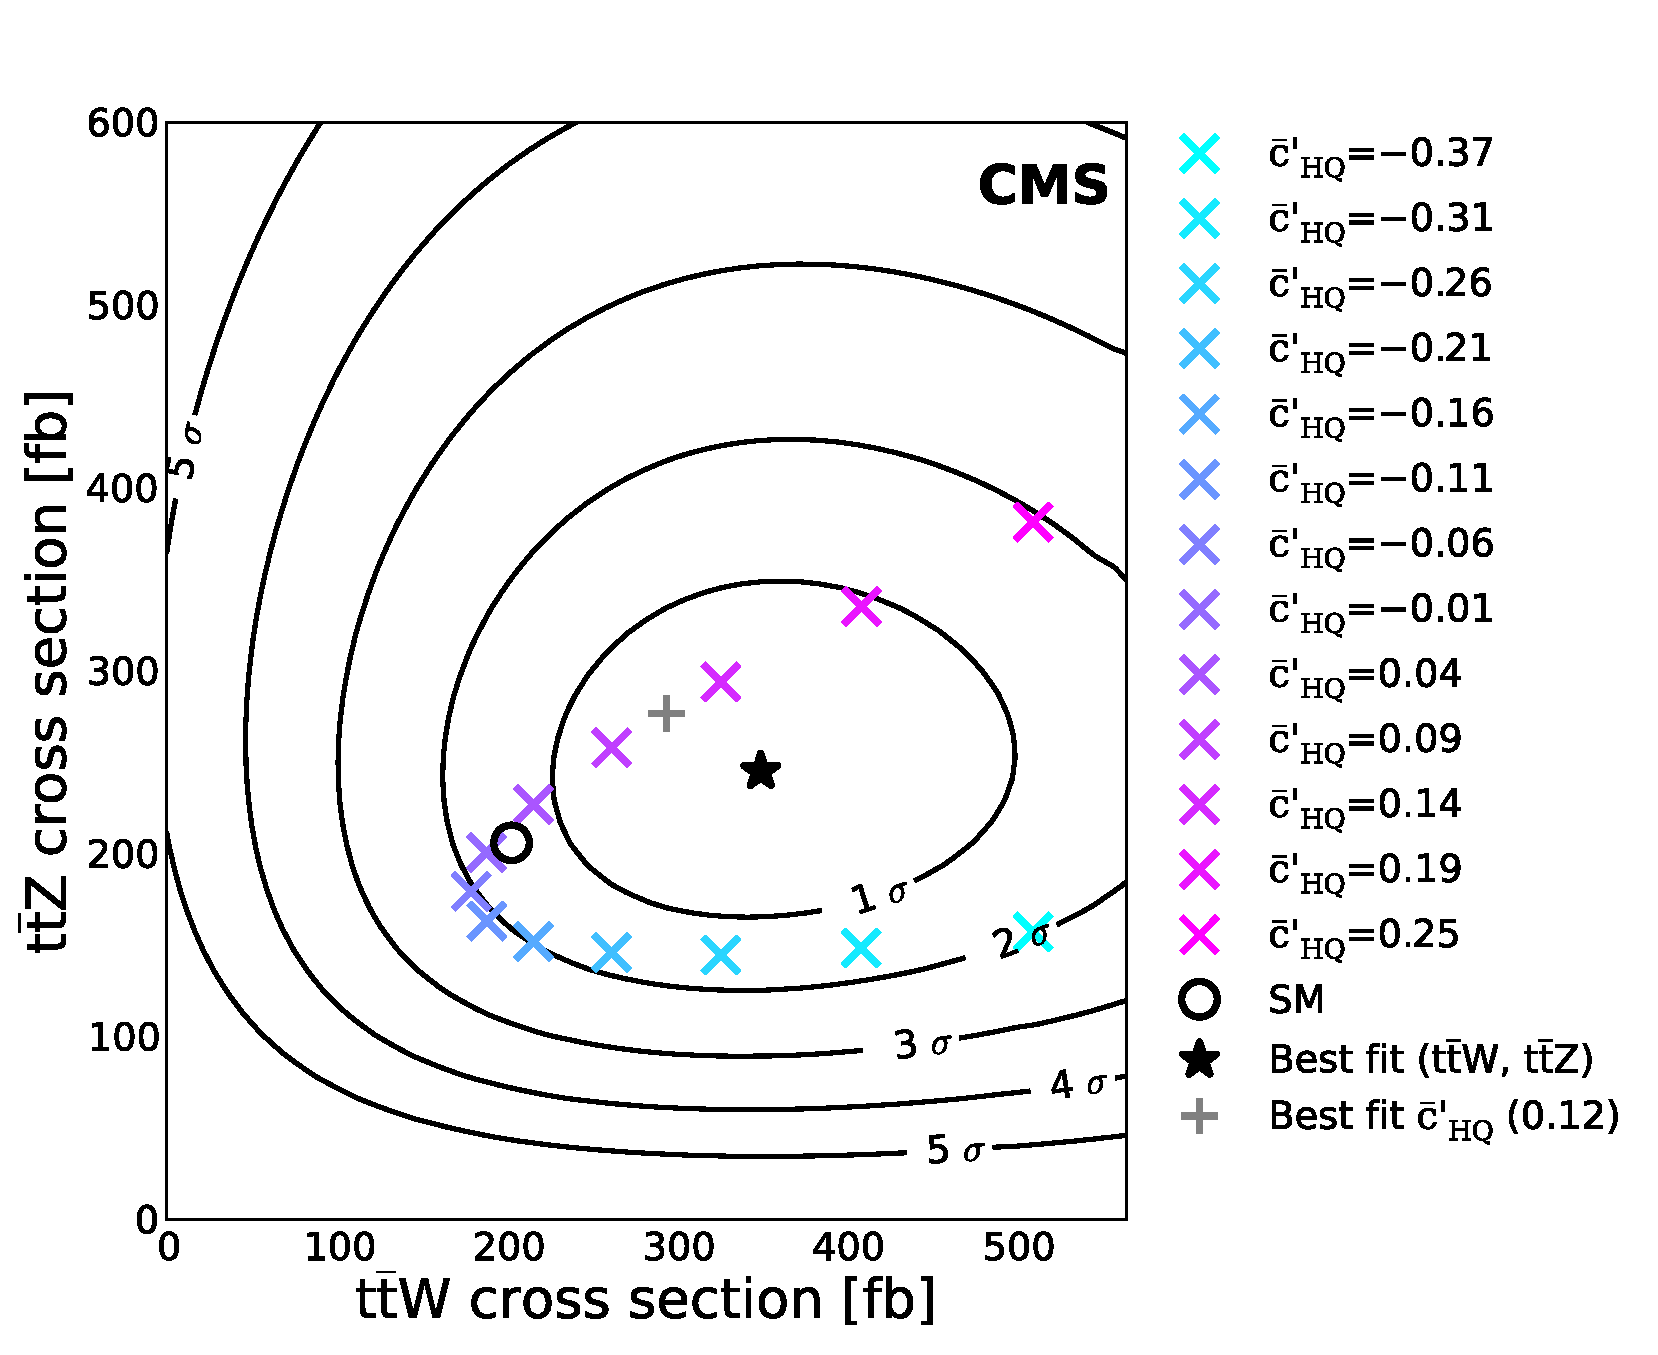
\includegraphics[width=\textwidth]{figures/eight-TeV/NP/operator_points_color_cycled_cpHQ_ttZ_ttW_2d_v4_mod_print}
    \caption{}
  \end{subfigure}%
  \begin{subfigure}{0.5\textwidth}
    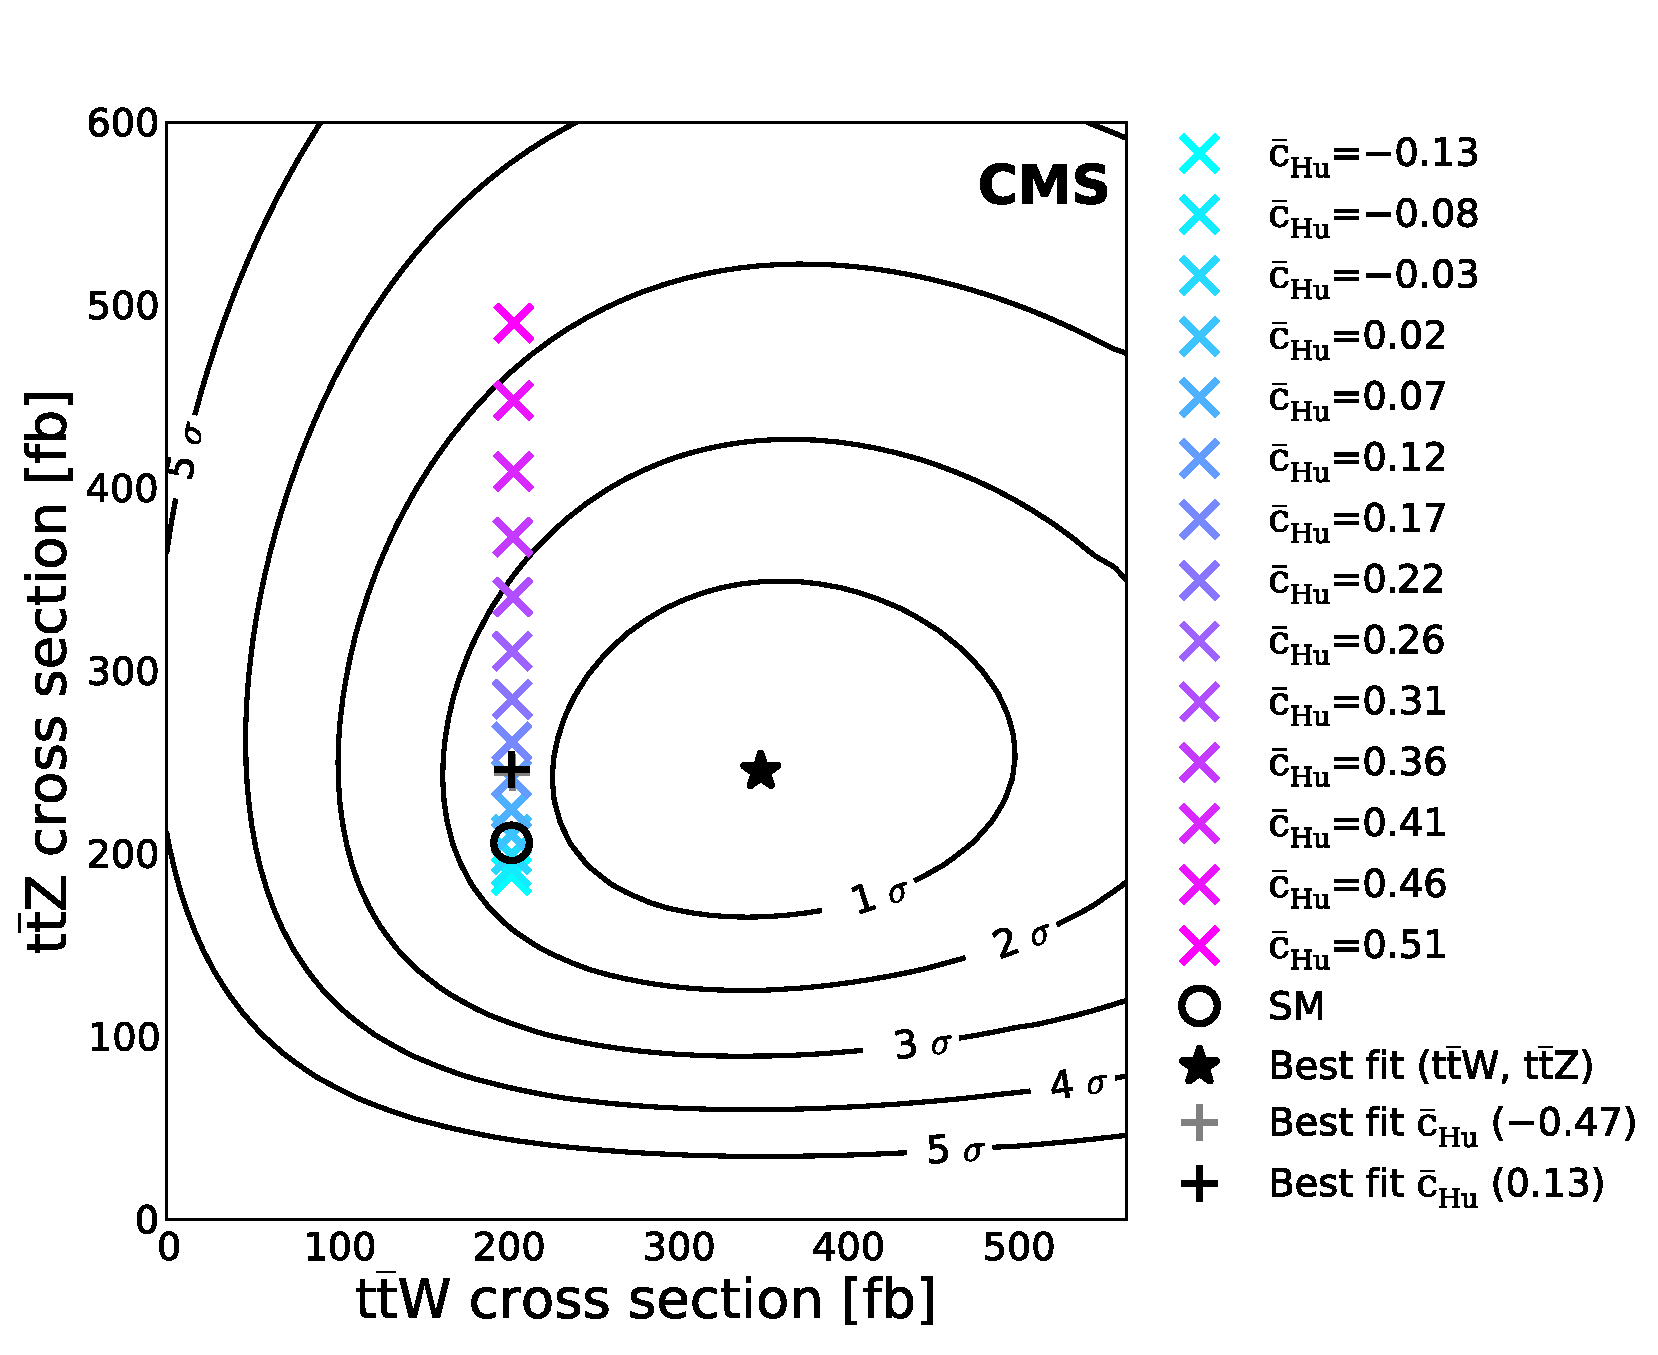
\includegraphics[width=\textwidth]{figures/eight-TeV/NP/operator_points_color_cycled_cHu_ttZ_ttW_2d_v4_mod_print}
    \caption{}
  \end{subfigure}
  \begin{subfigure}{0.5\textwidth}
    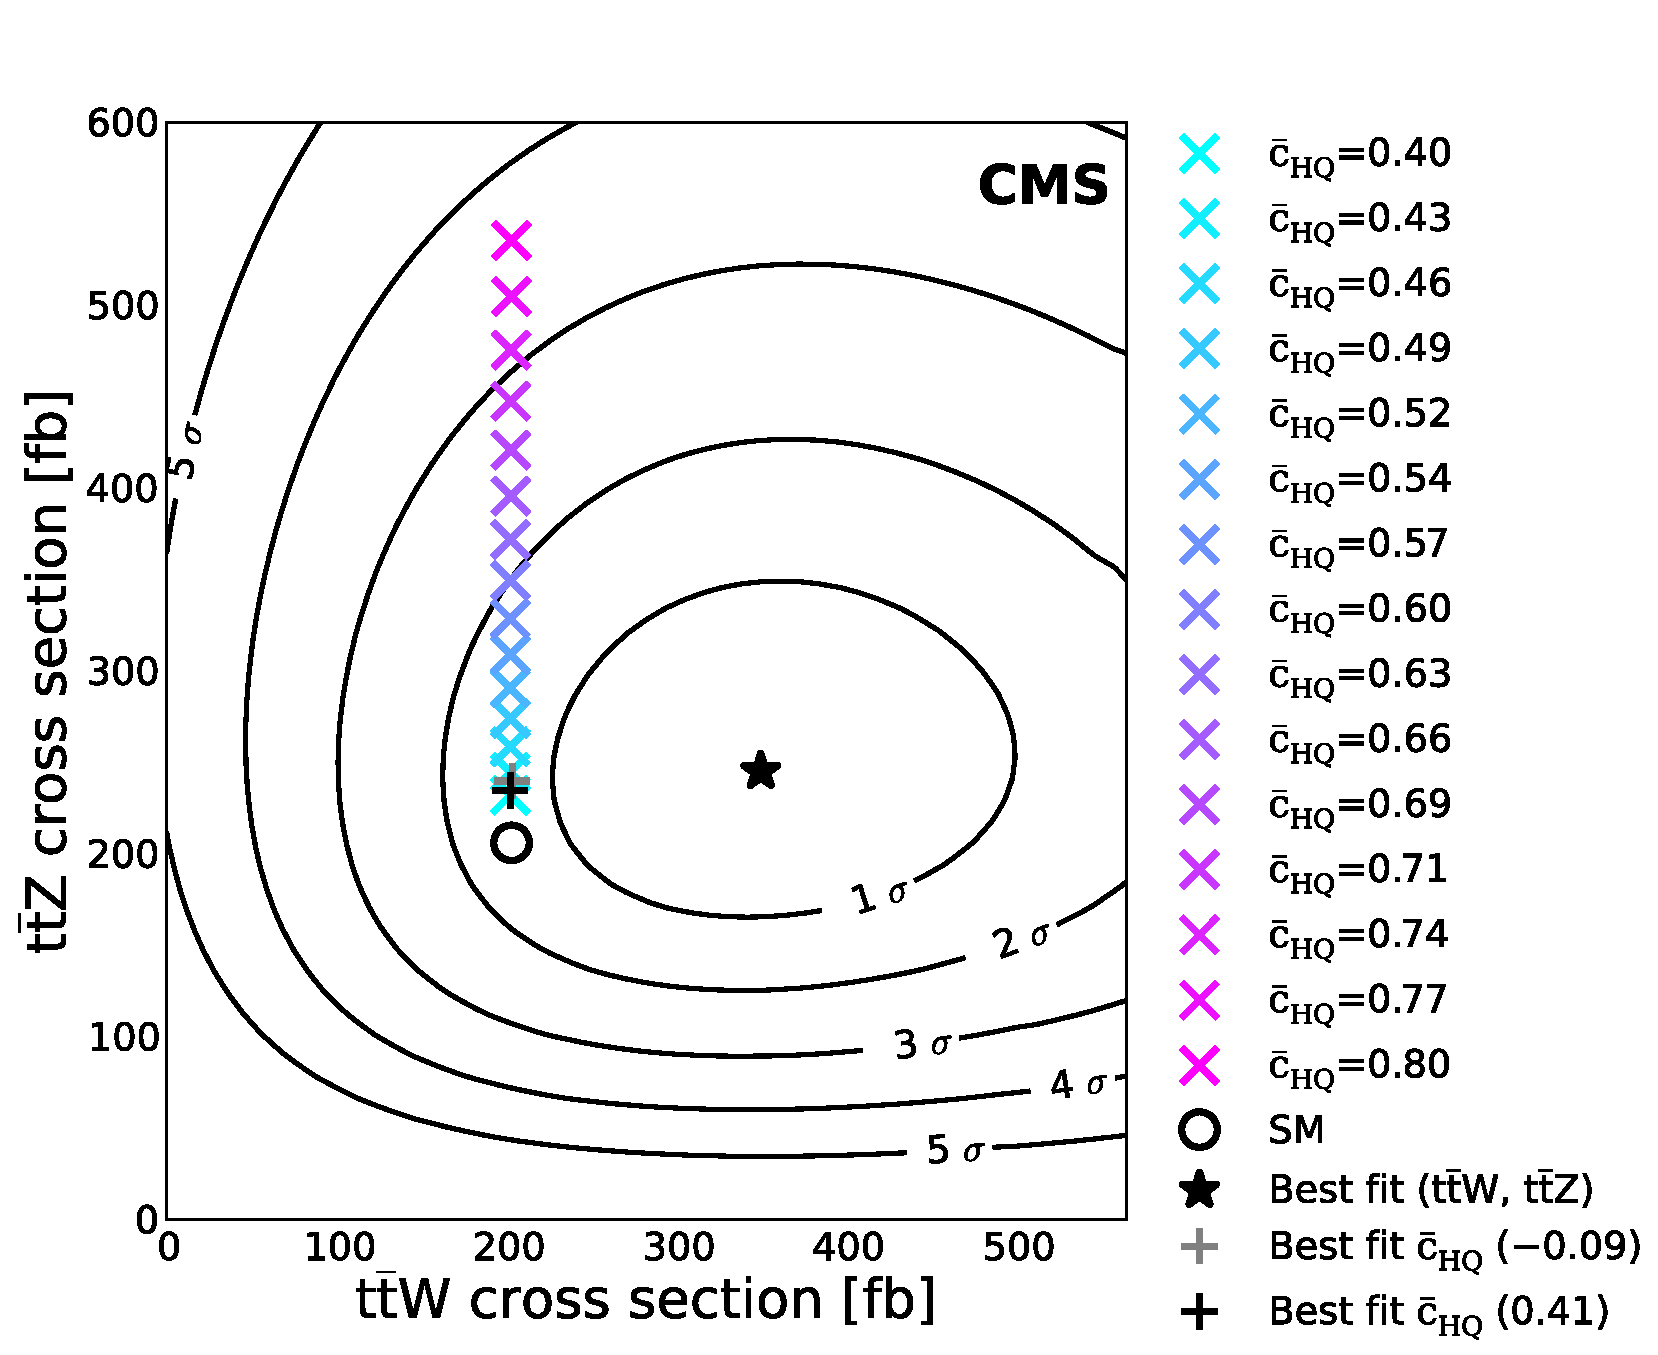
\includegraphics[width=\textwidth]{figures/eight-TeV/NP/operator_points_color_cycled_cHQ_ttZ_ttW_2d_v4_mod_print}
    \caption{}
  \end{subfigure}
  \vspace{-1cm}
  \caption[Best fit values in the $\sigma_{\ttW}$, $\sigma_{\ttZ}$ plane (\eightTeV)]{Sampled coefficient values (crosses) and best fit value (plus signs) for \cuB (a), \cthreeW (b), \cpHQ (c), \cHu (d), and \cHQ (e), plotted in the $\sigma_{\ttW}$, $\sigma_{\ttZ}$ plane, for the \eightTeV analysis. The simultaneous best fit to $\mu_{\ttW}$ and $\mu_{ttZ}$ is shown as a star.}
  \label{fig:8-2d}
\end{figure}

\begin{figure}[!htb]
  \begin{subfigure}{0.5\textwidth}
    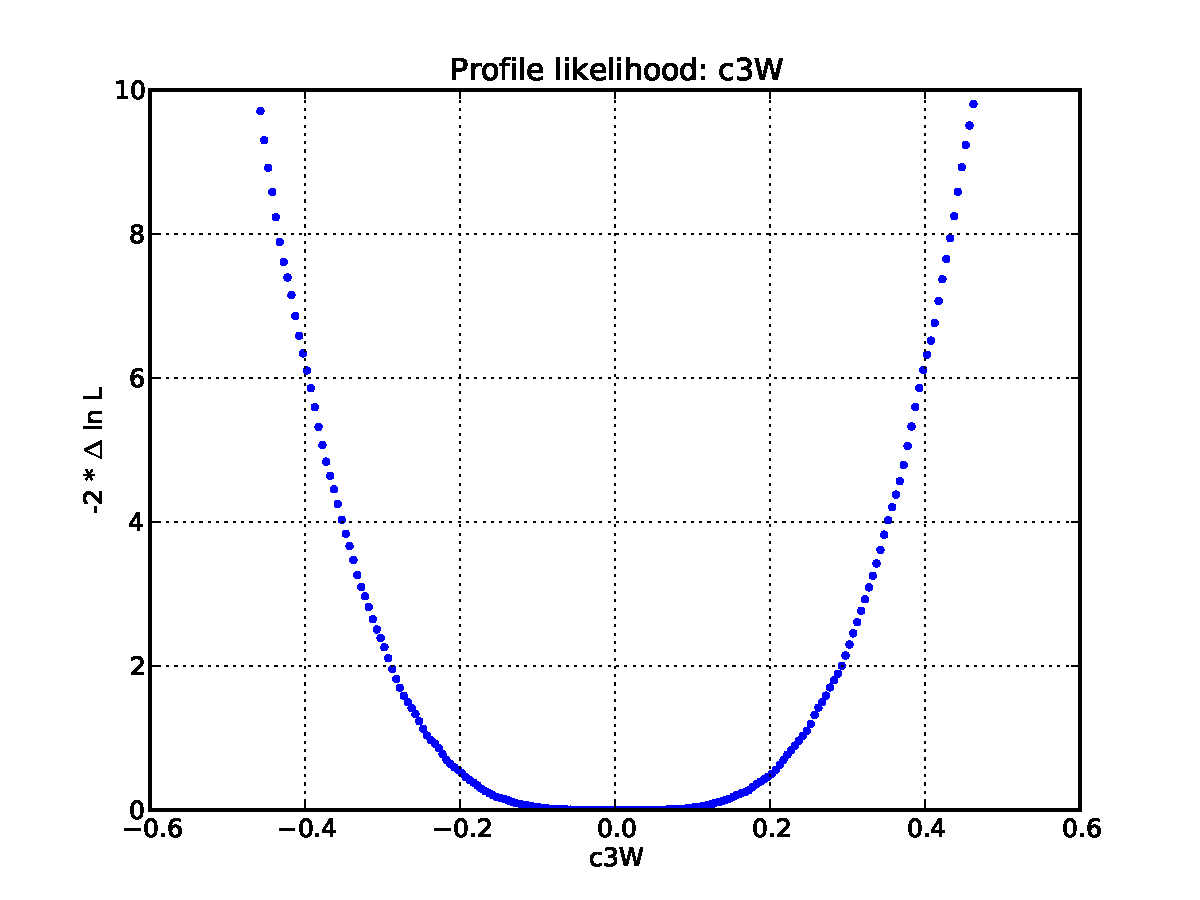
\includegraphics[width=\textwidth]{figures/eight-TeV/NP/c3W_NLL}
    \caption{}
  \end{subfigure}%
  \begin{subfigure}{0.5\textwidth}
    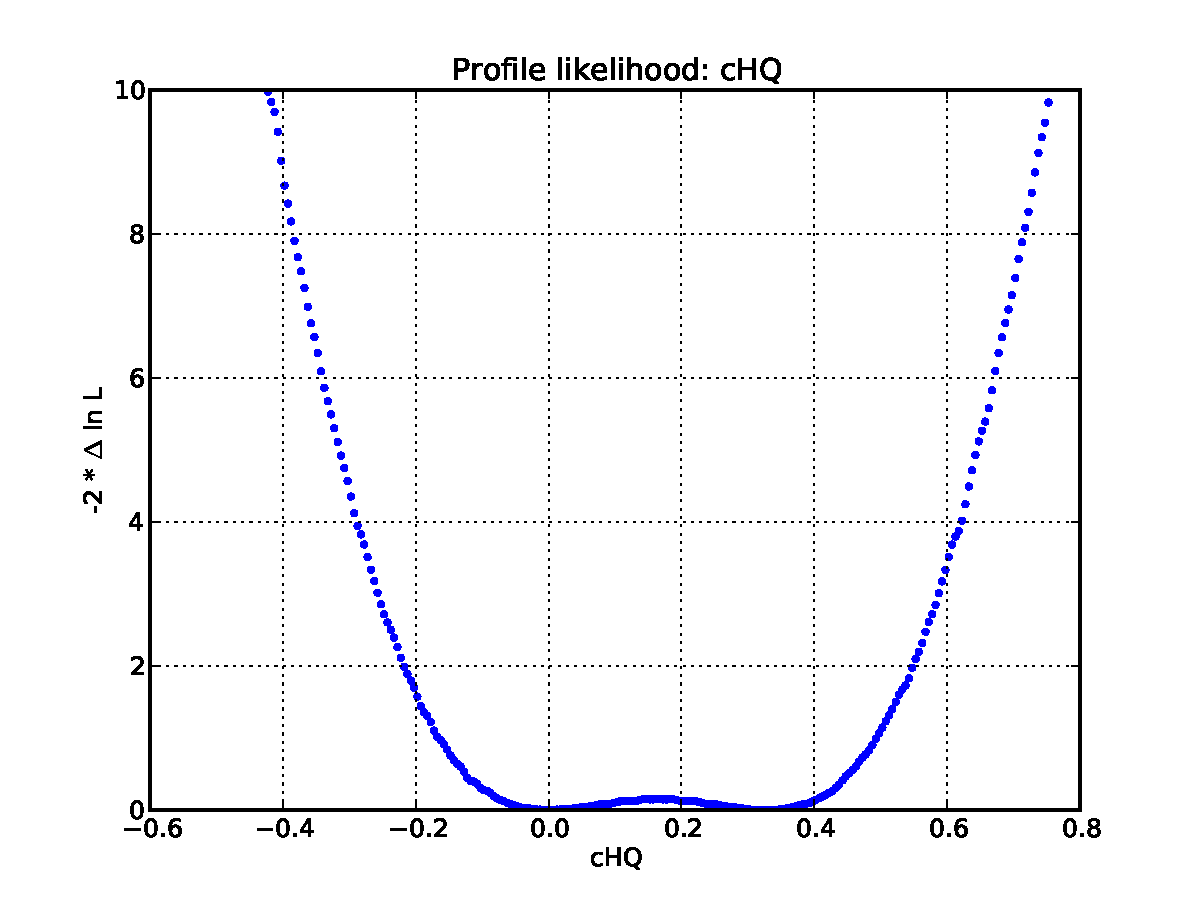
\includegraphics[width=\textwidth]{figures/eight-TeV/NP/cHQ_NLL}
    \caption{}
  \end{subfigure}
  \begin{subfigure}{0.5\textwidth}
    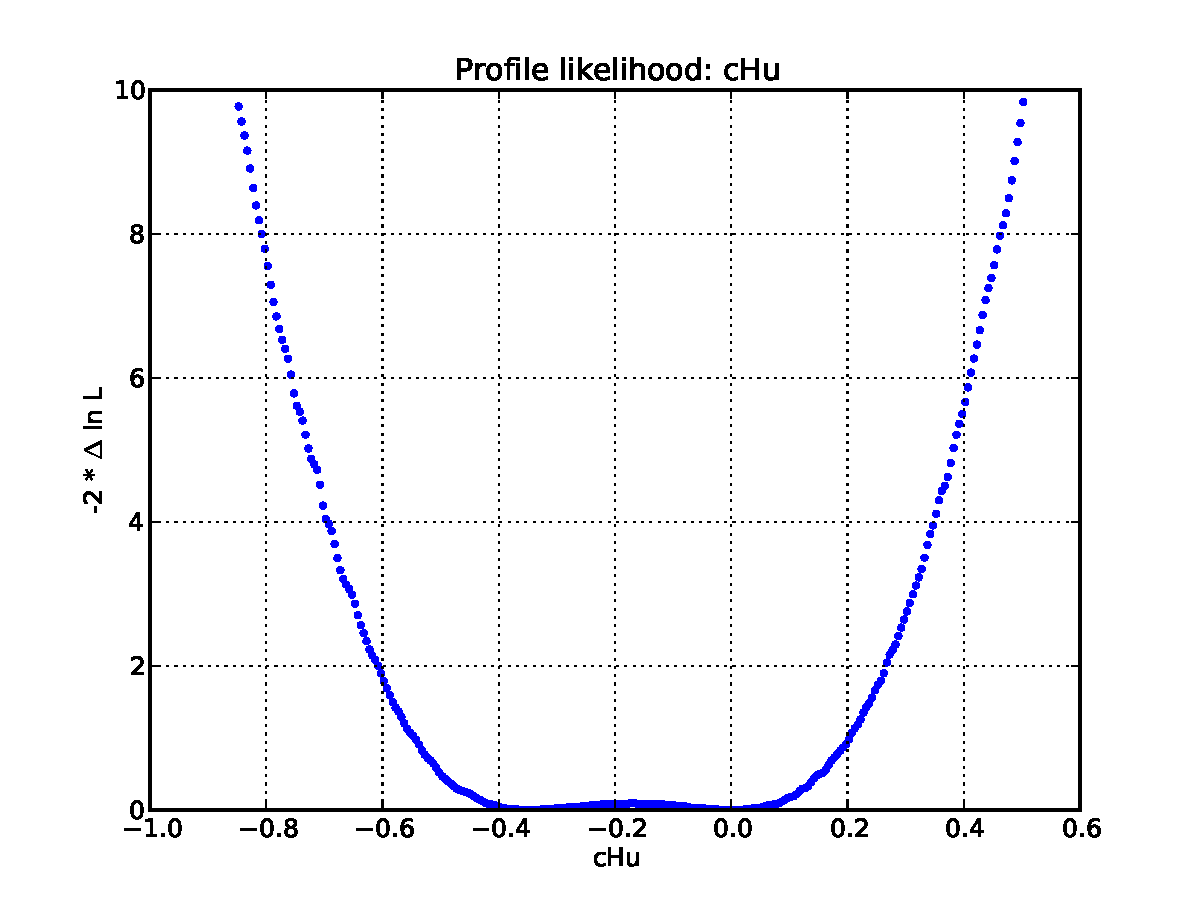
\includegraphics[width=\textwidth]{figures/eight-TeV/NP/cHu_NLL}
    \caption{}
  \end{subfigure}%
  \begin{subfigure}{0.5\textwidth}
    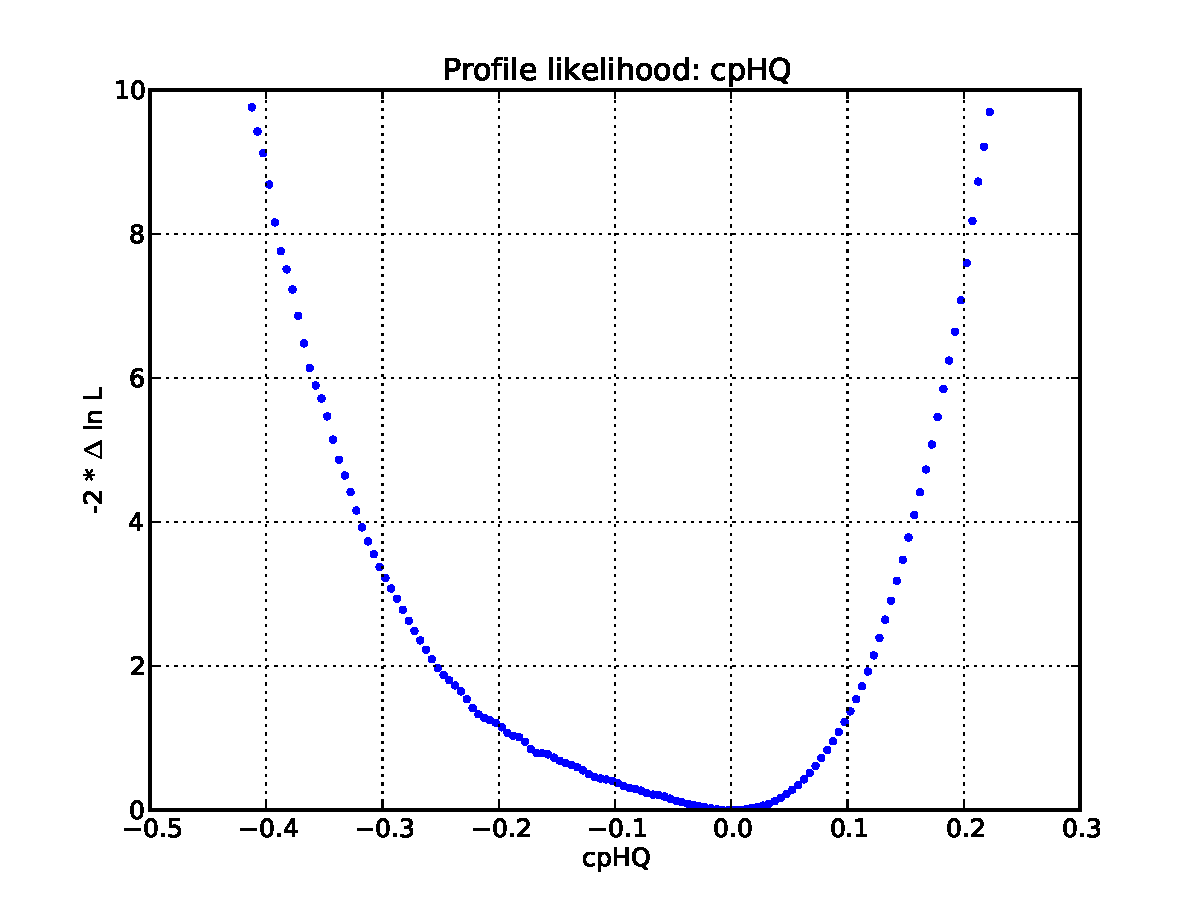
\includegraphics[width=\textwidth]{figures/eight-TeV/NP/cpHQ_NLL}
    \caption{}
  \end{subfigure}
  \begin{subfigure}{0.5\textwidth}
    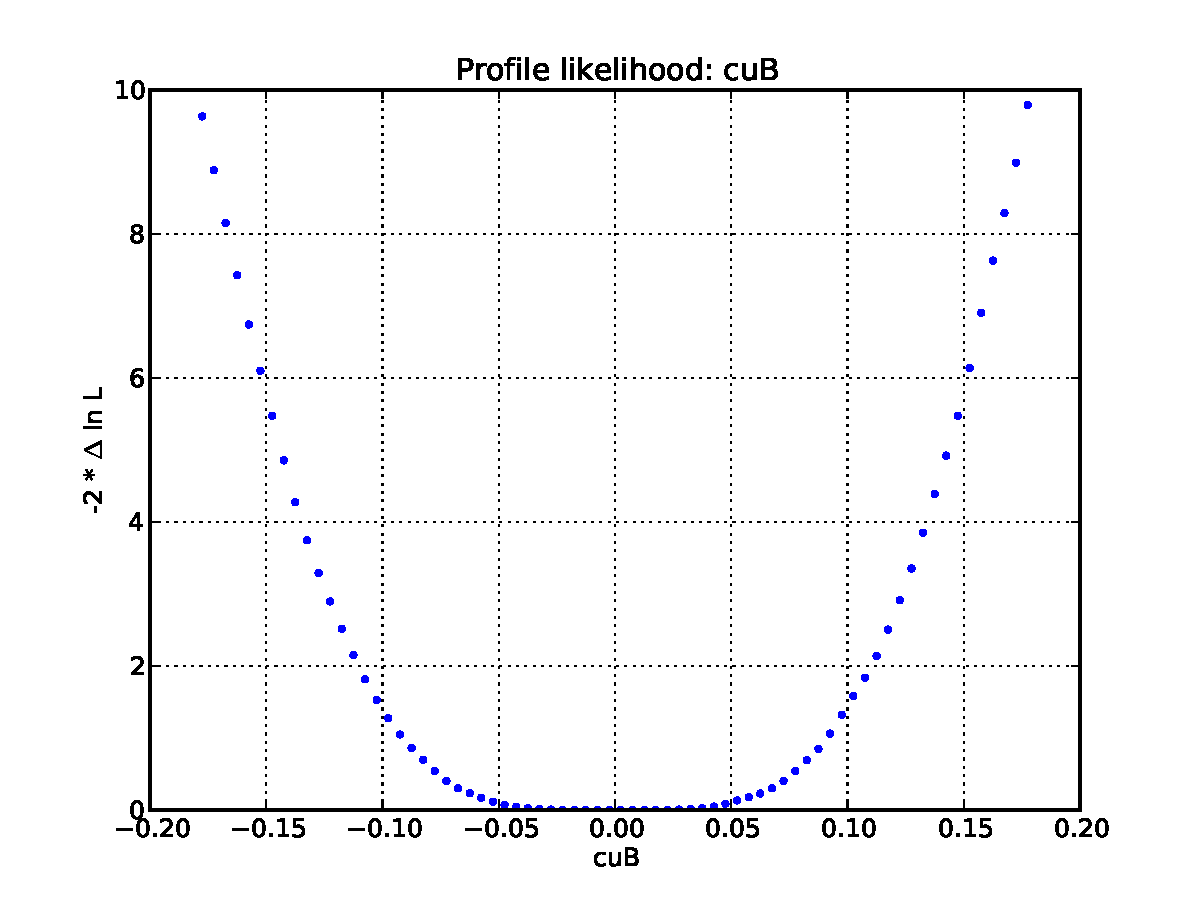
\includegraphics[width=\textwidth]{figures/eight-TeV/NP/cuB_NLL}
    \caption{}
  \end{subfigure}
  \caption[Profile likelihood scans (\eightTeV)]{Profile likelihood scans for \cthreeW (a), \cHQ (b), \cpHQ (c), \cuB (d), and \cHu (e) for the \eightTeV analysis.}
  \label{fig:8-nll}
\end{figure}
\todo{best fit vs best-fit}

Each coupling was scanned with all other couplings set to their SM value.
Profile likelihood scans are shown in~\cref{fig:8-nll}. Best fit values, along
with $1\sigma$ and $2\sigma$ CL ranges, are summarized
in~\cref{tab:8-constraints}. Operators for which the minima in $\mu_{\ttZ}(c_1)$
and $\mu_{\ttW}(c_1)$ coincide have symmetric likelihood distributions because
the cross section scaling as a function of the Wilson coefficient is quadratic;
thus, there are two coefficient values corresponding to the same scaling.

\begin{landscape}
  \begin{table}
    \centering
    \caption{Constraints on selected Wilson coefficients (\eightTeV)}
    \label{tab:8-constraints}
    \input{tables/eight-TeV/constraints}
  \end{table}
\end{landscape}

\section{\thirteenTeV analysis}
\label{sec:13-eft}
Building on the work described in~\cref{sec:8-eft}, the \thirteenTeV data
described in~\cref{chap:13-TeV} was re-interpreted within the framework of EFT.
A strategy similar to that used for the \eightTeV analysis was employed, but
several improvements were incorporated.

\subsection{Independent constraints}
\label{ssec:13-1d-eft}
The \textsc{FeynRules} implementation from reference~\cite{Alloul2014} used in
the \SI{8}{TeV} analysis assumes flavor-independent fermion couplings. Because
the Z and W boson coupling to light quarks is highly constrained by other
measurements, we removed the couplings to the first two generations with help
from Martin~\cite{Martin2017}. For this reason, results from the \eightTeV
analysis and \thirteenTeV analysis cannot be directly compared. This modified
implementation was then used to determine $\mu(c_1)$, as described
in~\cref{ssec:eft-strategy}, again considering the NP effects of one operator at
a time. The strategy was more careful than what was used in the \eightTeV
analysis. If the \madgraph calculation were infinitely precise, only three
points would be required to completely specify the system of equations and
calculate the three structure constants exactly. We would then be free to choose
any three values when setting up the system of equations. Due to the finite
precision of the \madgraph calculation, however, care must be taken in choosing
the sample points: they should adequately cover the parameter space where the
fit will be evaluated. This approach prevents noise in the sampled region from
having a disproportionate effect in the regions to which the fit is
extrapolated. To choose which points to sample, a \emph{coarse scan} was first
run for each coefficient using \madgraph to evaluate the cross section at ten
points sampled using a pseudo-random number generator in the interval $-4\pi <
c_1 < 4\pi$. These points were then divided by $\sigma_\text{SM}$ and fit with a
quadratic function to determine $\mu_\text{coarse}(c_1)$. Next, 30 values of
$c_1$ were sampled using a pseudo-random number generator in the range
corresponding to $\mu_\text{coarse}(c_1) < 10$, and a quadratic fit to these
points was used to determine $\mu(c_1)$. This strategy was found to improve the
quality of the fit. Next, we used $\mu(c_1)$ to construct a profile likelihood
test statistic in terms of $c_1$. The likelihood was then maximized using the
Higgs Combine tool to find the best fit $c_1$ for the 39 Wilson coefficients
included in the \textsc{FeynRules} model. Each coupling was scanned with all
other couplings set to their SM values.

In the \eightTeV analysis, only the scaling of \ttW and \ttZ due to NP effects
was included. In the \thirteenTeV analysis, the NP effects on \ttH were
considered as well because \ttH is a sizable and irreducible background to \ttW,
and many operators produce similar cross section scaling of both processes.

The strategy used to select which operators to study was also more sophisticated
in the \thirteenTeV analysis. First, we eliminated any operators that did not
affect \ttW, \ttZ, or \ttH. To determine which operators to discard, we fit
$\sigma(c_1) = s_0 + s_1 c_1 + s_2c_1^2$ and eliminated operators where $s_1$
and $s_2$ were both less than $10^{-5}$. This requirement excluded the operators
proportional to the following Wilson coefficients: $\bar{c}_\text{l}$,
$\bar{c}_\text{lB}$, $\bar{c}_\text{d}$, $\bar{c}_\text{2B}$,
$\bar{c}_\text{lW}$, $\bar{c}_\text{dB}$, and $\bar{c}_\text{dW}$.

We also eliminated operators with strong effects on already very precisely
measured processes such as \ttbar production, because significant deviations
would have been apparent from previous measurements. We defined the extreme
signal scaling $\mu_\text{e}(c_1)$ to be $\mu(c_1)$ evaluated at the $c_1$ which
that $\abs{\mu(c_1) - 1}$, the deviation from the SM, within the range of $c_1$
corresponding to $2\sigma$ sensitivity. Operators producing $\abs{\mu_\text{e} -
1} > 0.7$ for $\ttbar$, inclusive Higgs, WW, and WZ were excluded. The
$\mu_\text{e}(c_1)$ values for all operators that satisfied the requirement for
$s_1$ and $s_2$ but failed to meet the requirement on $\mu_\text{e}(c_1)$ are
presented in~\cref{tab:mu-ext-mu-ext-fail}.

\todo{add cHQ}
\begin{table}
  \centering
  \input{tables/thirteen-TeV/mu-ext-mu-ext-fail}
\end{table}

Sixteen operators satisfied all the requirements on sensitivity and
$\mu_\text{e}$: \cuW, \cH, \tcthreeG, \cthreeG, \cuG, \cHu, \ctwoG, \cuB, \cHB,
\tcHW, \cHud, \cHQ, \cB, \tcA, \cpHQ, and \cu. For each of these operators, we
estimated the effect of NP on yields by scaling the yields for each process by
$\mu_\text{e}(c_1)$. Because the nonprompt background is dominated by \ttbar, we
used $\mu_\text{e, \ttbar}$ to estimate the impact of NP effects on that
background. For rare backgrounds, we made the simplifying assumption that the
baseline yields were due to equal contributions from WZZ, ZZZ, WWW, and WWZ.
\Cref{tab:mu-ext-yield-fail} summarizes the $\mu_\text{e}$ due to operators that
had significant effects on background yields, mainly due to the tqZ, tHq, VH (WH
or ZH), and triboson processes. The corresponding difference in yields due to
these operators is tabulated in~\cref{tab:yield-yield-fail}. These operators
were excluded from further study. \Cref{tab:mu-ext-yield-pass} and
\cref{tab:yield-yield-pass} summarize the  $\mu_\text{e}(c_1)$ and yields,
respectively, due to operators for which the effect on background yields was
considered acceptably small. The operators that were excluded by each
requirement are summarized in table~\cref{tab:elimination}. Eight operators
satisfied all requirements: \cH, \tcthreeG, \cthreeG, \cuG, \cuB, \cHu, \cuW,
and \ctwoG. % FIXME Feynman diagrams representing the largest LO contributions
for the process with the most significant NP effects due to each operator are
shown in~\cref{fig:diagrams}.


% FIXME use S tables everywhere
% see  ~/www/.private/ttV/45/1/2
% todo: include appendix with per-channel yields?
% todo: label 8 tev vs 13 tev everywhere
\begin{landscape}
  \begin{table}
    \input{tables/thirteen-TeV/mu-ext-yield-fail}
  \end{table}
  \begin{table}
    \input{tables/thirteen-TeV/mu-ext-yield-pass}
  \end{table}
  \begin{table}
    \input{tables/thirteen-TeV/yield-yield-fail}
  \end{table}
  \begin{table}
    \input{tables/thirteen-TeV/yield-yield-pass}
  \end{table}
\end{landscape}

\begin{table}
  \input{tables/thirteen-TeV/elimination}
\end{table}

To obtain $\sigma(c_1)$ from the post-fit values of the Wilson coefficients and
nuisance parameters, we used the following transformation:
\begin{equation}
  \sigma(c_1) = \sigma_\mathrm{NLO} \cdot \mu(c_1) \cdot \kappa_j^{\theta_j},
\end{equation}
where $\theta_j$ corresponds to the post-fit nuisance parameters due to the
scale and PDF uncertainties. These nuisances were parameterized by using a
log-normal probability density function characterized by $\kappa_j > 1$, which
encodes the spread in the distribution, with ($\kappa_j - 1$) corresponding
roughly to the relative uncertainty~\cite{Cousins2010}. To determine the
$1\sigma$ and $2\sigma$ contours in the $\sigma_{\ttZ}/\sigma_{\ttW}$ plane, we
sampled the parameters randomly from the post-fit covariance matrix, then drew
contours containing \SI{68.27}{\percent} and \SI{95.45}{\percent} of the
samples. The result is presented in the right panels
of~\cref{fig:results-cuG,fig:results-cuW,fig:results-c3G,fig:results-tc3G,fig:results-c2G,fig:results-cuB,fig:results-cH,fig:results-cHu}.
The likelihood scans are presented in the center panels
of~\cref{fig:results-cuG,fig:results-cuW,fig:results-c3G,fig:results-tc3G,fig:results-c2G,fig:results-cuB,fig:results-cH,fig:results-cHu}.
We removed any assumptions about the energy scale of the NP made in
reference~\cite{Alloul2014} and report the ratio $c_i/\Lambda^2$. In cases in
which $\sigma_{\text{SM+NP}}(c_i)$ had the same minimum for all three processes,
the profile likelihood was symmetric around this point, and we present the
results for $|c_i - c_{i,\text{min}}|$ to make this symmetry explicit.

The scaling due to NP effects, evaluated at the best fit value of the Wilson
coefficient for \ttZ, \ttW, and \ttH, is tabulated in~\cref{tab:scaling}.
In~\cref{fig:ratio-cuG-cuW,fig:ratio-c3G-tc3G,fig:ratio-c2G-cuB,fig:ratio-cH-cHu},
the ratio between the yields resulting from a fit with two free parameters for
$\mu_{\ttZ}$ and $\mu_{\ttW}$ and the yields resulting from the fit with one
free parameter for $c_1$, which was subject to the constraints of
$\mu_{\ttZ}(c_1)$, $\mu_{\ttW}(c_1)$, and $\mu_{\ttH}(c_1)$, is shown for each
coefficient. The small variations between categories can be explained by slight
differences in the best fit nuisance parameters. For \cuW and \cuG, which are
proportional to operators that affect all three processes, the observed excess
was accommodated reasonably well in both the \ttZ and \ttW channels. It is
evident (see~\cref{fig:ratio-cuG-cuW}) that the sensitivity was driven by the
\ttZ channel because in both cases, the ratio of the yields was approximately
one for \ttZ and \numrange{0.91}{0.95} for \ttW. This indicates that the fit was
more sensitive to the \ttZ channel and thus matched it more closely than the
\ttW channel. For the operators that are proportional to \tcthreeG, \cthreeG,
\cuB, and \ctwoG, which affect the \ttZ and \ttH processes but not the \ttW
process, the one-dimensional (1D) fit again yielded a coefficient value that
produced the same \ttZ scaling as in the two-dimensional (2D) fit. This result
is shown in the corresponding right panels
of~\cref{fig:results-c3G,fig:results-tc3G,fig:results-c2G,fig:results-cuB},
where the 1D best fit in the $\sigma_{\ttZ}, \sigma_{\ttW}$ plane agrees closely
with 2D best fit. The \ttH yield was higher due to the scaling of the \ttH
process, and the \ttW yield was lower because the \ttW process is not affected
by variations in this coefficient. Similarly, \cH only affects \ttH;
consequently, the ratios for both the \ttW and \ttZ channels are below one. The
\ttH ratio is also below one, although we expected the fit to yield a higher
scaling for \ttH as a substitute for \ttW. This effect was studied carefully; it
can be explained by a difference in the discriminant shapes of the \ttW and \ttH
channels, in combination with the higher sensitivity to the \ttZ channel. The
fit adjusted nuisance parameters to improve the agreement for the \ttZ channel
rather than scale the \ttH channel. The degree to which the nuisances affected
the fit can be seen in~\cref{fig:results-cH}; in the absence of nuisance
parameters, the 1D best fit cross would coincide with the theory point because
variations in \cH do not affect \ttW or \ttZ production. For \cHu, which only
affects \ttZ production, the best fit point matched the 2D case in the \ttZ
channel and was unable to accommodate the excess observed in the \ttW channel.

\begin{landscape}
  \begin{figure}
    \centering
    \resizebox{!}{7.2cm}{
        \includegraphics[height=\textheight]{figures/thirteen-TeV/NP/mu/cuG}\hspace{1cm}
        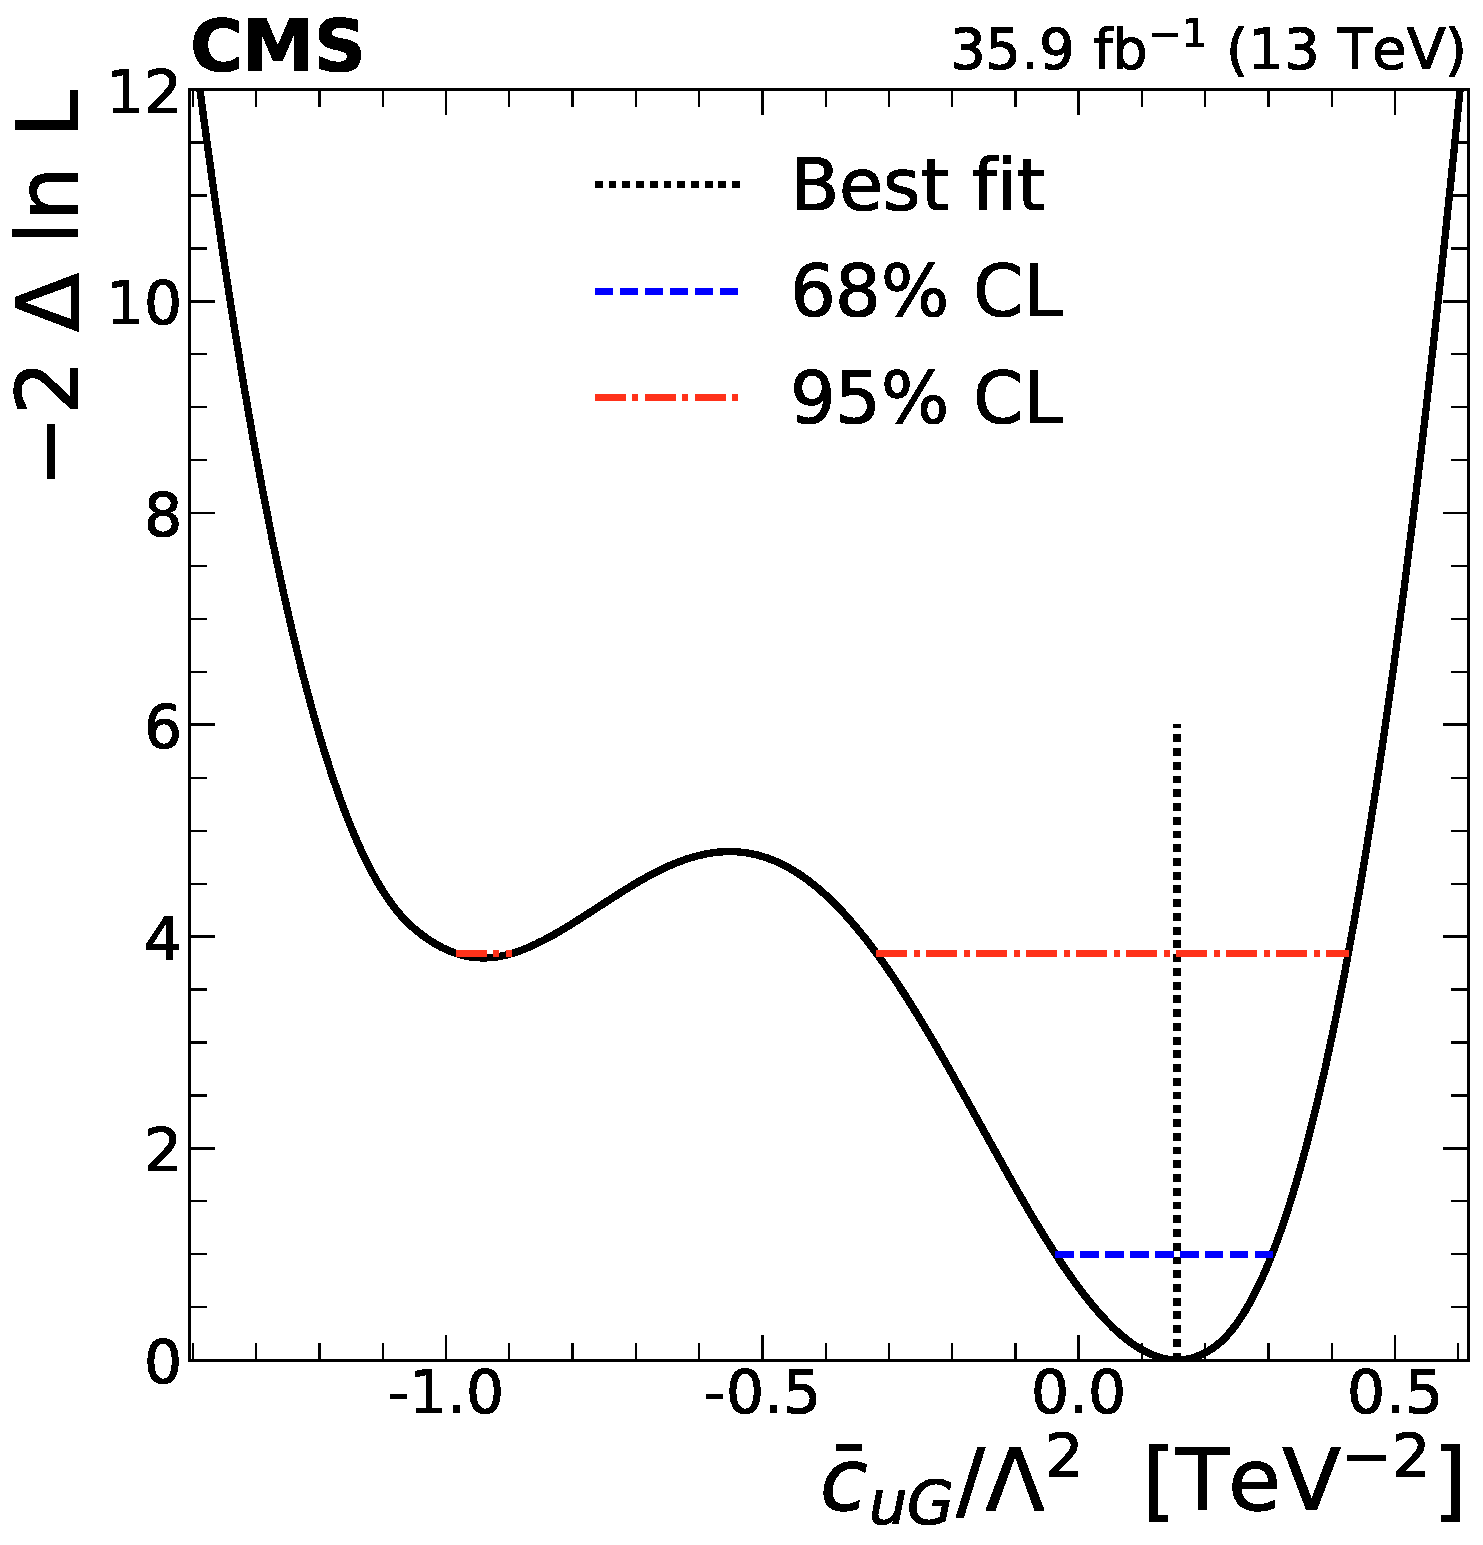
\includegraphics[height=\textheight]{figures/thirteen-TeV/NP/nll/cuG}\hspace{1cm}
        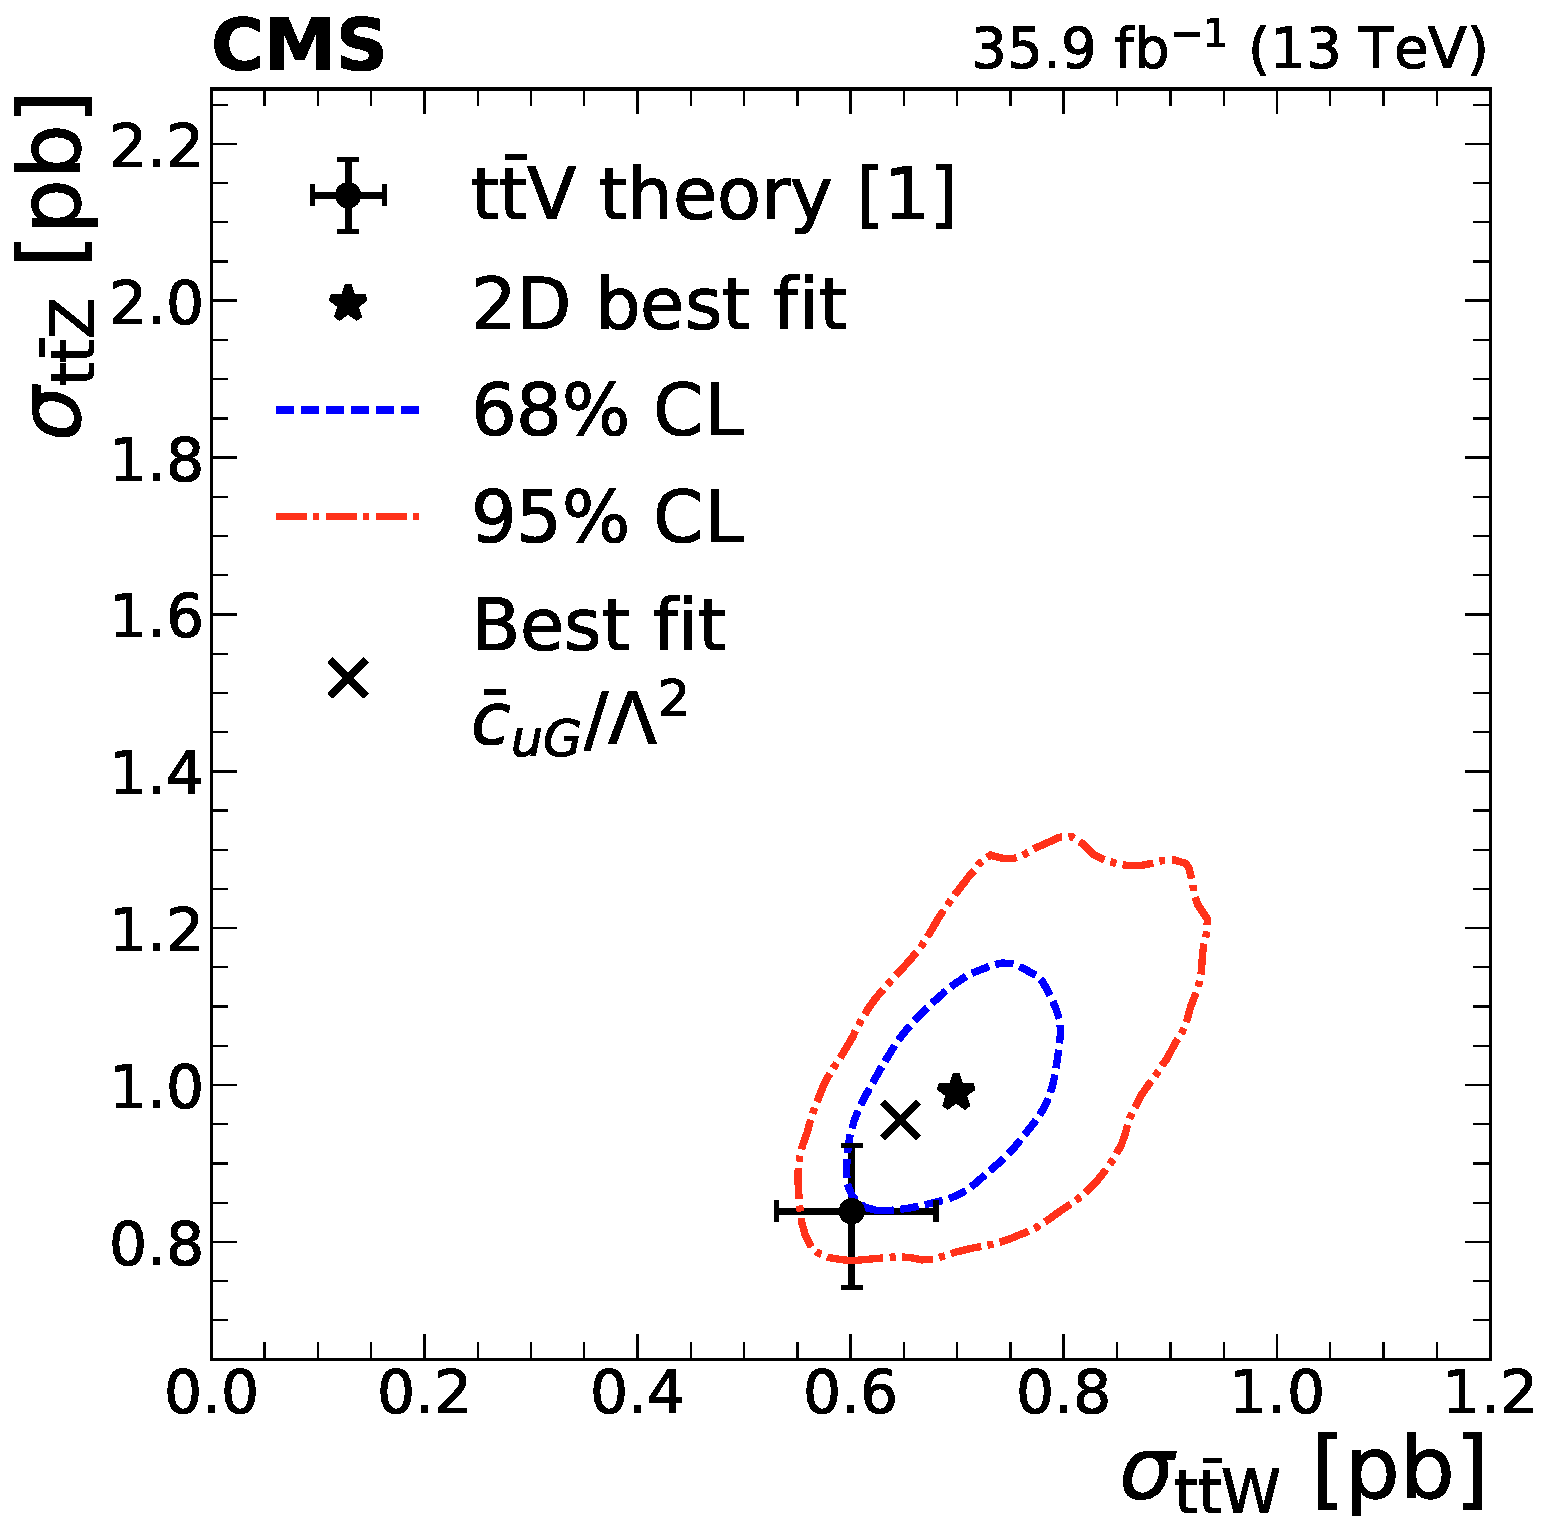
\includegraphics[height=\textheight]{figures/thirteen-TeV/NP/2D/ttZ_ttW_2D_1D_cuG}
      }
    \setlength{\capwidth}{14cm}
    \caption[Profile likelihood, $\mu(c_1)$, and best fit $c_1$ for \cuG (\thirteenTeV)]{Left: signal scaling as a function of the $c_1$ for \ttW (crosses), \ttZ (pluses), and \ttH (circles) for \cuG (\thirteenTeV analysis). Center: the test statistic $q(c_i)$ scan as a function of $c_1$, profiling all other nuisance parameters. The best fit value is indicated by a dotted line. Dashed and dash-dotted lines indicate \SI{68}{\percent} and \SI{95}{\percent} CL intervals, respectively. Right: The best fit $c_1$ value (shown as a cross), along with the corresponding \SI{68}{\percent} (dashed) and \SI{95}{\percent} (dash-dotted) contours in the $\sigma_{\ttZ}, \sigma_{\ttW}$ plane. The two-dimensional best fit to the \ttW and \ttZ cross sections is given by the star. The theory predictions~\cite{deFlorian:2016spz} are shown as a dot with bars representing their respective uncertainties.}%
    \label{fig:results-cuG}
  \end{figure}
  \begin{figure}
      \resizebox{!}{7.2cm}{
        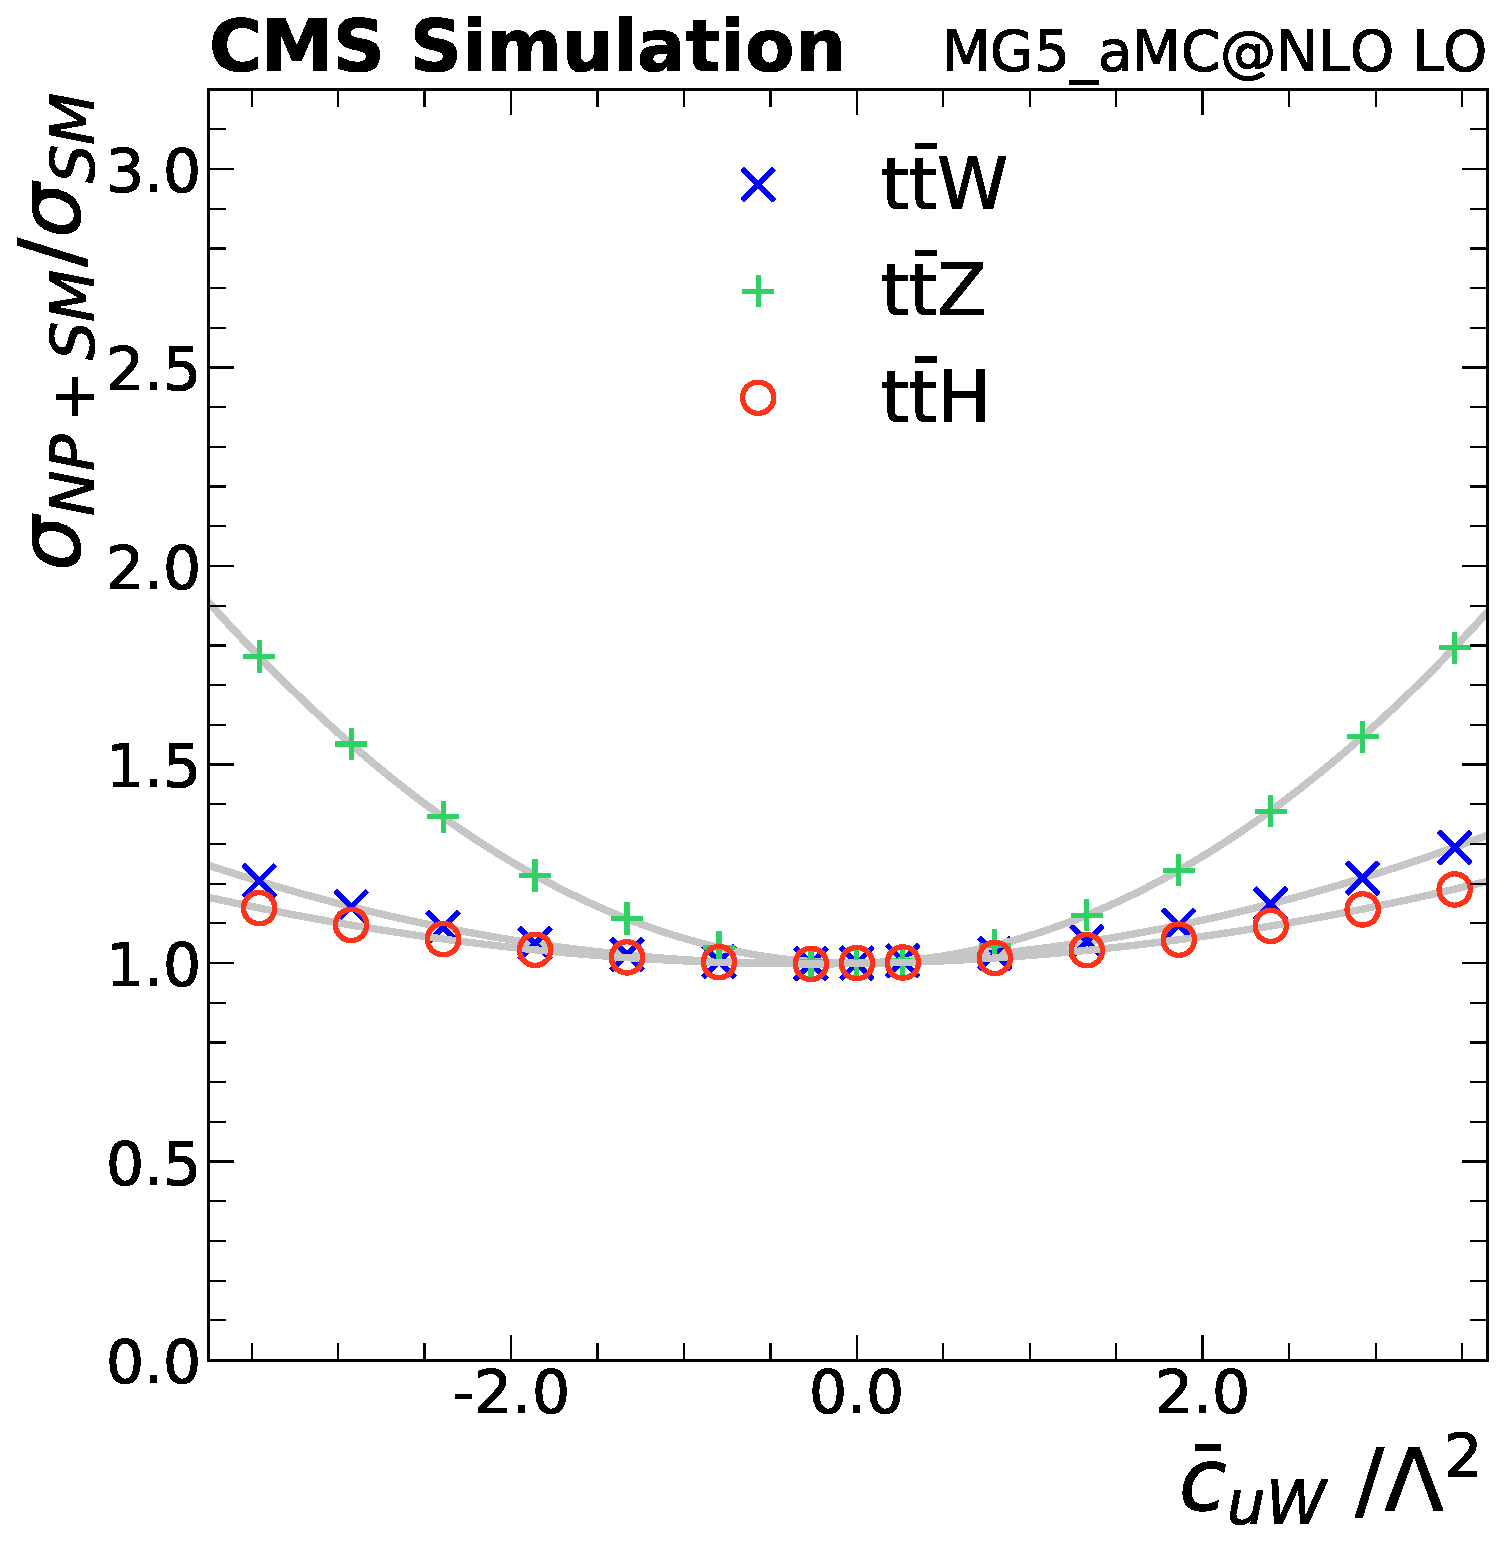
\includegraphics[height=\textheight]{figures/thirteen-TeV/NP/mu/cuW}\hspace{1cm}
        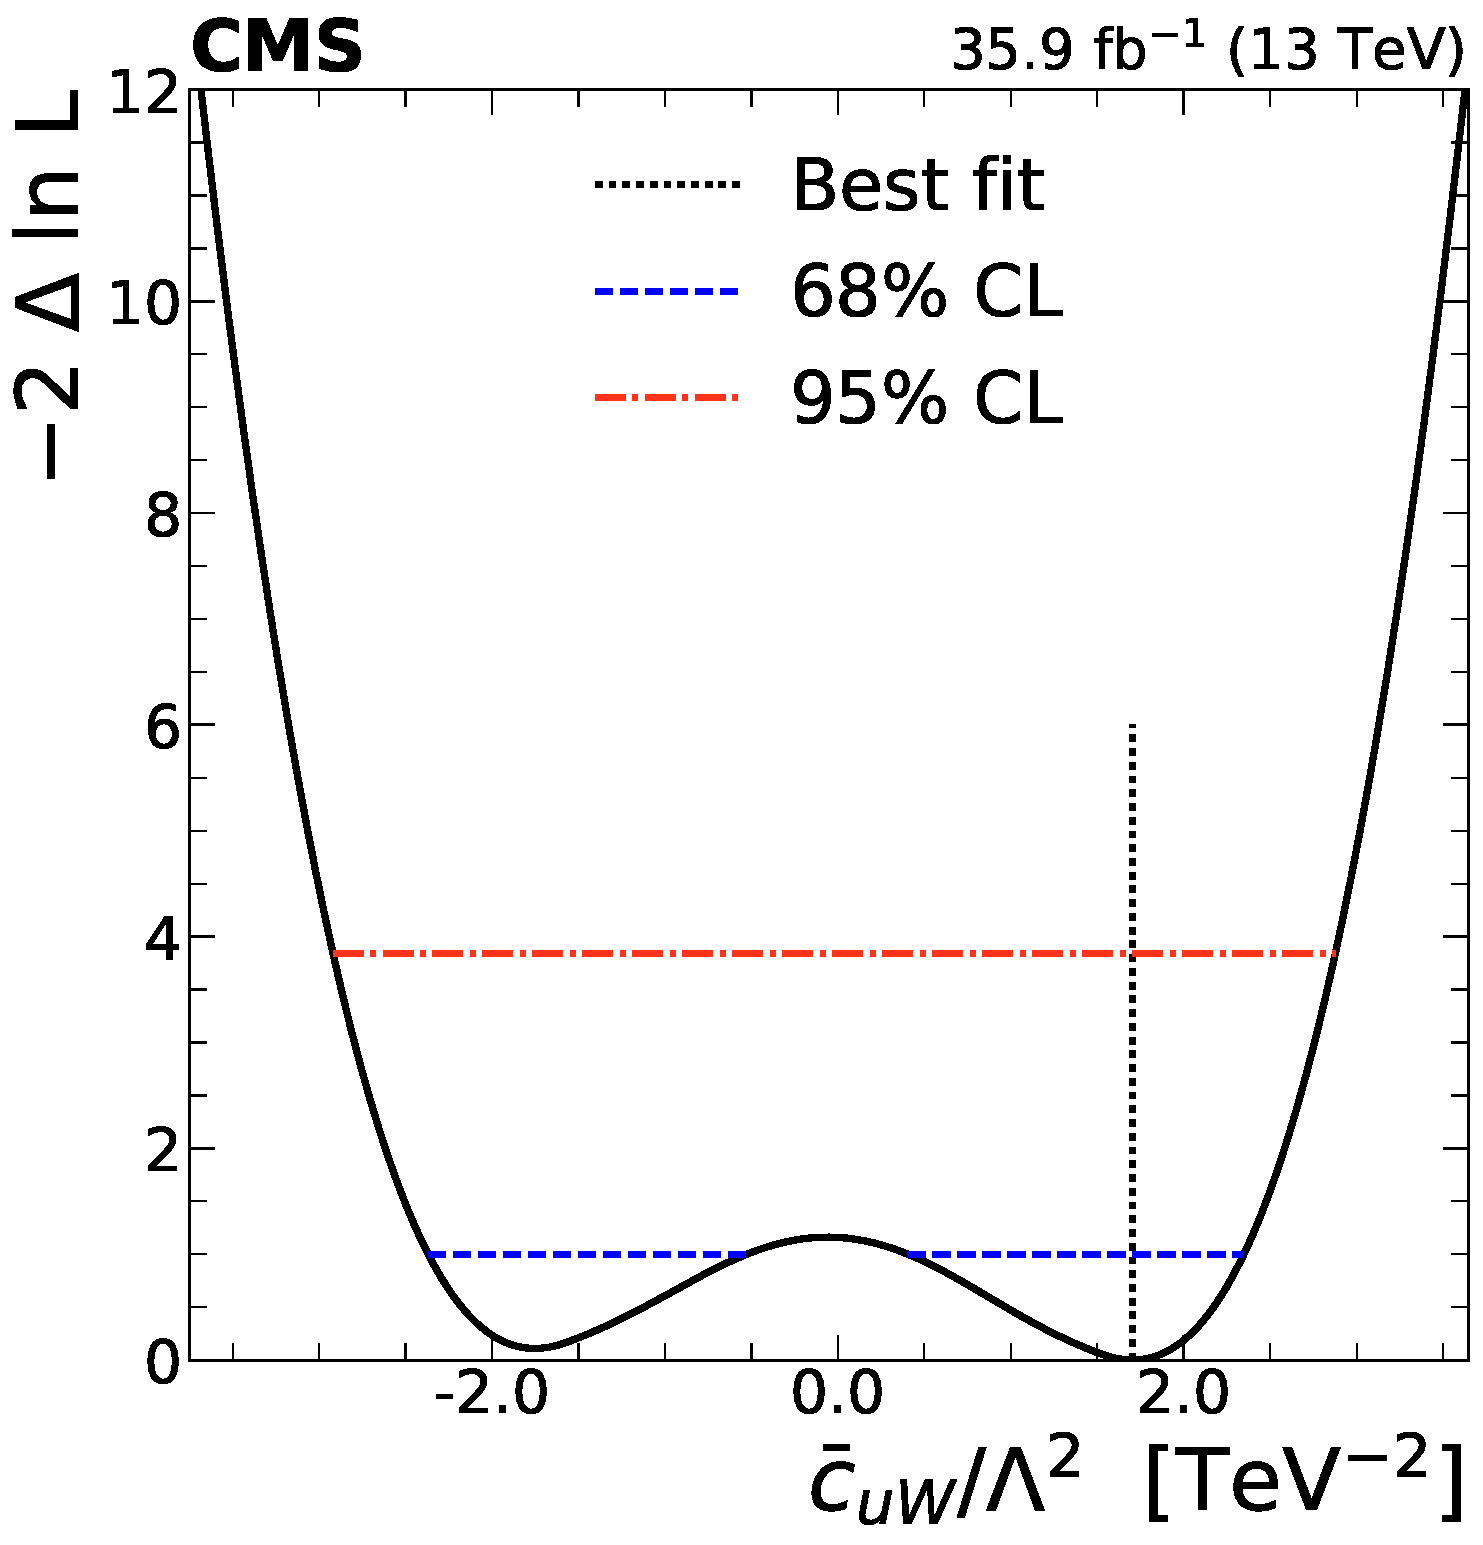
\includegraphics[height=\textheight]{figures/thirteen-TeV/NP/nll/cuW}\hspace{1cm}
        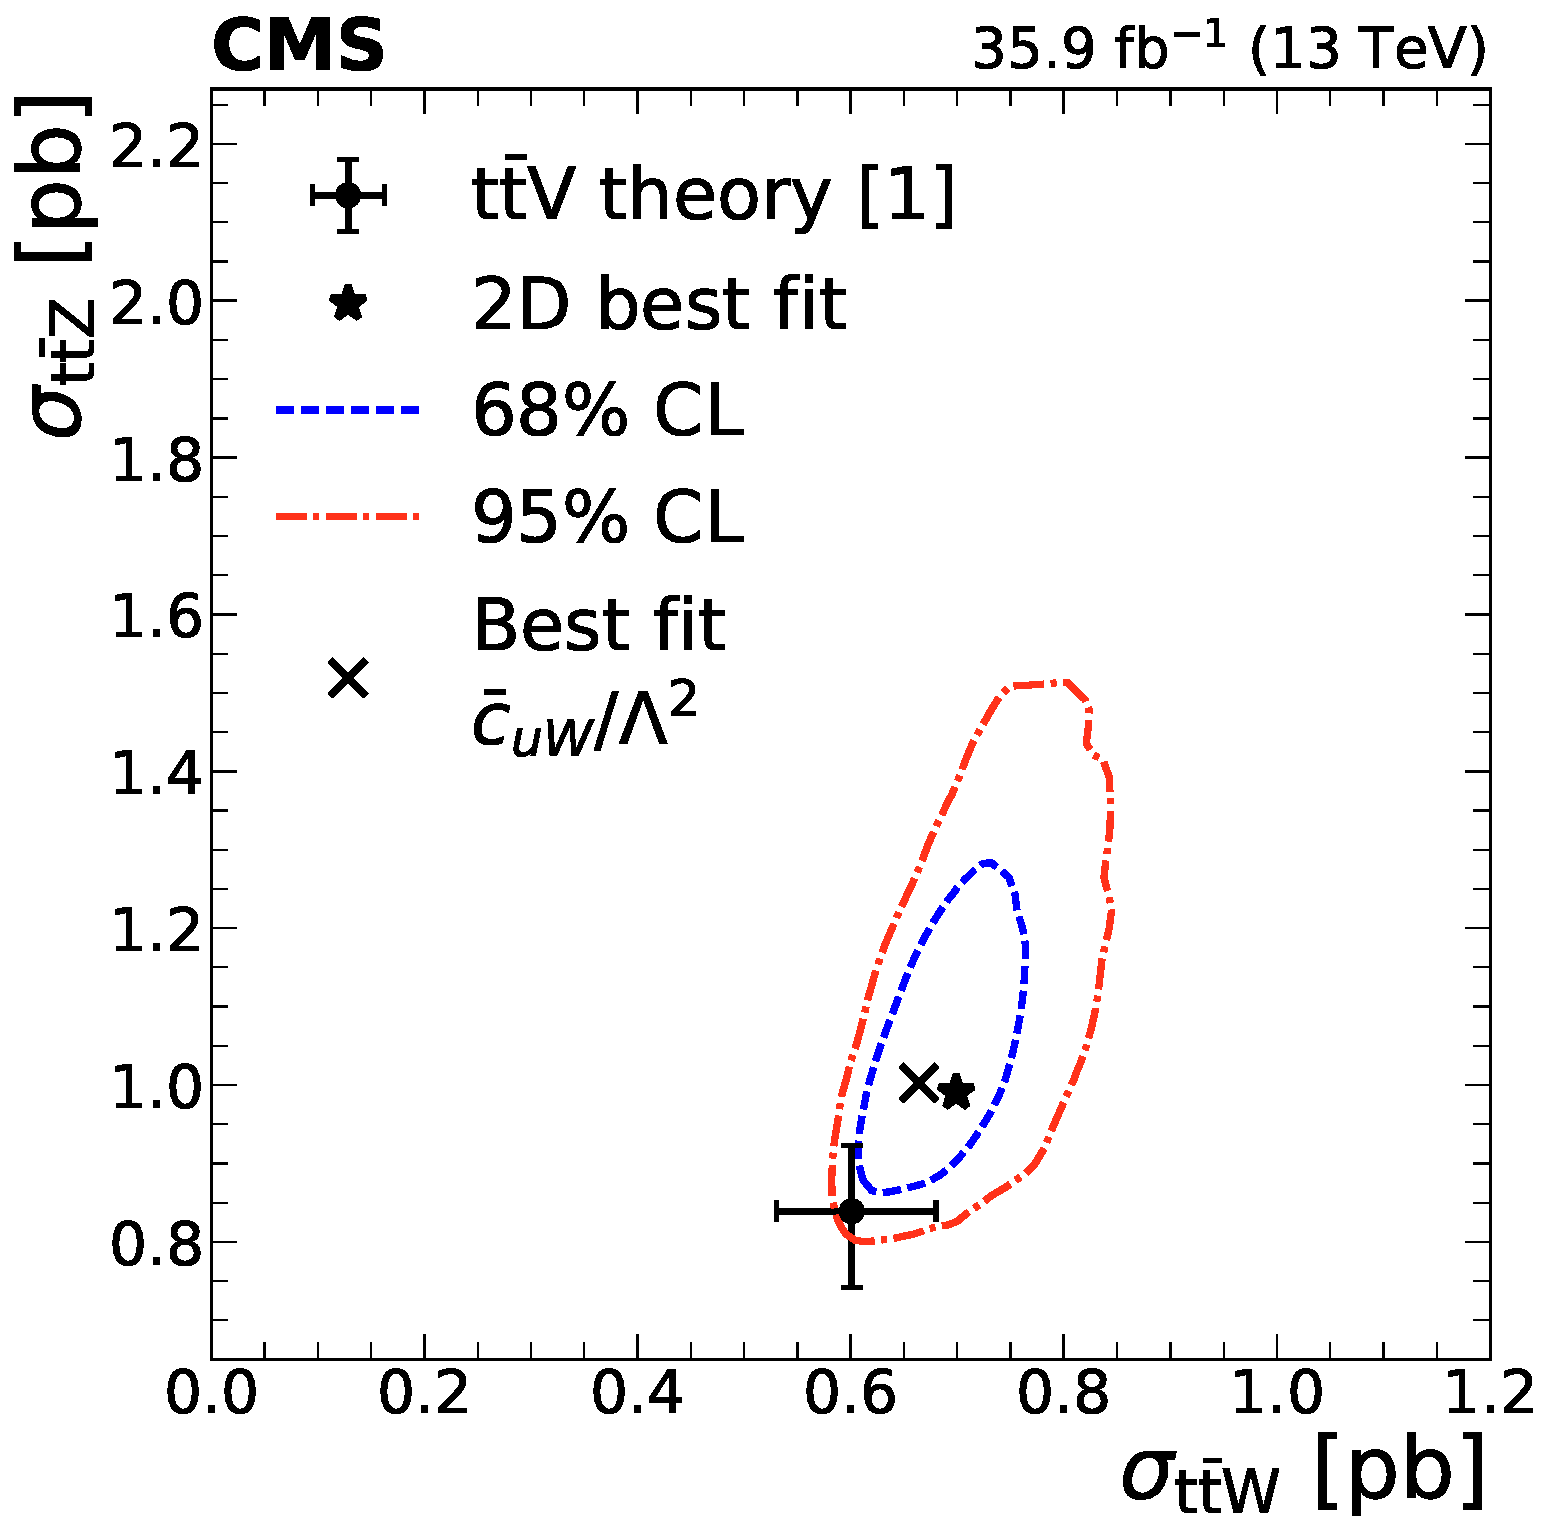
\includegraphics[height=\textheight]{figures/thirteen-TeV/NP/2D/ttZ_ttW_2D_1D_cuW}
      }
    \setlength{\capwidth}{14cm}
    \caption[Profile likelihood, $\mu(c_1)$, and best fit $c_1$ for \cuW (\thirteenTeV)]{Left: signal scaling as a function of the $c_1$ for \ttW (crosses), \ttZ (pluses), and \ttH (circles) for \cuW (\thirteenTeV analysis). Center: the test statistic $q(c_i)$ scan as a function of $c_1$, profiling all other nuisance parameters. The best fit value is indicated by a dotted line. Dashed and dash-dotted lines indicate \SI{68}{\percent} and \SI{95}{\percent} CL intervals, respectively. Right: The best fit $c_1$ value (shown as a cross), along with the corresponding \SI{68}{\percent} (dashed) and \SI{95}{\percent} (dash-dotted) contours in the $\sigma_{\ttZ}, \sigma_{\ttW}$ plane. The two-dimensional best fit to the \ttW and \ttZ cross sections is given by the star. The theory predictions~\cite{deFlorian:2016spz} are shown as a dot with bars representing their respective uncertainties.}%
    \label{fig:results-cuW}
  \end{figure}
  \begin{figure}
      \resizebox{!}{7.2cm}{
        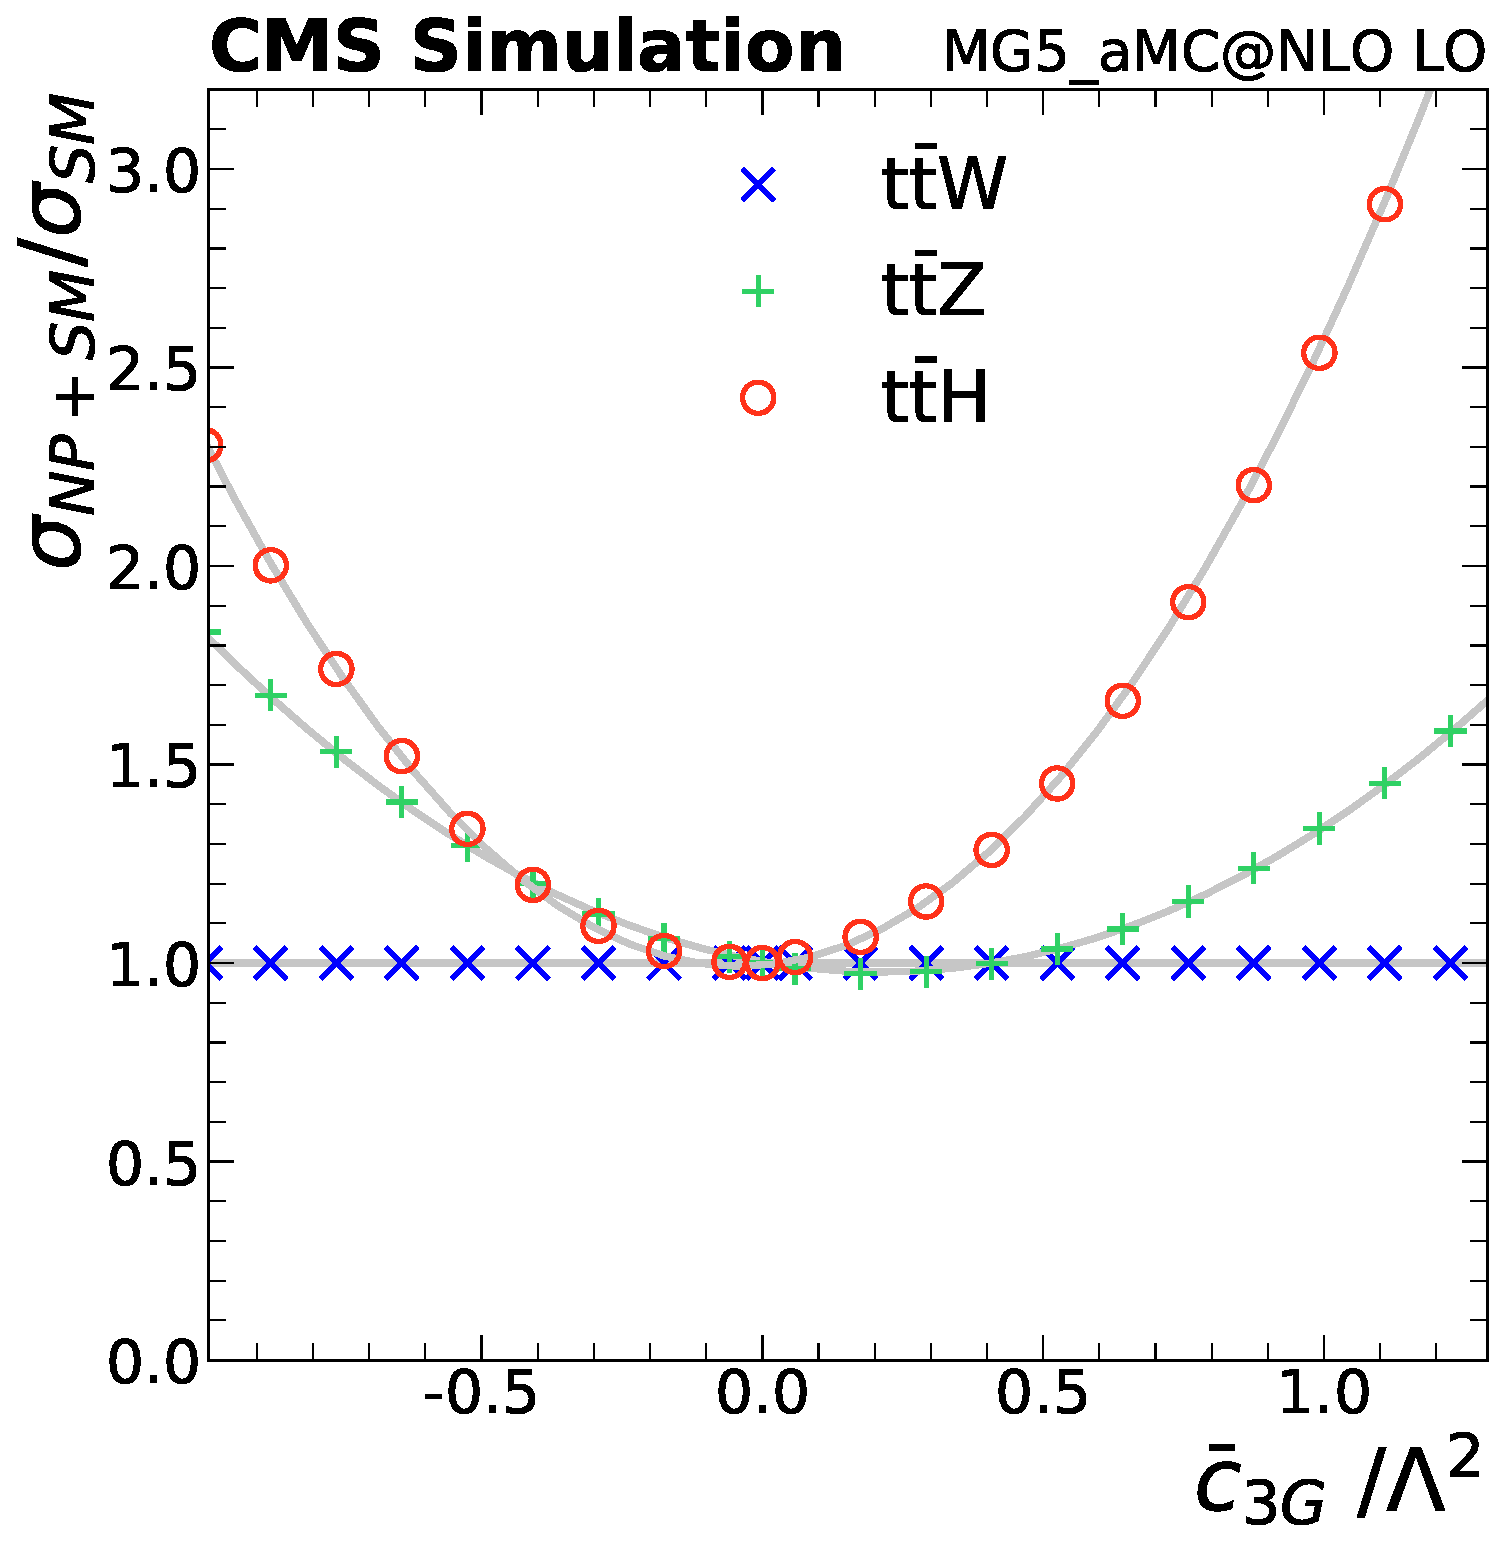
\includegraphics[height=\textheight]{figures/thirteen-TeV/NP/mu/c3G}\hspace{1cm}
        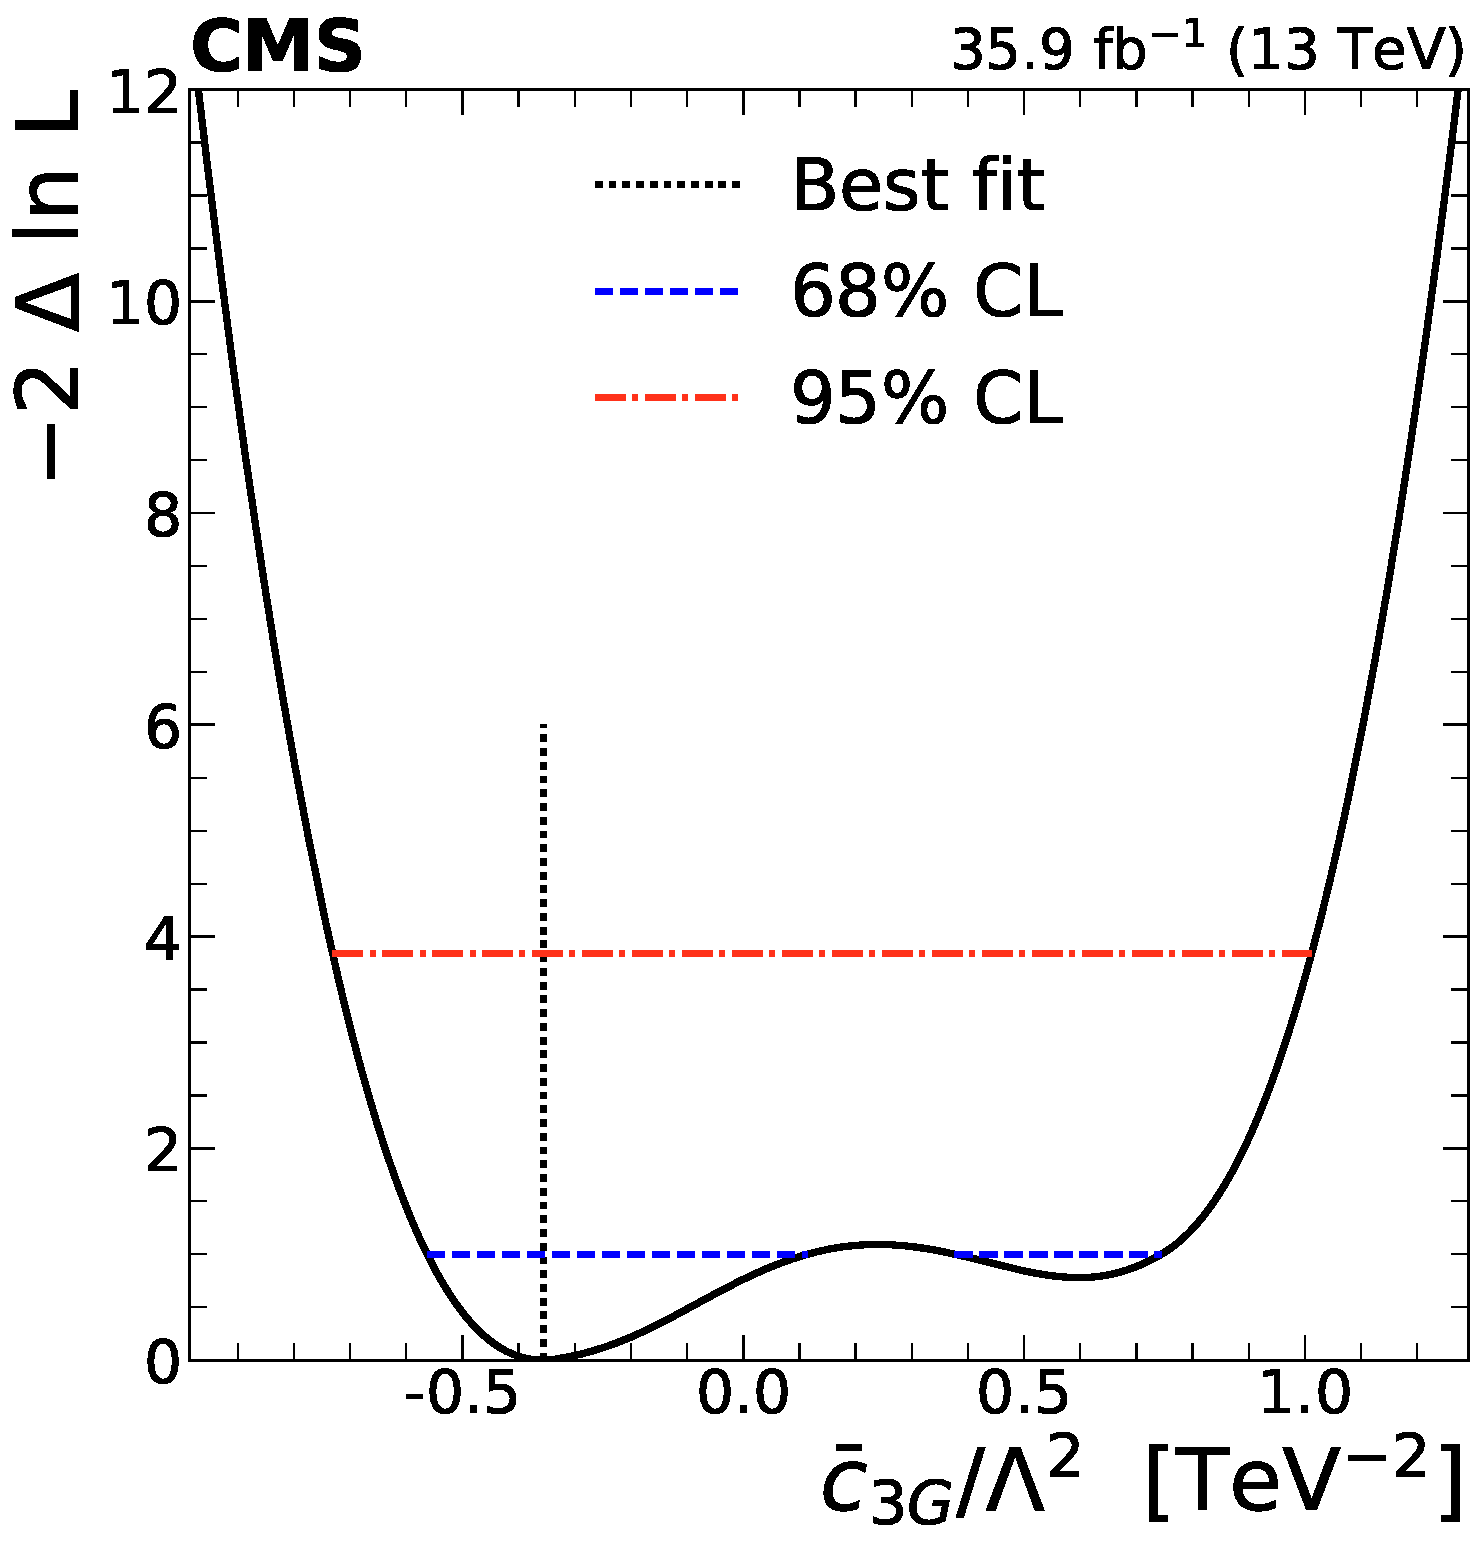
\includegraphics[height=\textheight]{figures/thirteen-TeV/NP/nll/c3G}\hspace{1cm}
        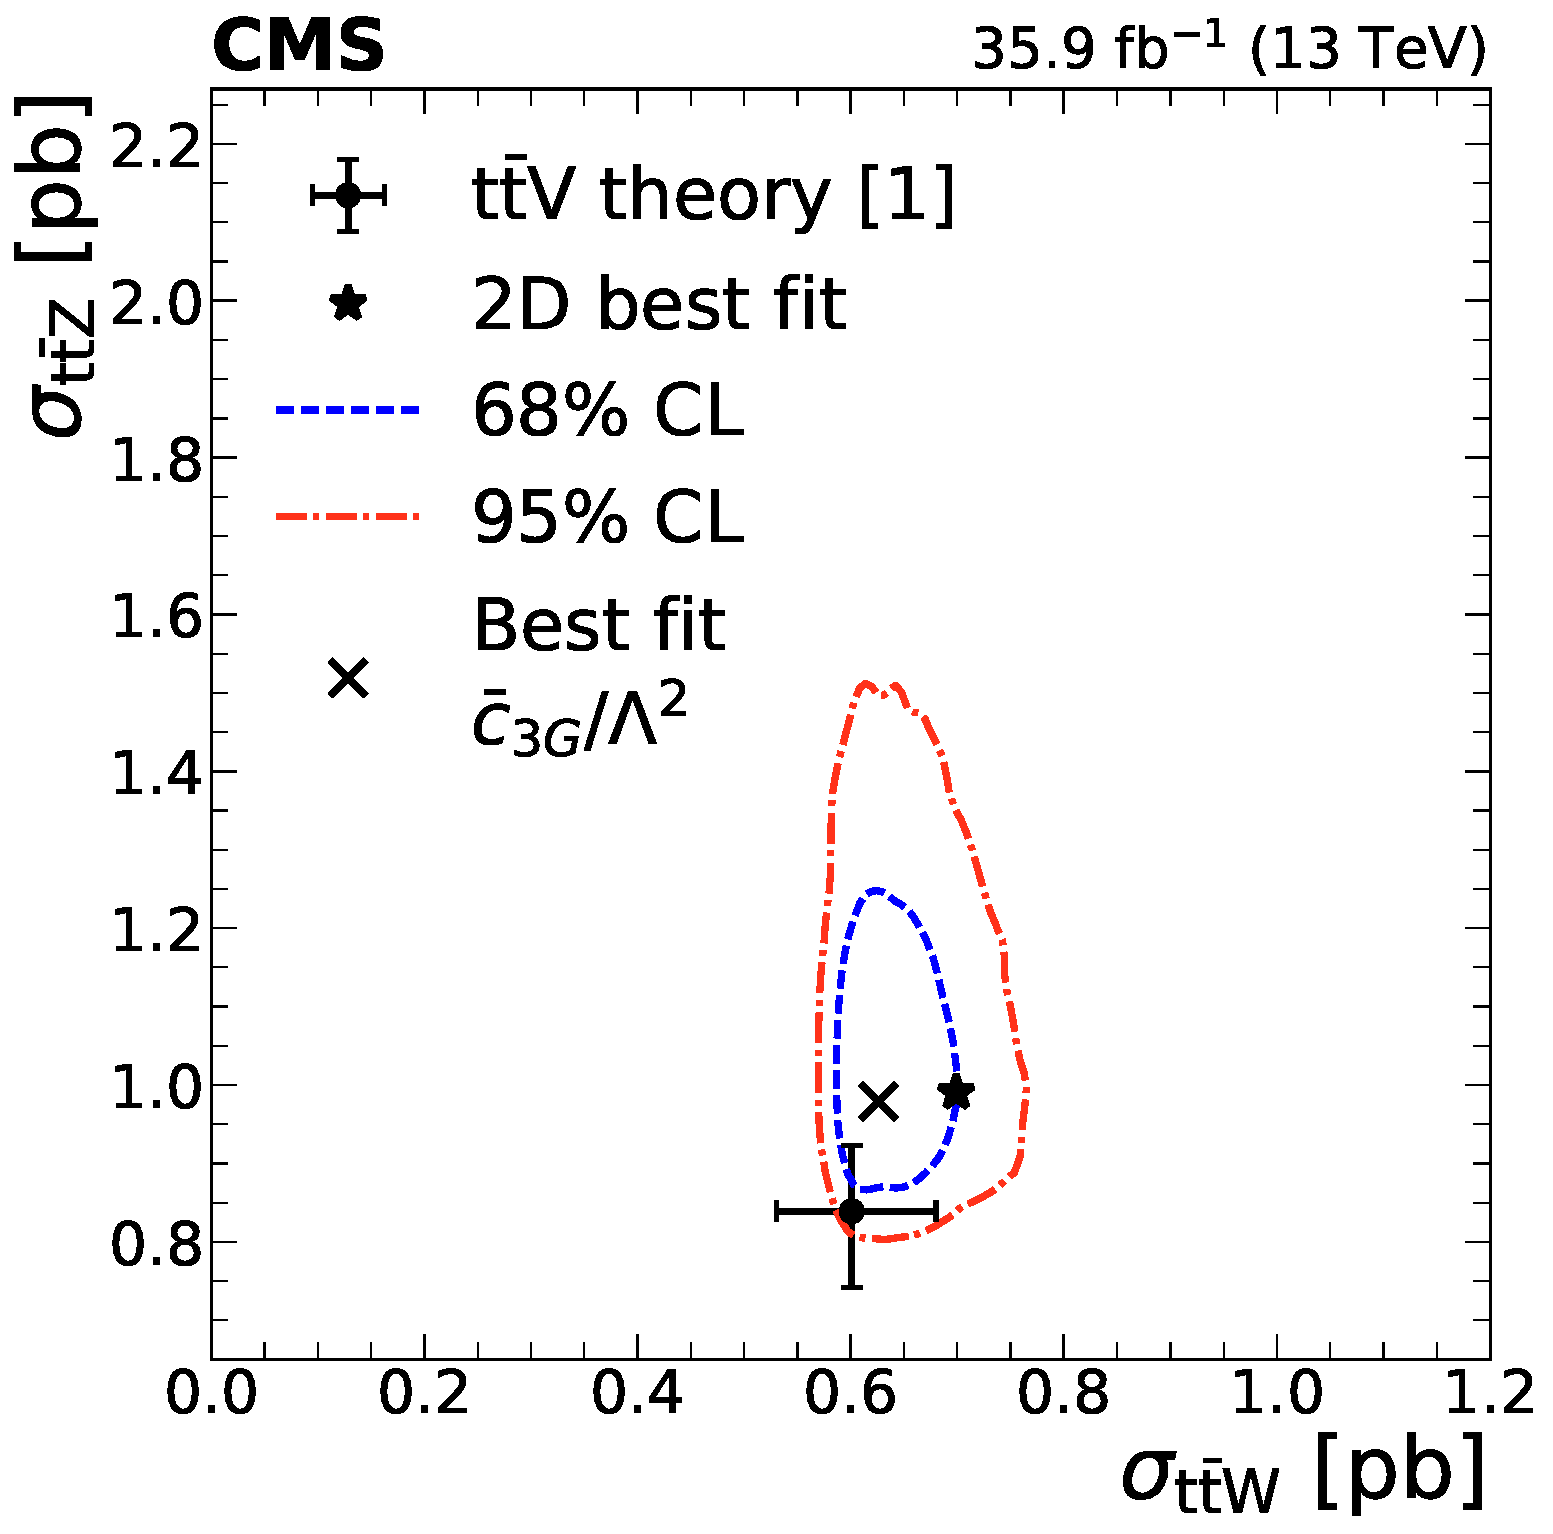
\includegraphics[height=\textheight]{figures/thirteen-TeV/NP/2D/ttZ_ttW_2D_1D_c3G}
      }
    \setlength{\capwidth}{14cm}
    \caption[Profile likelihood, $\mu(c_1)$, and best fit $c_1$ for \cthreeG (\thirteenTeV)]{Left: signal scaling as a function of the $c_1$ for \ttW (crosses), \ttZ (pluses), and \ttH (circles) for \cthreeG (\thirteenTeV analysis). Center: the test statistic $q(c_i)$ scan as a function of $c_1$, profiling all other nuisance parameters. The best fit value is indicated by a dotted line. Dashed and dash-dotted lines indicate \SI{68}{\percent} and \SI{95}{\percent} CL intervals, respectively. Right: The best fit $c_1$ value (shown as a cross), along with the corresponding \SI{68}{\percent} (dashed) and \SI{95}{\percent} (dash-dotted) contours in the $\sigma_{\ttZ}, \sigma_{\ttW}$ plane. The two-dimensional best fit to the \ttW and \ttZ cross sections is given by the star. The theory predictions~\cite{deFlorian:2016spz} are shown as a dot with bars representing their respective uncertainties.}
    \label{fig:results-c3G}
  \end{figure}
  \begin{figure}
      \resizebox{!}{7.2cm}{
        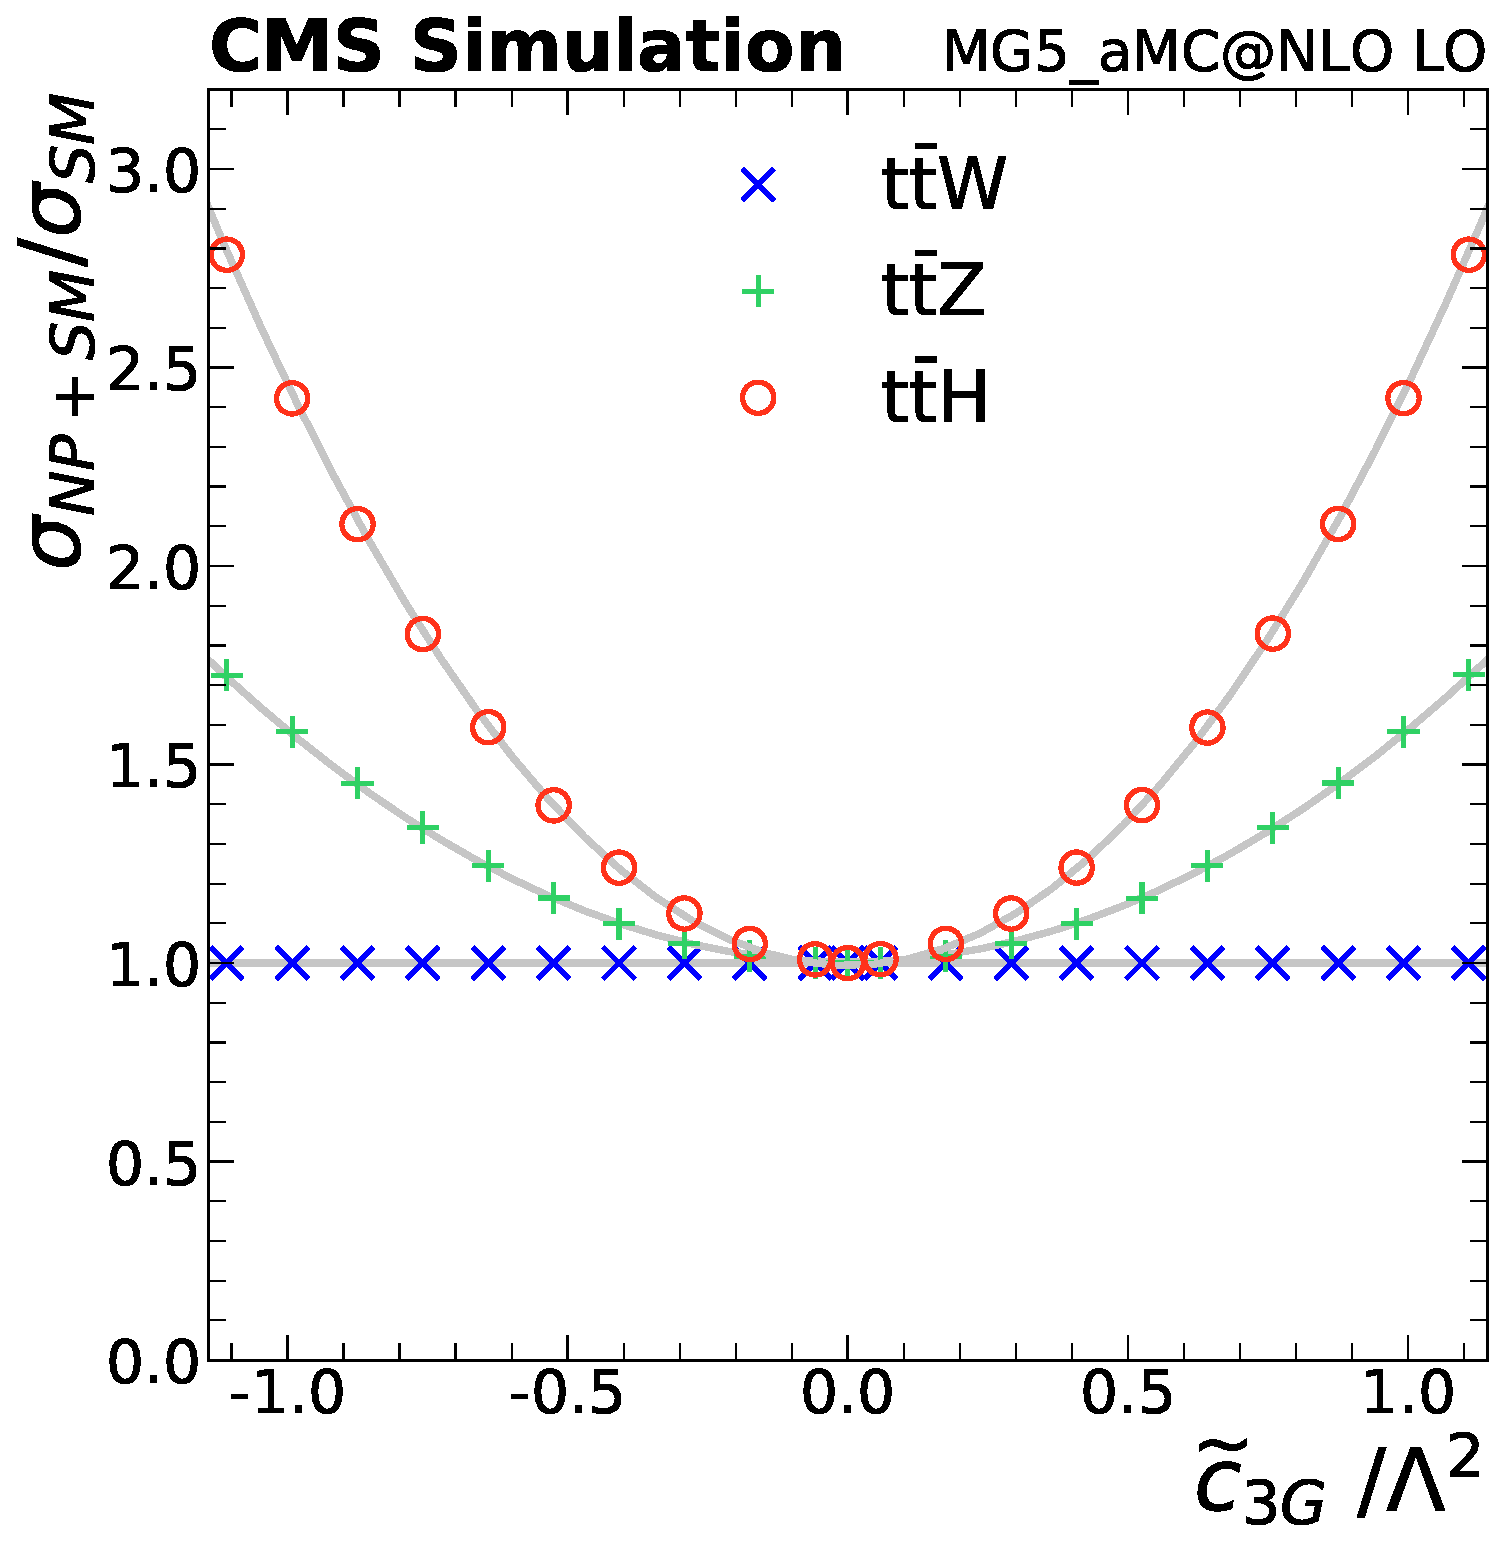
\includegraphics[height=\textheight]{figures/thirteen-TeV/NP/mu/tc3G}\hspace{1cm}
        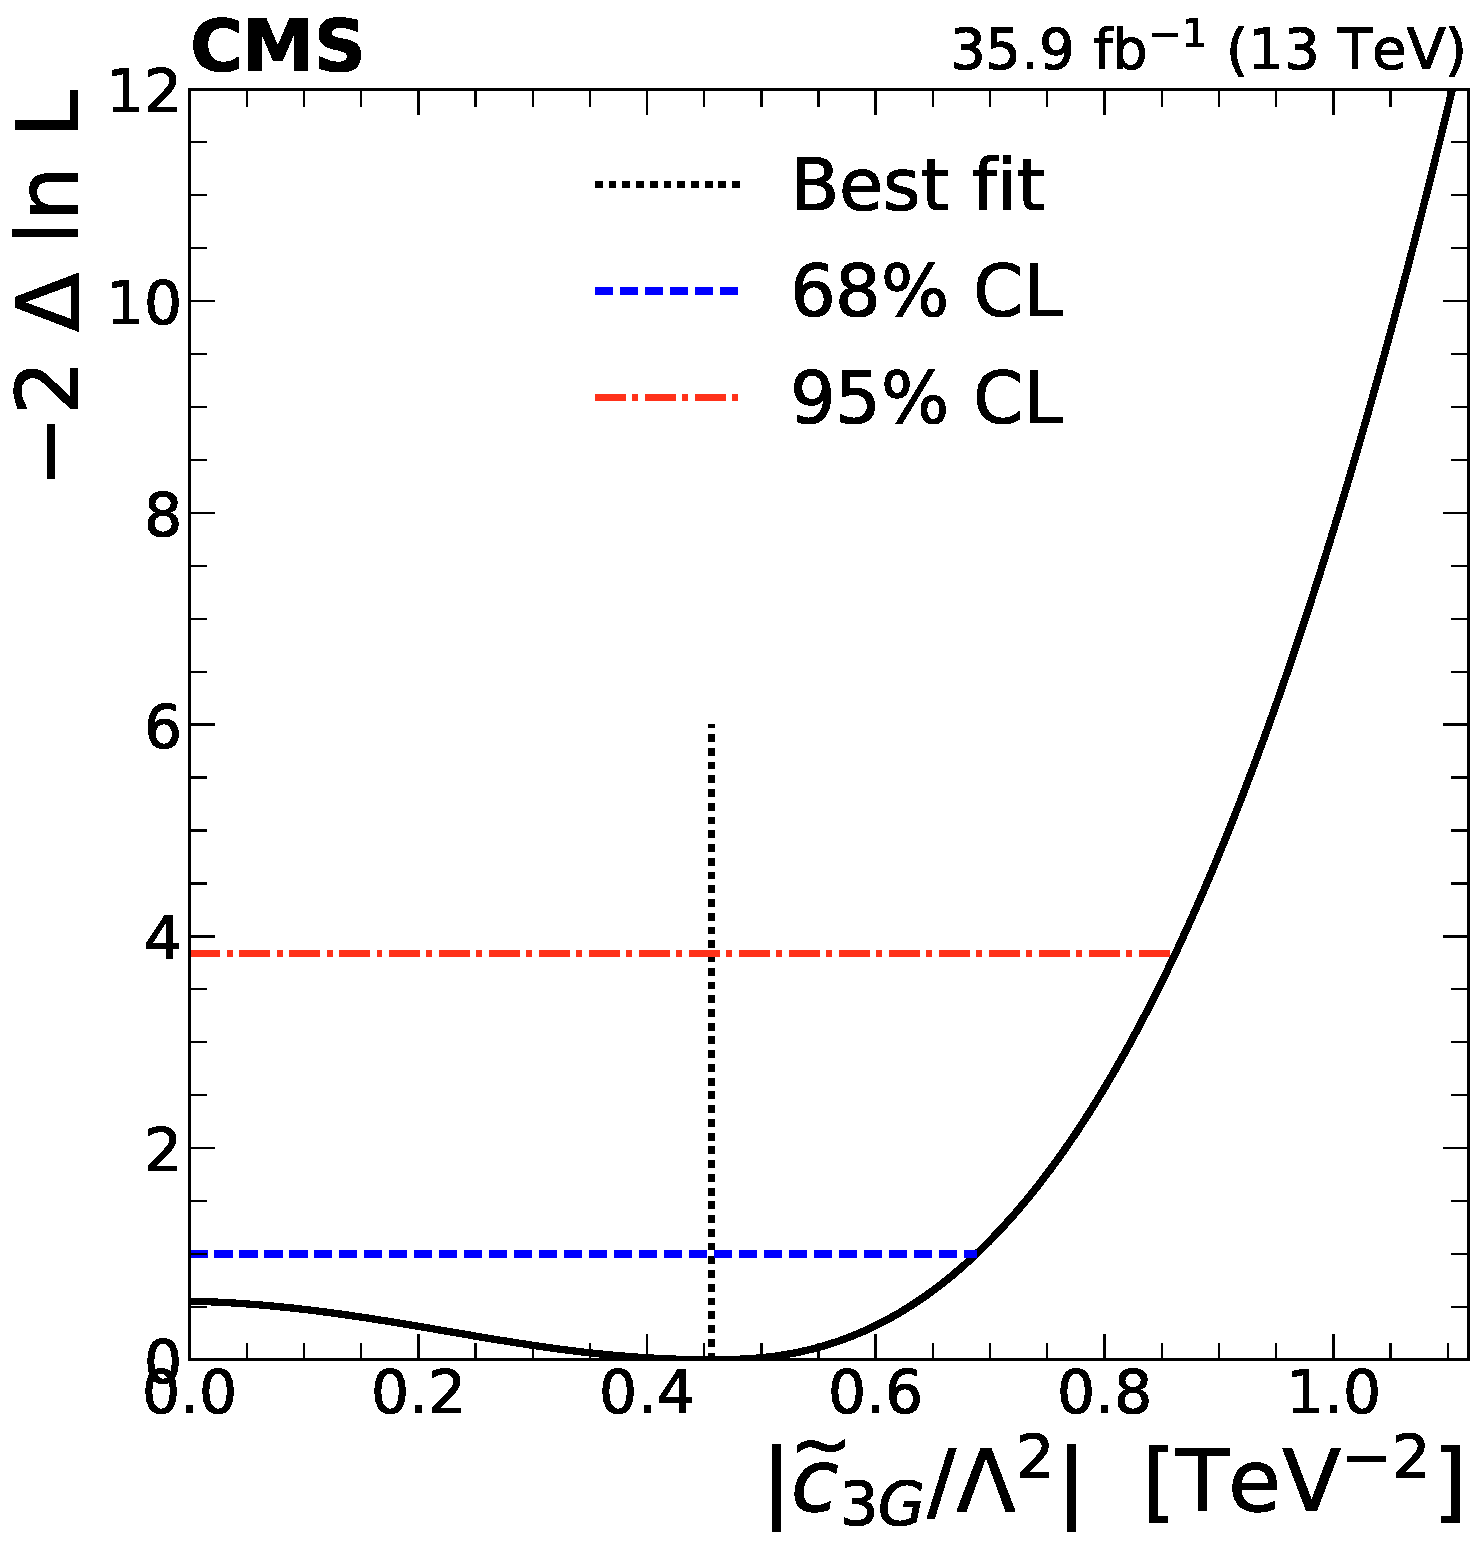
\includegraphics[height=\textheight]{figures/thirteen-TeV/NP/nll/tc3G}\hspace{1cm}
        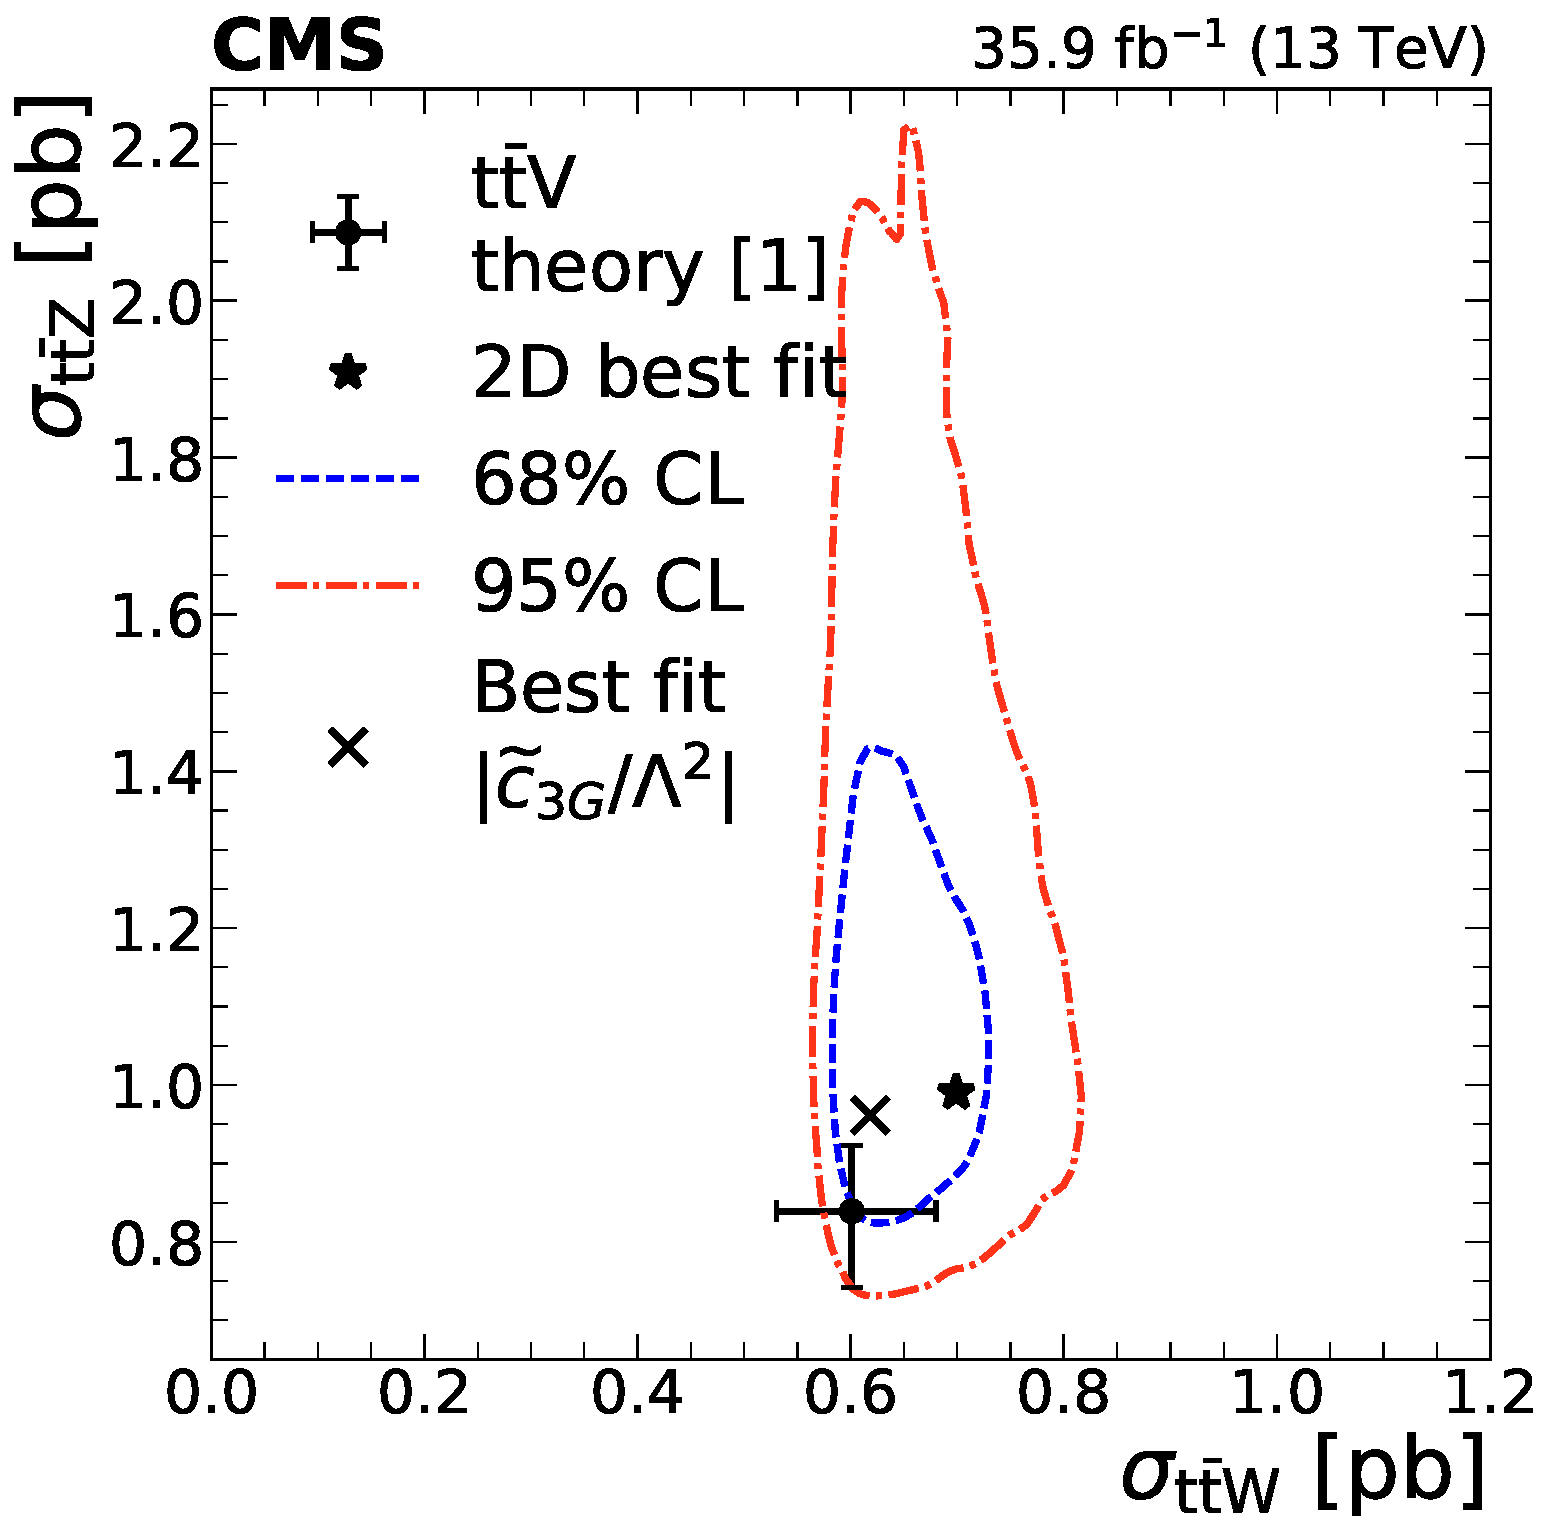
\includegraphics[height=\textheight]{figures/thirteen-TeV/NP/2D/ttZ_ttW_2D_1D_tc3G}
      }
    \setlength{\capwidth}{14cm}
    \caption[Profile likelihood, $\mu(c_1)$, and best fit $c_1$ for \tcthreeG (\thirteenTeV)]{Left: signal scaling as a function of the $c_1$ for \ttW (crosses), \ttZ (pluses), and \ttH (circles) for \tcthreeG (\thirteenTeV analysis). Center: the test statistic $q(c_i)$ scan as a function of $c_1$, profiling all other nuisance parameters. The best fit value is indicated by a dotted line. Dashed and dash-dotted lines indicate \SI{68}{\percent} and \SI{95}{\percent} CL intervals, respectively. Right: The best fit $c_1$ value (shown as a cross), along with the corresponding \SI{68}{\percent} (dashed) and \SI{95}{\percent} (dash-dotted) contours in the $\sigma_{\ttZ}, \sigma_{\ttW}$ plane. The two-dimensional best fit to the \ttW and \ttZ cross sections is given by the star. The theory predictions~\cite{deFlorian:2016spz} are shown as a dot with bars representing their respective uncertainties.}
    \label{fig:results-tc3G}
  \end{figure}
  \begin{figure}
      \resizebox{!}{7.2cm}{
        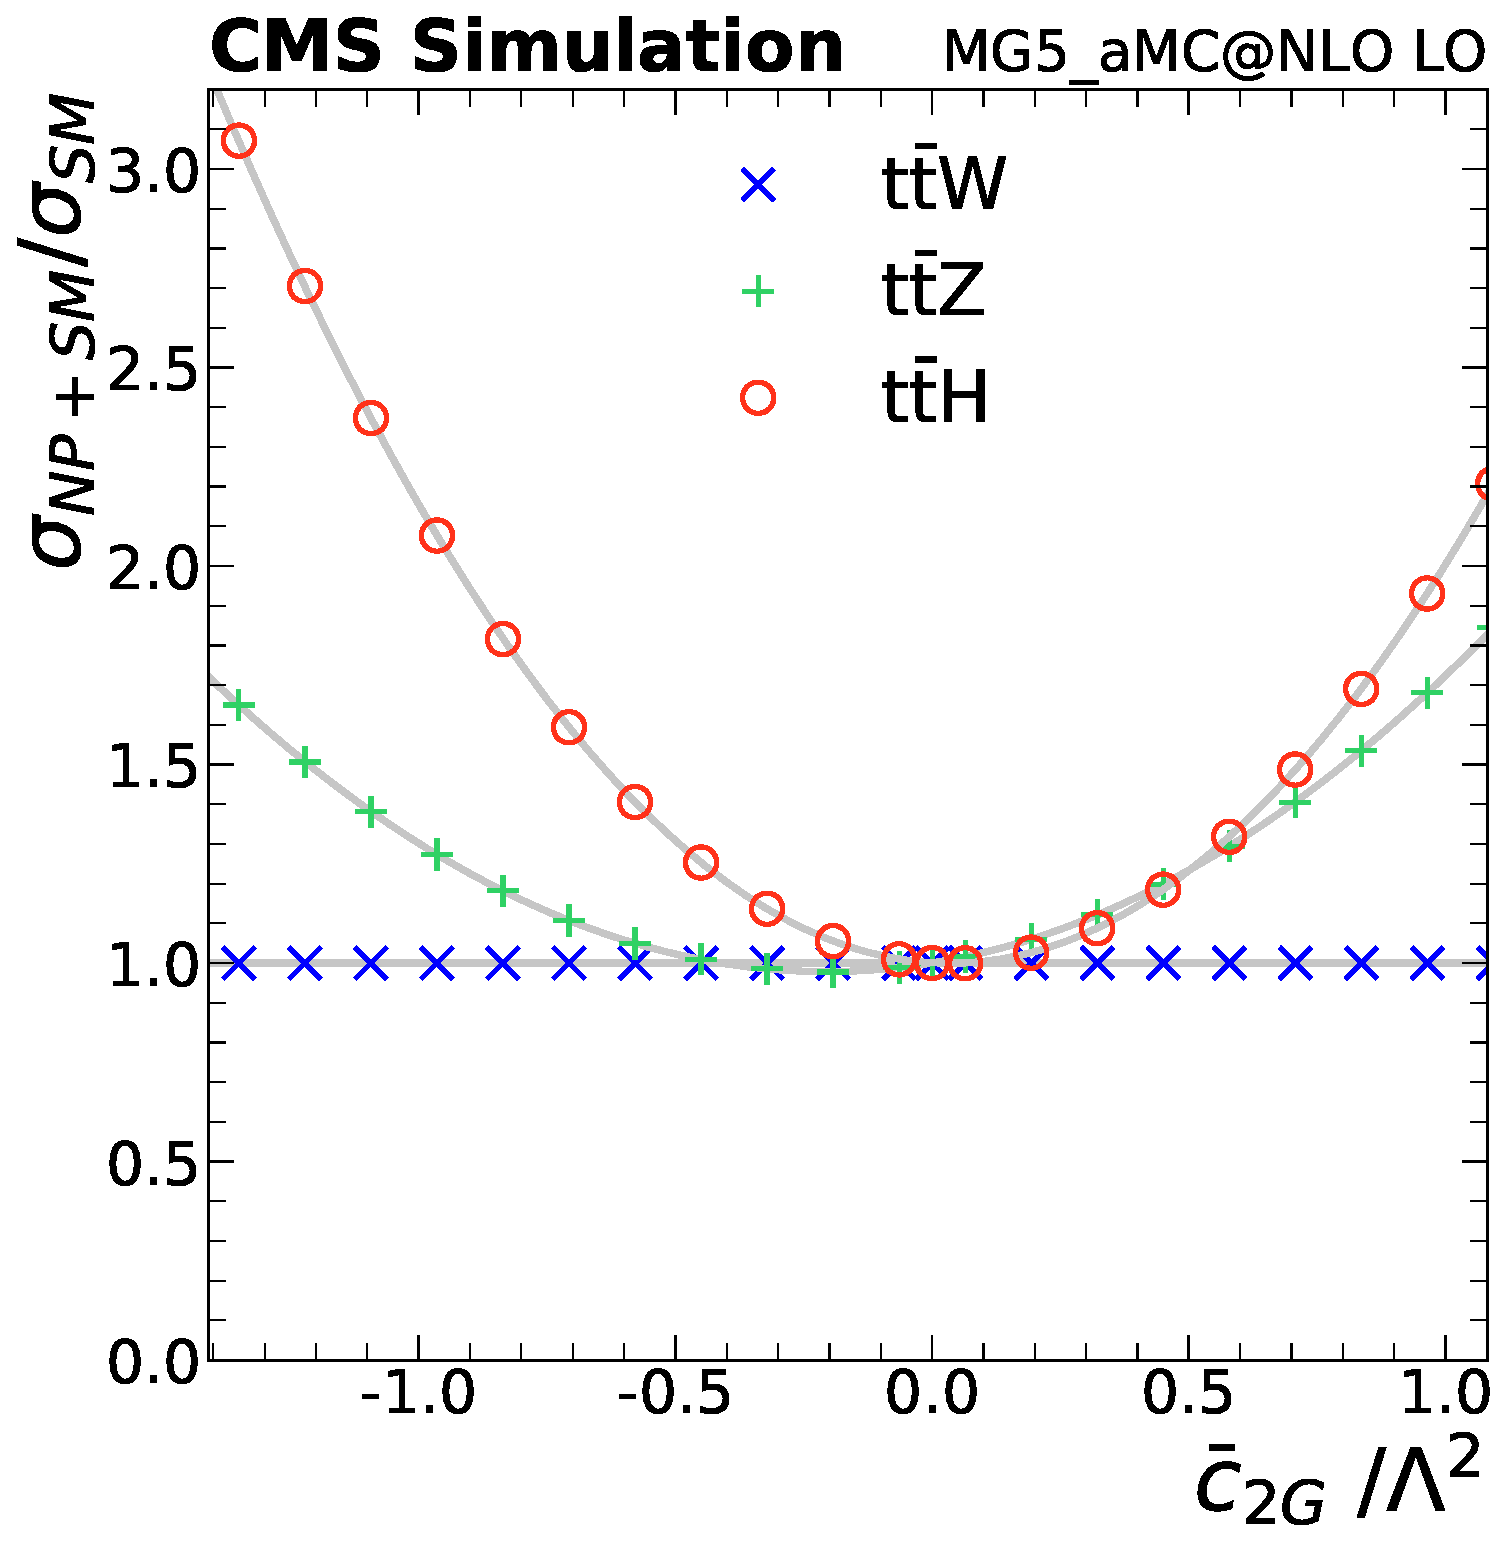
\includegraphics[height=\textheight]{figures/thirteen-TeV/NP/mu/c2G}\hspace{1cm}
        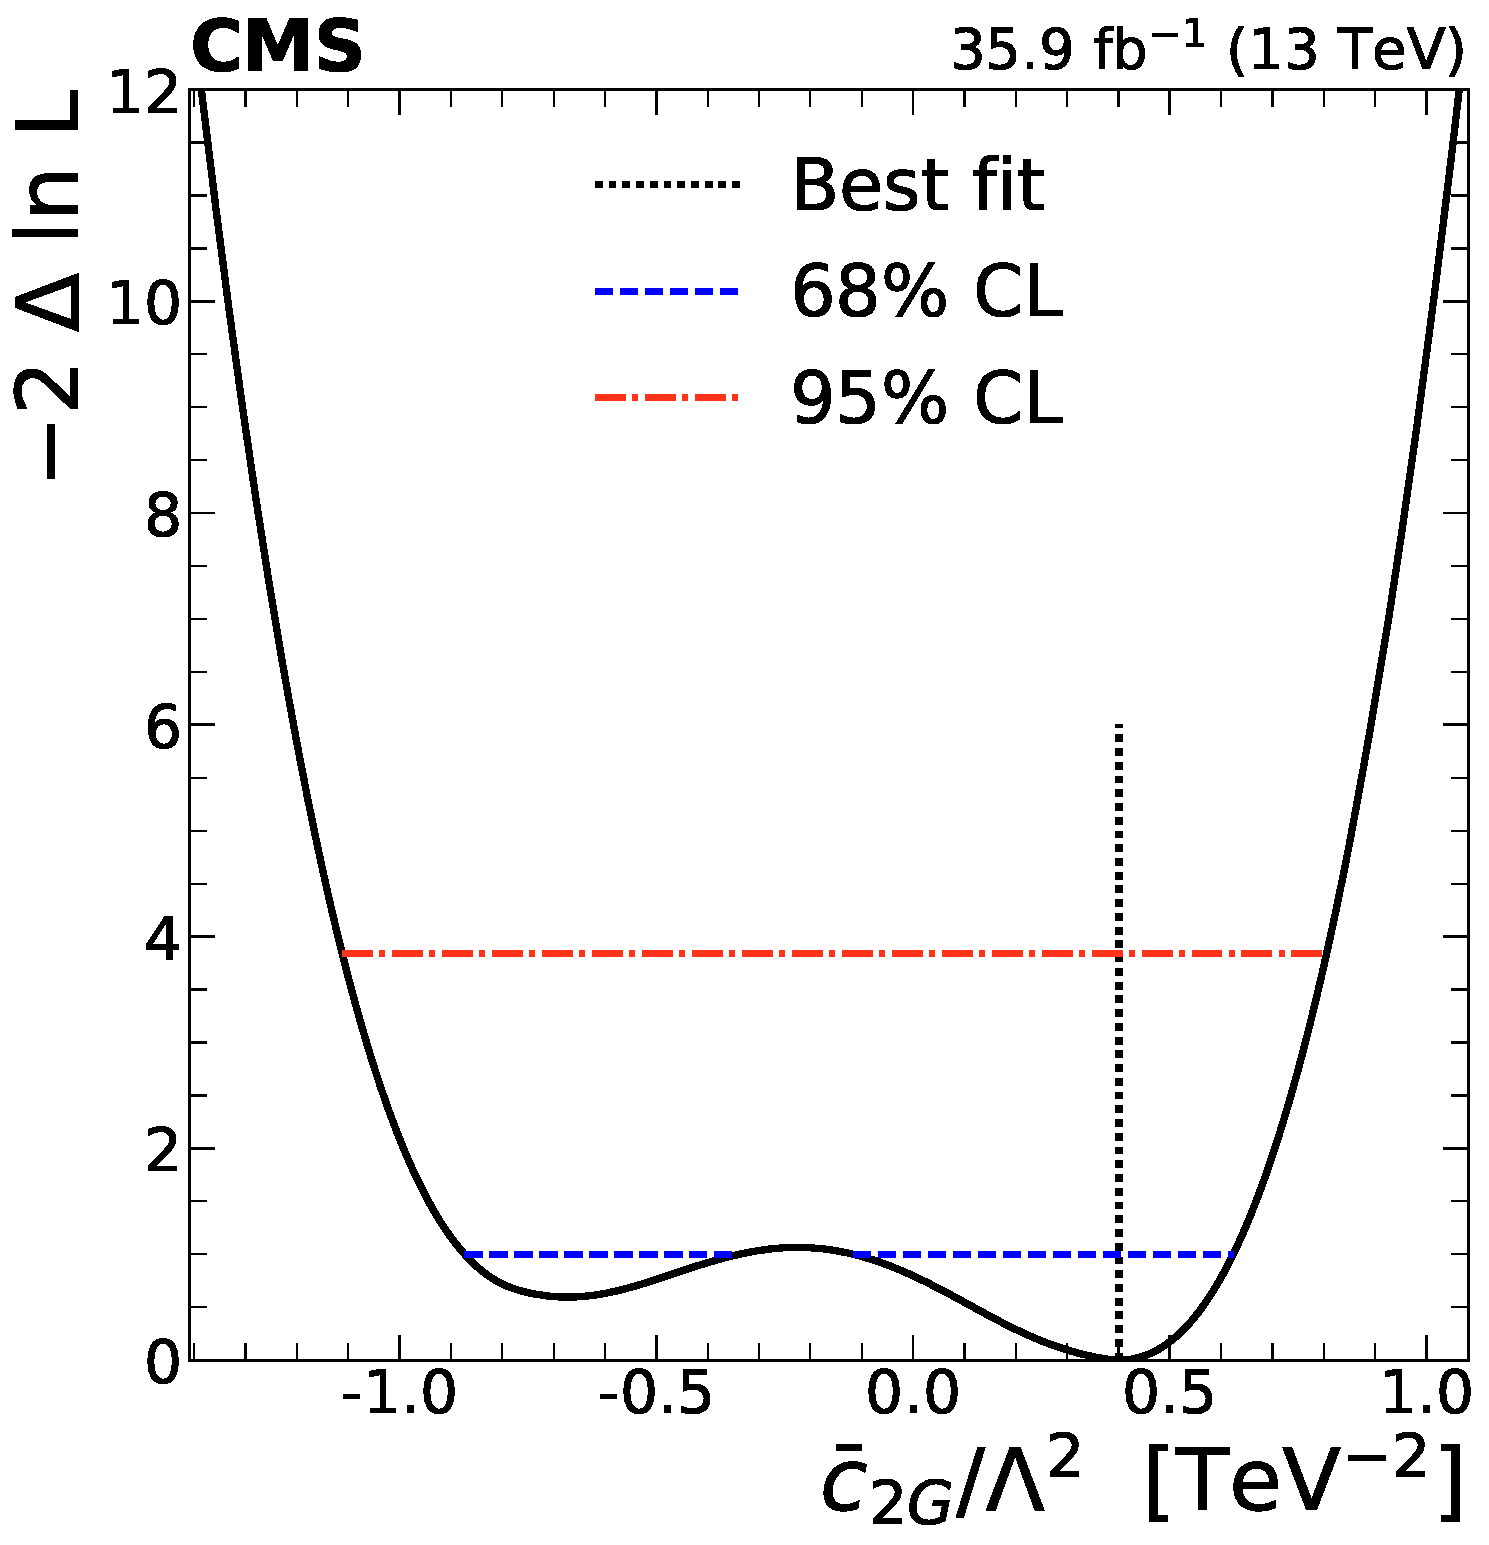
\includegraphics[height=\textheight]{figures/thirteen-TeV/NP/nll/c2G}\hspace{1cm}
        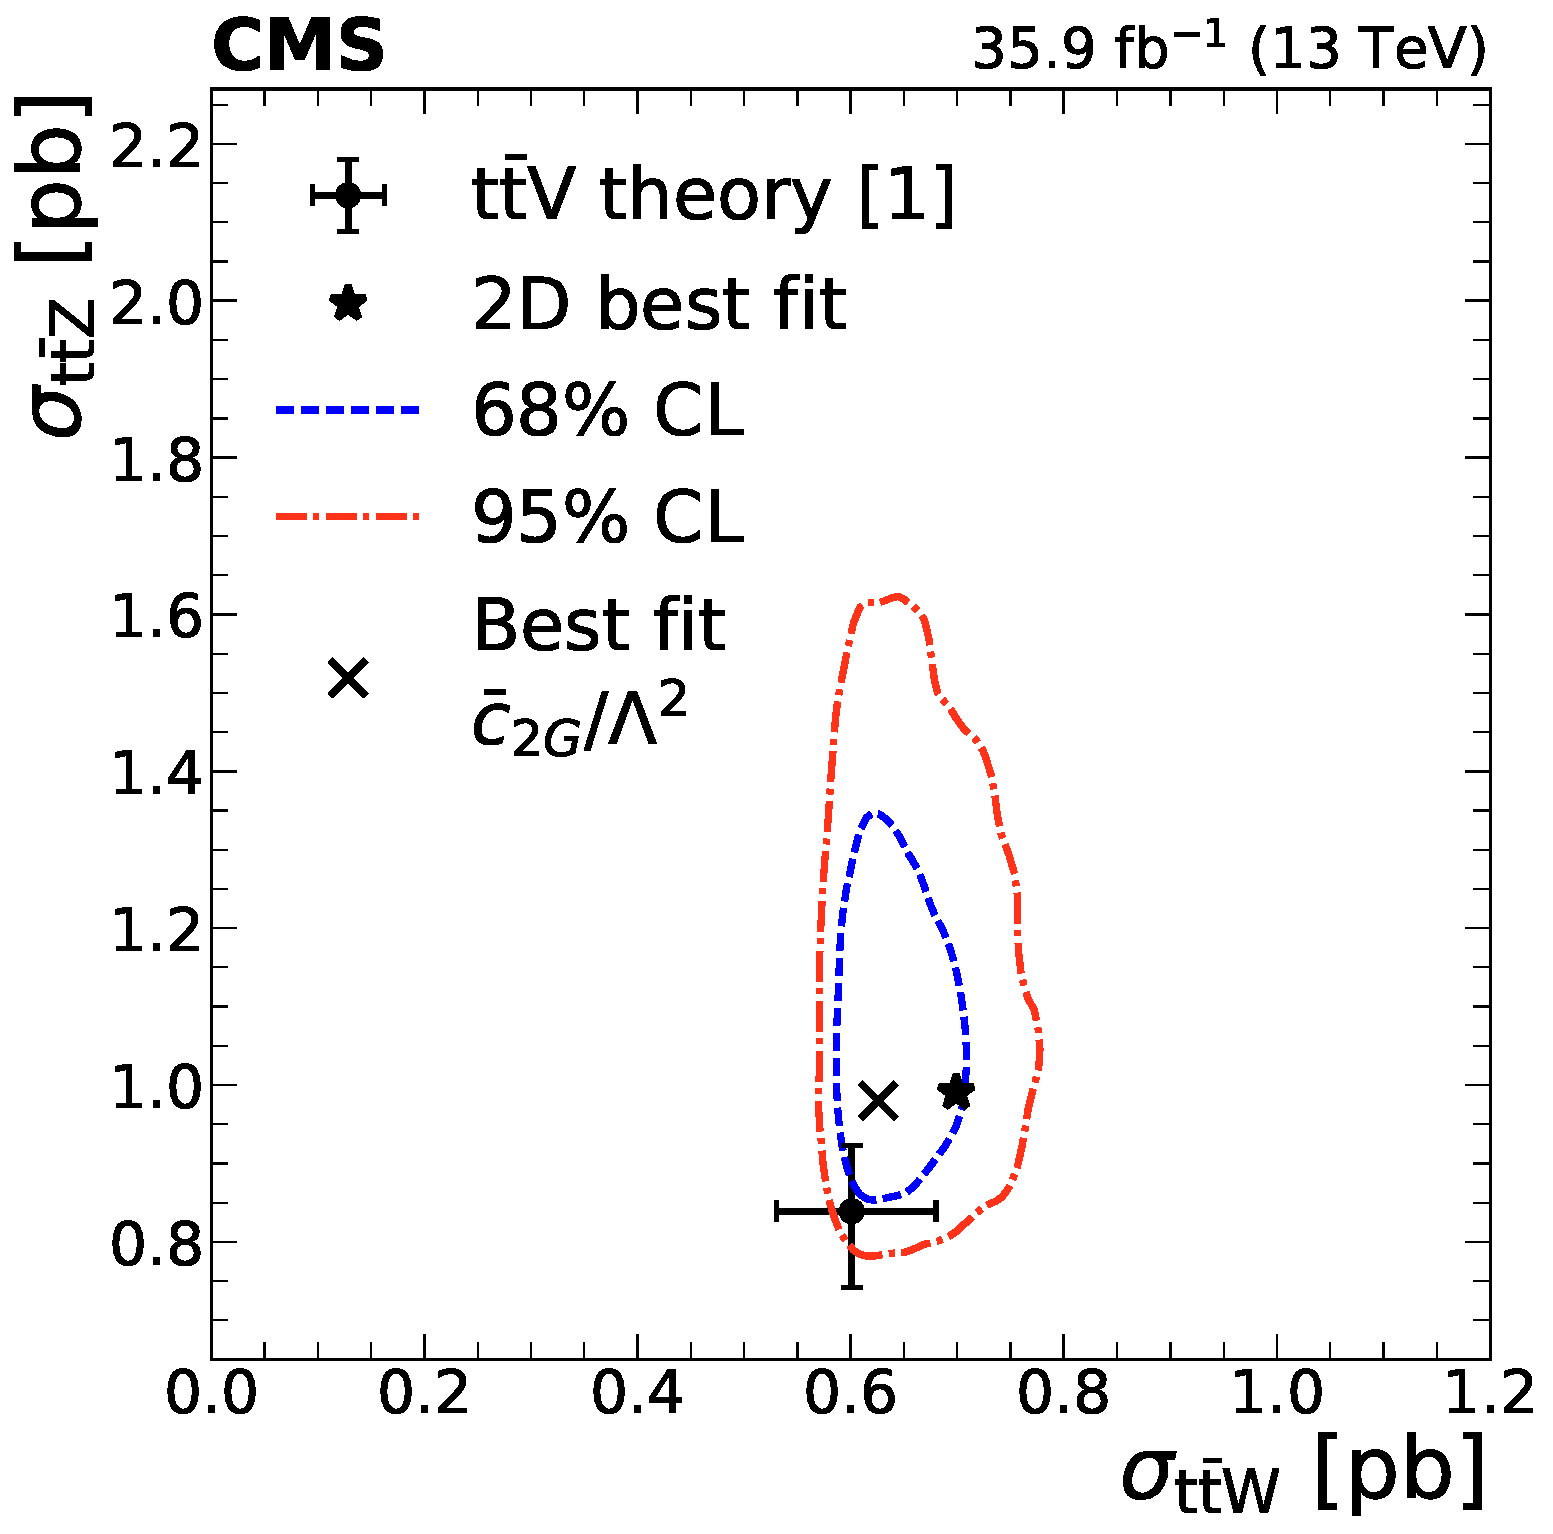
\includegraphics[height=\textheight]{figures/thirteen-TeV/NP/2D/ttZ_ttW_2D_1D_c2G}
      }
    \setlength{\capwidth}{14cm}
    \caption[Profile likelihood, $\mu(c_1)$, and best fit $c_1$ for \ctwoG (\thirteenTeV)]{Left: signal scaling as a function of the $c_1$ for \ttW (crosses), \ttZ (pluses), and \ttH (circles) for \ctwoG (\thirteenTeV analysis). Center: the test statistic $q(c_i)$ scan as a function of $c_1$, profiling all other nuisance parameters. The best fit value is indicated by a dotted line. Dashed and dash-dotted lines indicate \SI{68}{\percent} and \SI{95}{\percent} CL intervals, respectively. Right: The best fit $c_1$ value (shown as a cross), along with the corresponding \SI{68}{\percent} (dashed) and \SI{95}{\percent} (dash-dotted) contours in the $\sigma_{\ttZ}, \sigma_{\ttW}$ plane. The two-dimensional best fit to the \ttW and \ttZ cross sections is given by the star. The theory predictions~\cite{deFlorian:2016spz} are shown as a dot with bars representing their respective uncertainties.}
    \label{fig:results-c2G}
  \end{figure}
  \begin{figure}
      \centering
      \resizebox{!}{7.2cm}{
        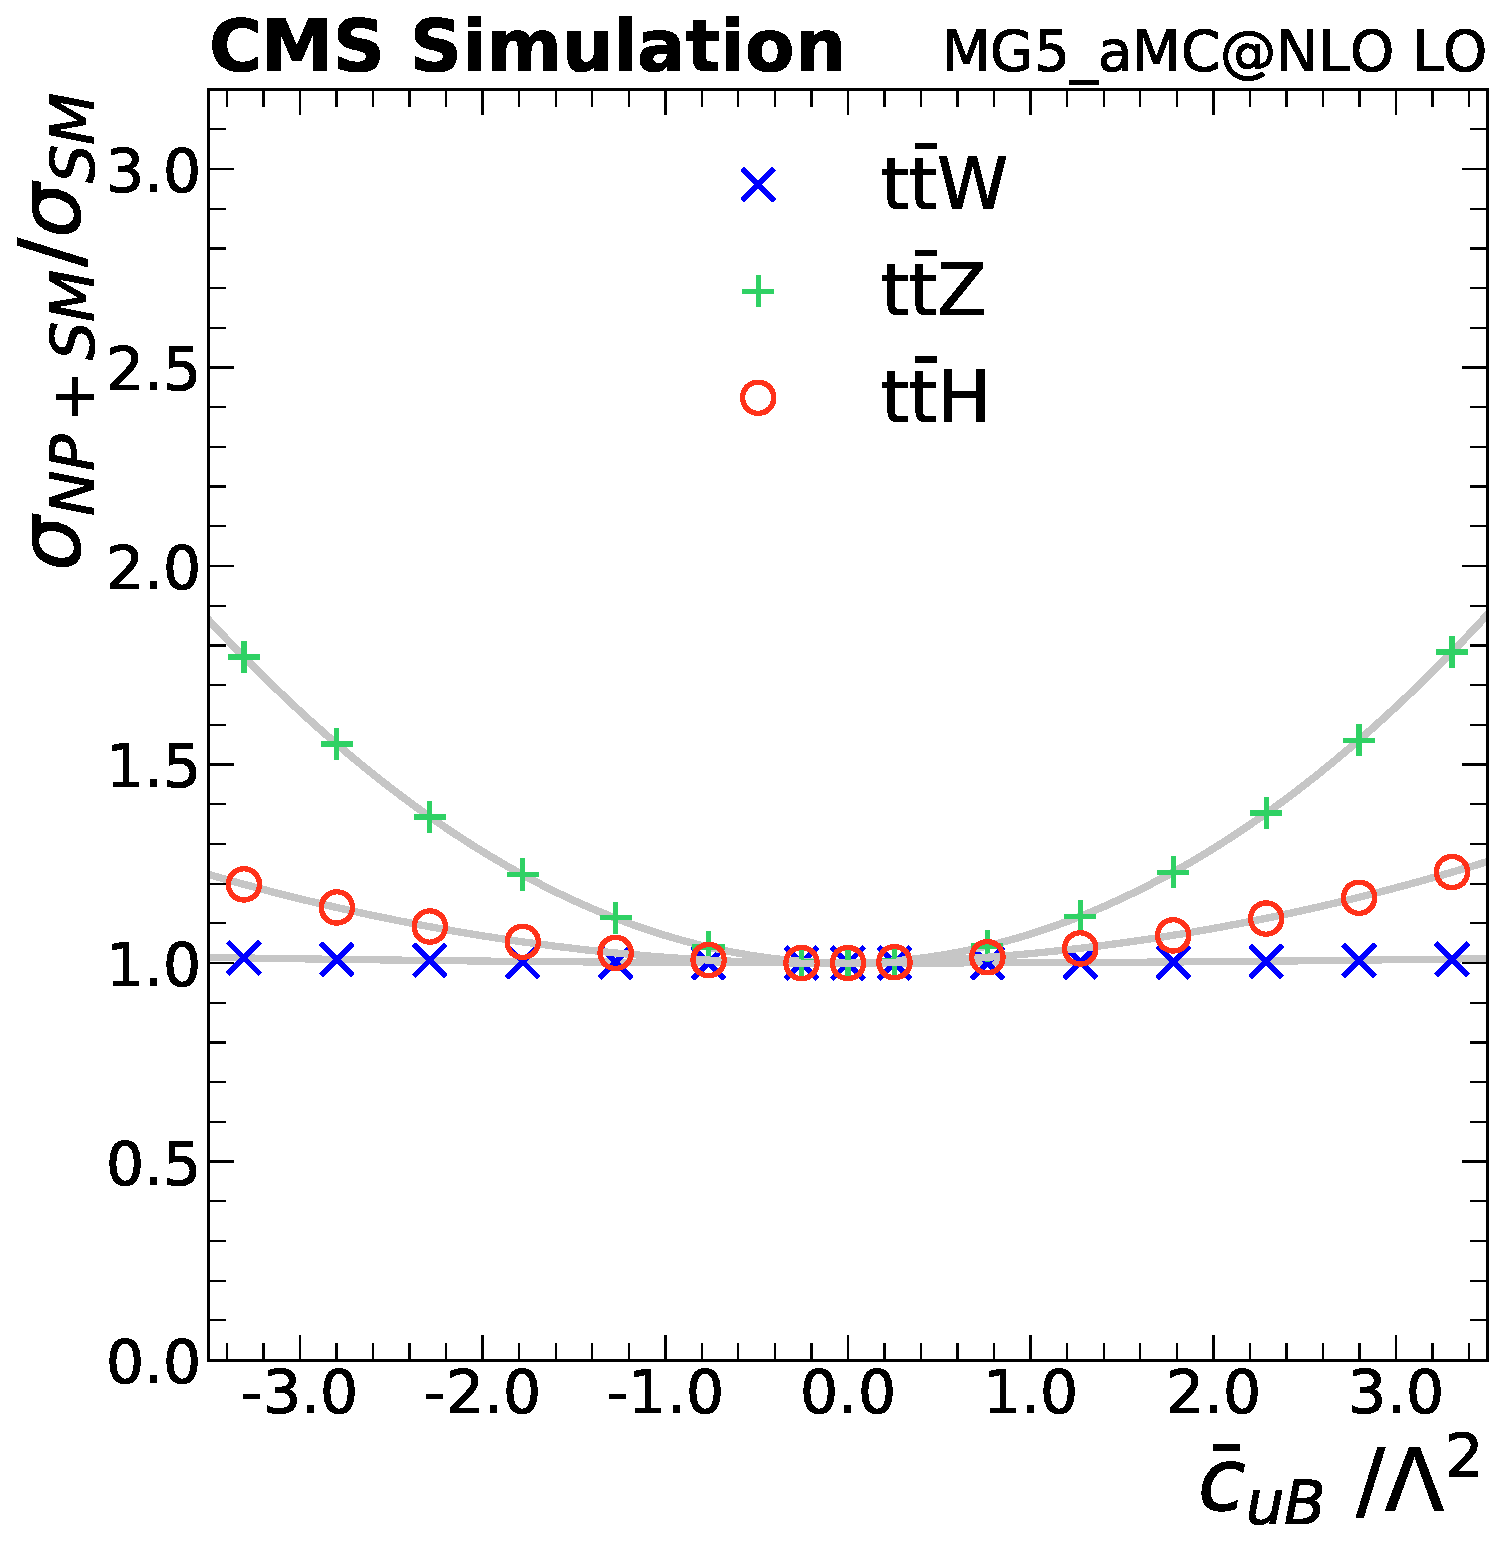
\includegraphics[height=\textheight]{figures/thirteen-TeV/NP/mu/cuB}\hspace{1cm}
        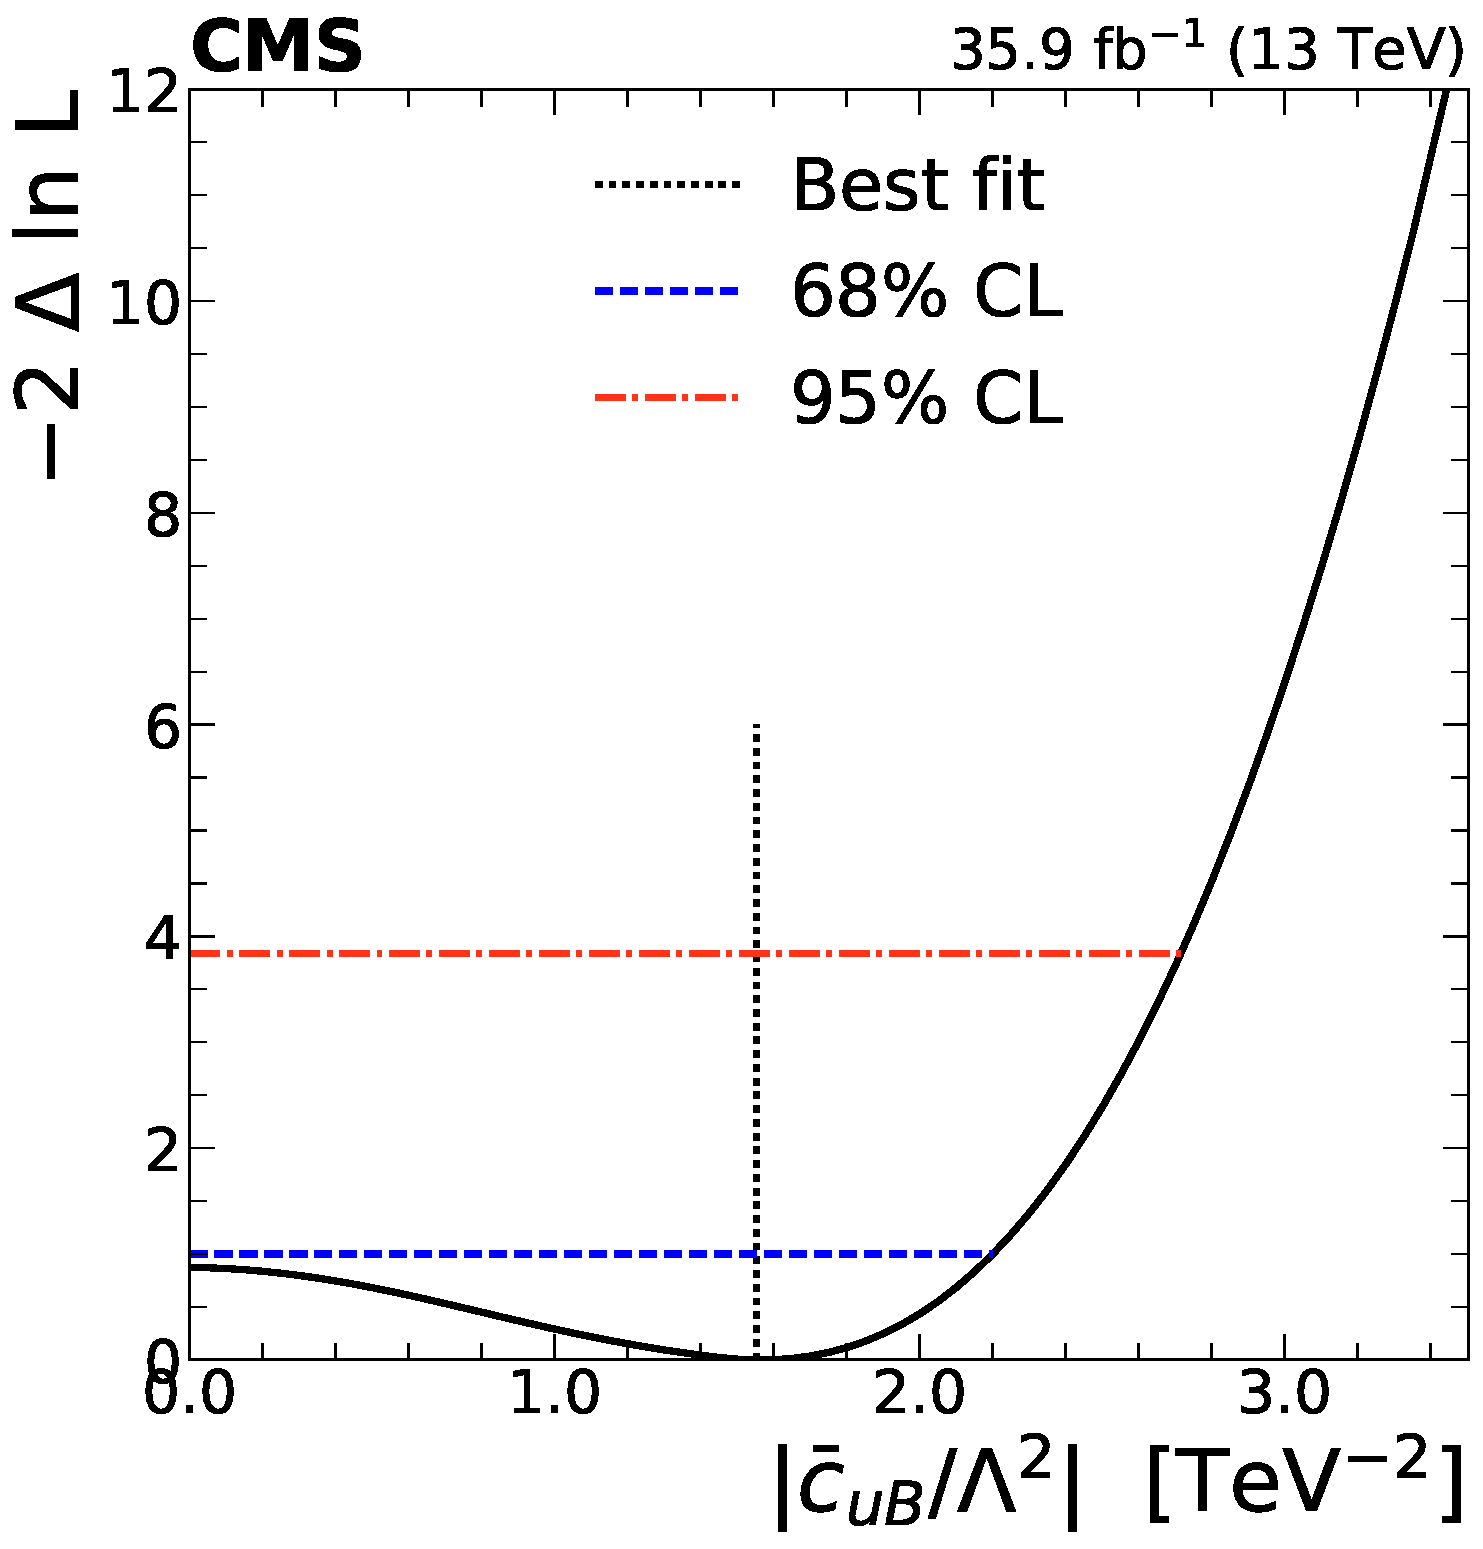
\includegraphics[height=\textheight]{figures/thirteen-TeV/NP/nll/cuB}\hspace{1cm}
        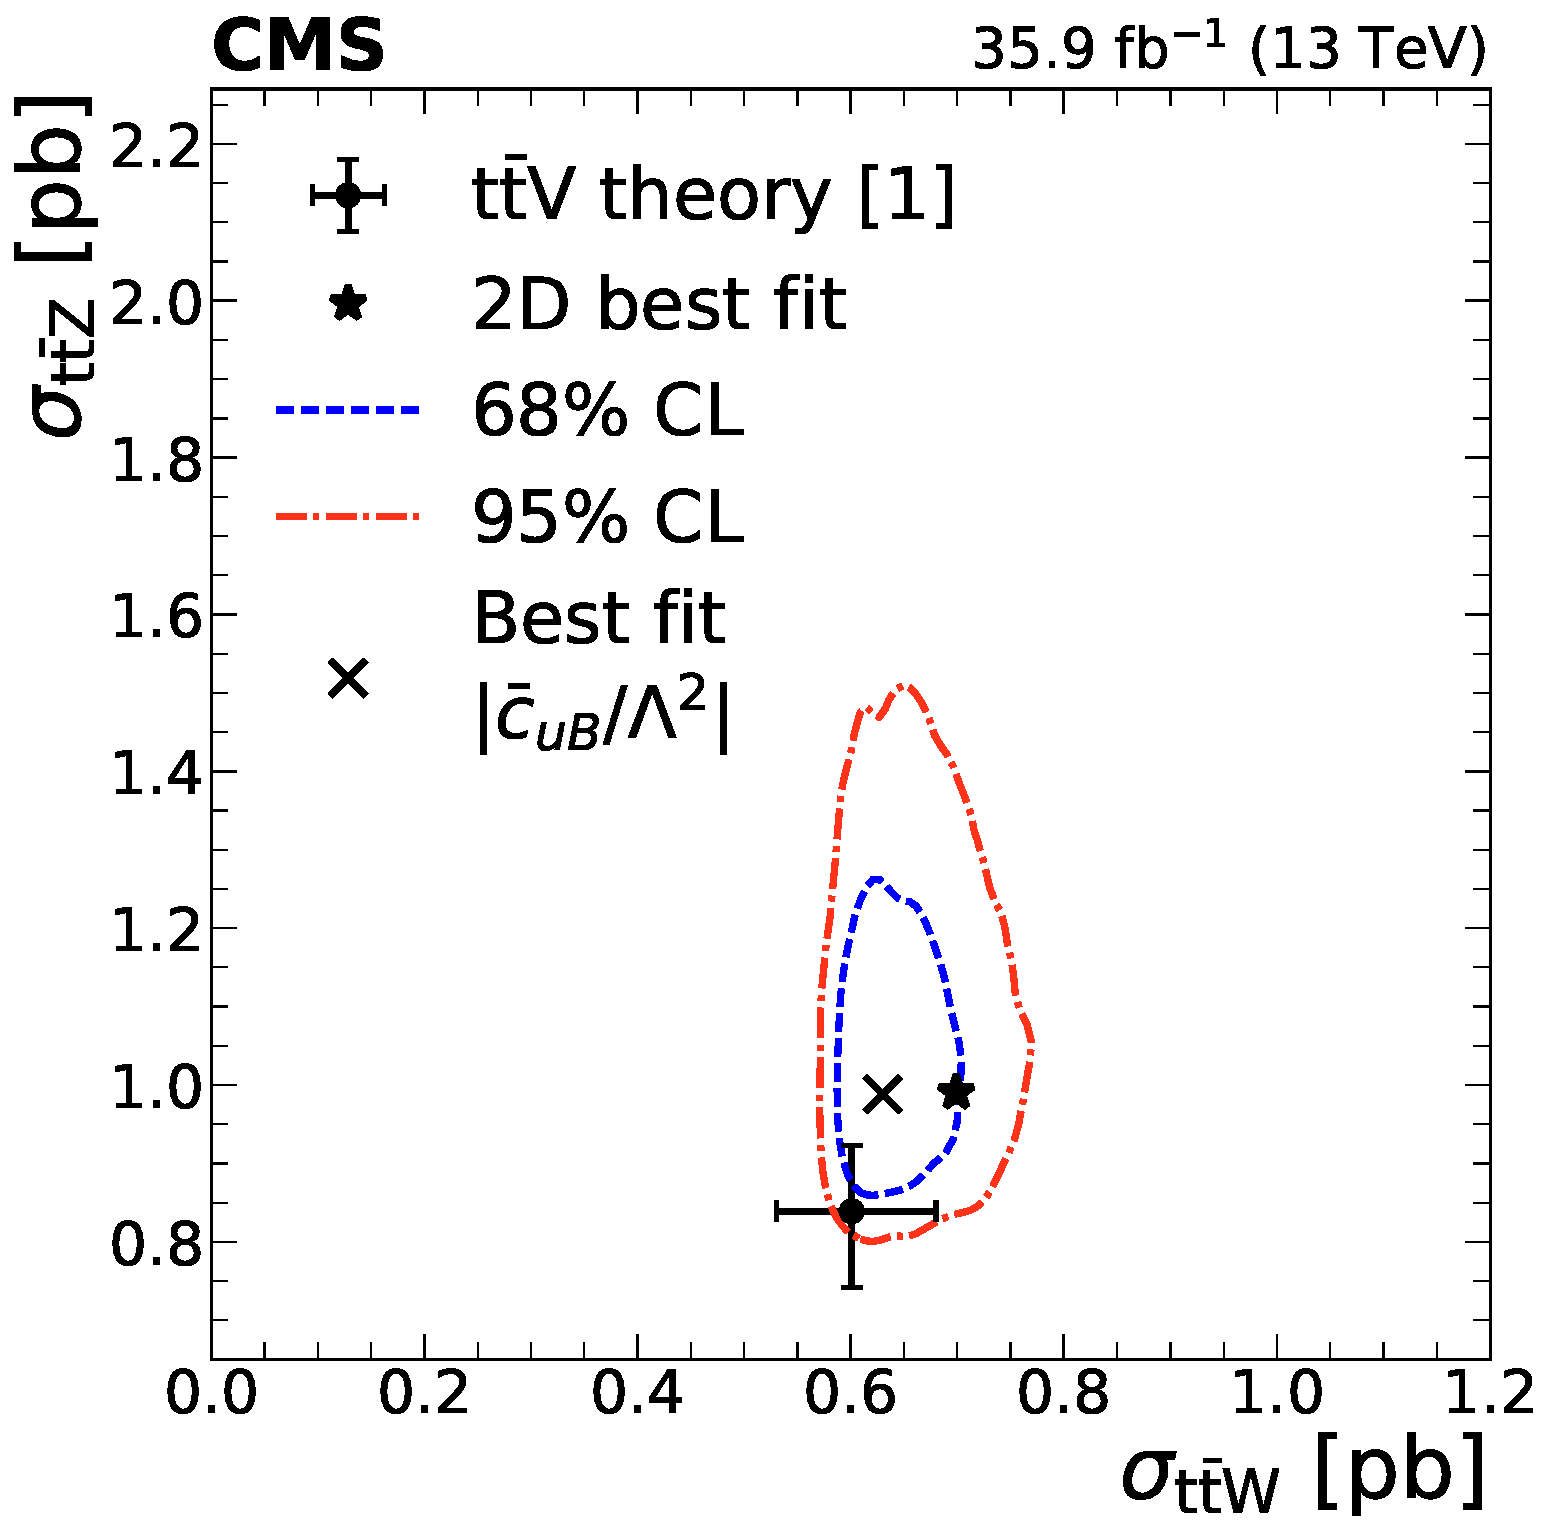
\includegraphics[height=\textheight]{figures/thirteen-TeV/NP/2D/ttZ_ttW_2D_1D_cuB}
      }
    \setlength{\capwidth}{14cm}
    \caption[Profile likelihood, $\mu(c_1)$, and best fit $c_1$ for \cuB (\thirteenTeV)]{Left: signal scaling as a function of the $c_1$ for \ttW (crosses), \ttZ (pluses), and \ttH (circles) for \cuB (\thirteenTeV analysis). Center: the test statistic $q(c_i)$ scan as a function of $c_1$, profiling all other nuisance parameters. The best fit value is indicated by a dotted line. Dashed and dash-dotted lines indicate \SI{68}{\percent} and \SI{95}{\percent} CL intervals, respectively. Right: The best fit $c_1$ value (shown as a cross), along with the corresponding \SI{68}{\percent} (dashed) and \SI{95}{\percent} (dash-dotted) contours in the $\sigma_{\ttZ}, \sigma_{\ttW}$ plane. The two-dimensional best fit to the \ttW and \ttZ cross sections is given by the star. The theory predictions~\cite{deFlorian:2016spz} are shown as a dot with bars representing their respective uncertainties.}
    \label{fig:results-cuB}
  \end{figure}
  \begin{figure}
      \resizebox{!}{7.2cm}{
        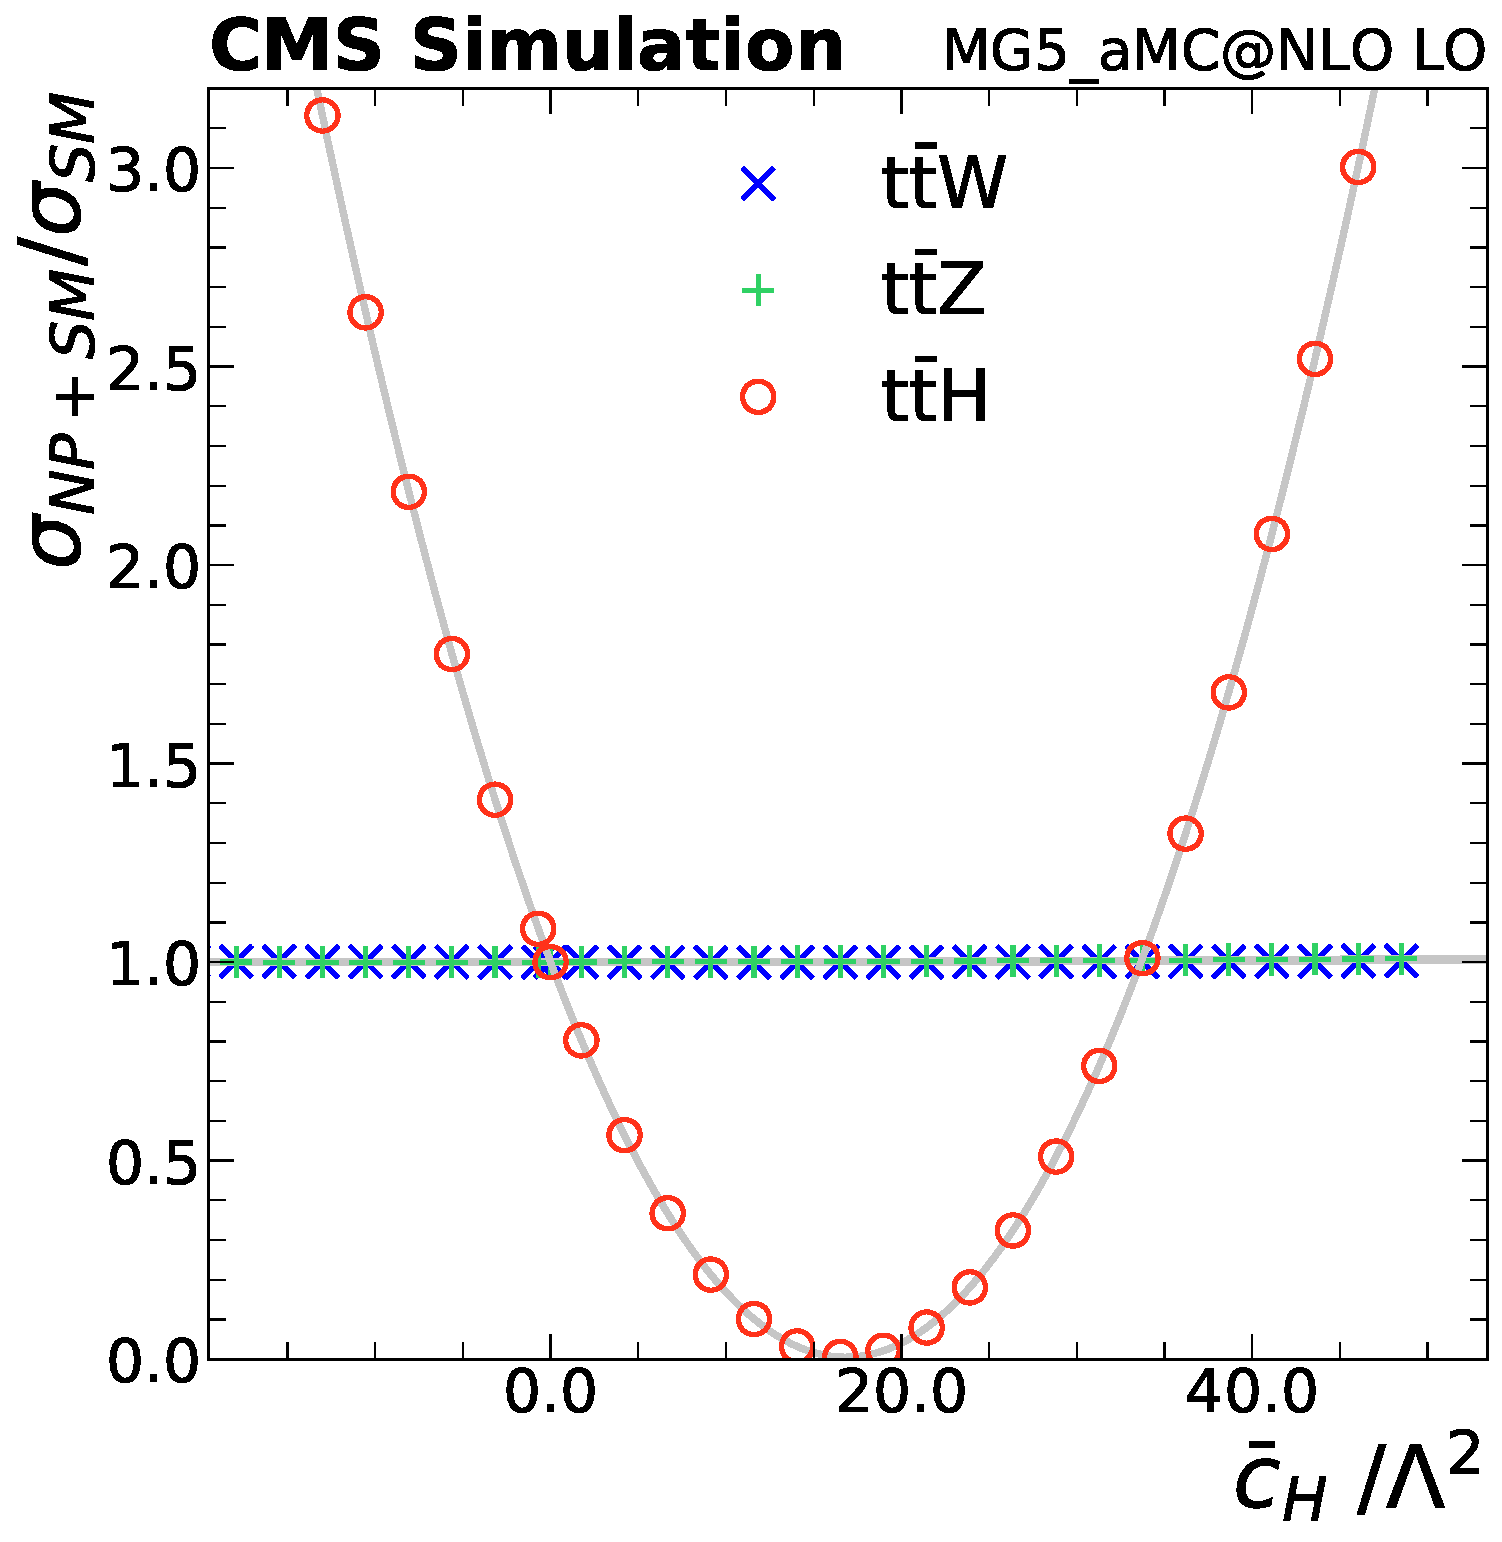
\includegraphics[height=\textheight]{figures/thirteen-TeV/NP/mu/cH}\hspace{1cm}
        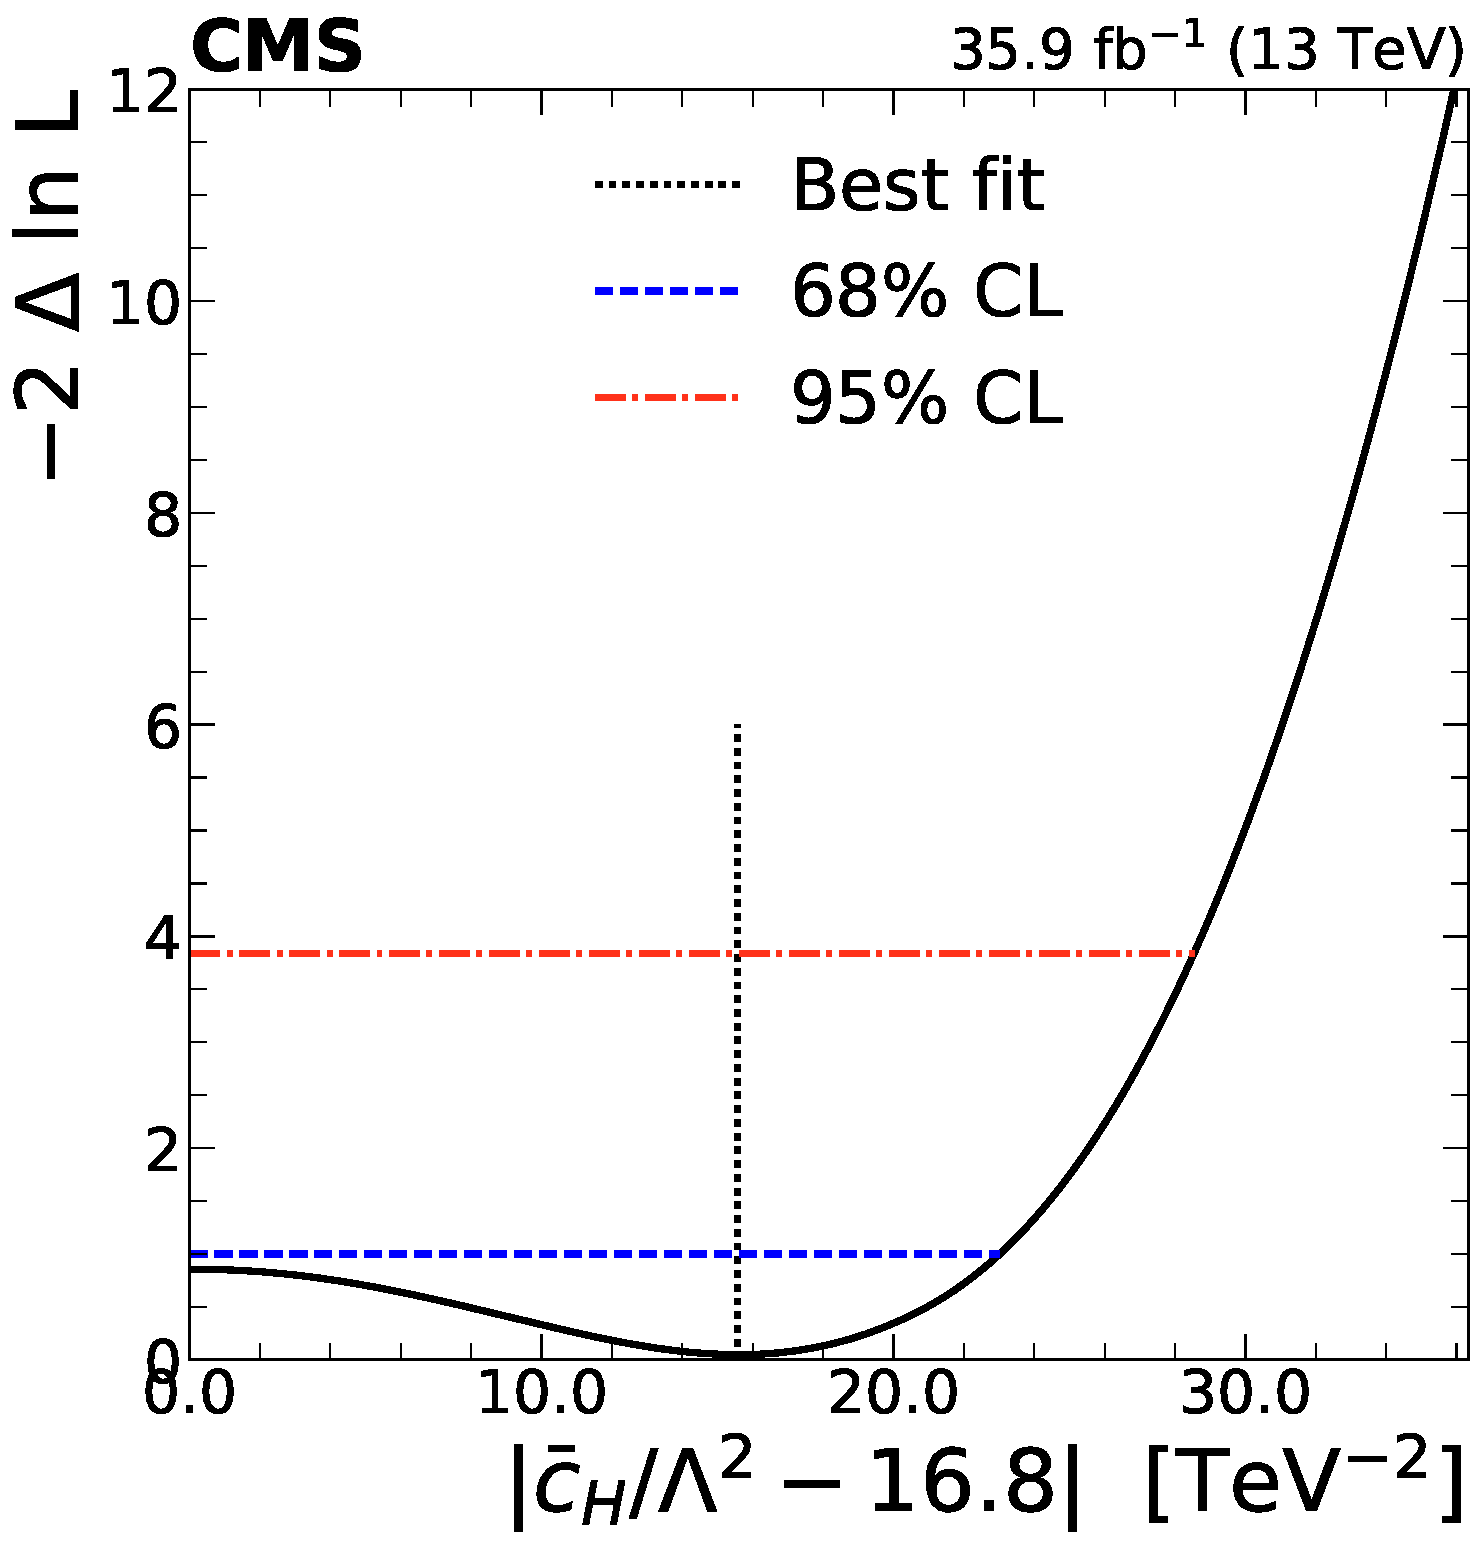
\includegraphics[height=\textheight]{figures/thirteen-TeV/NP/nll/cH}\hspace{1cm}
        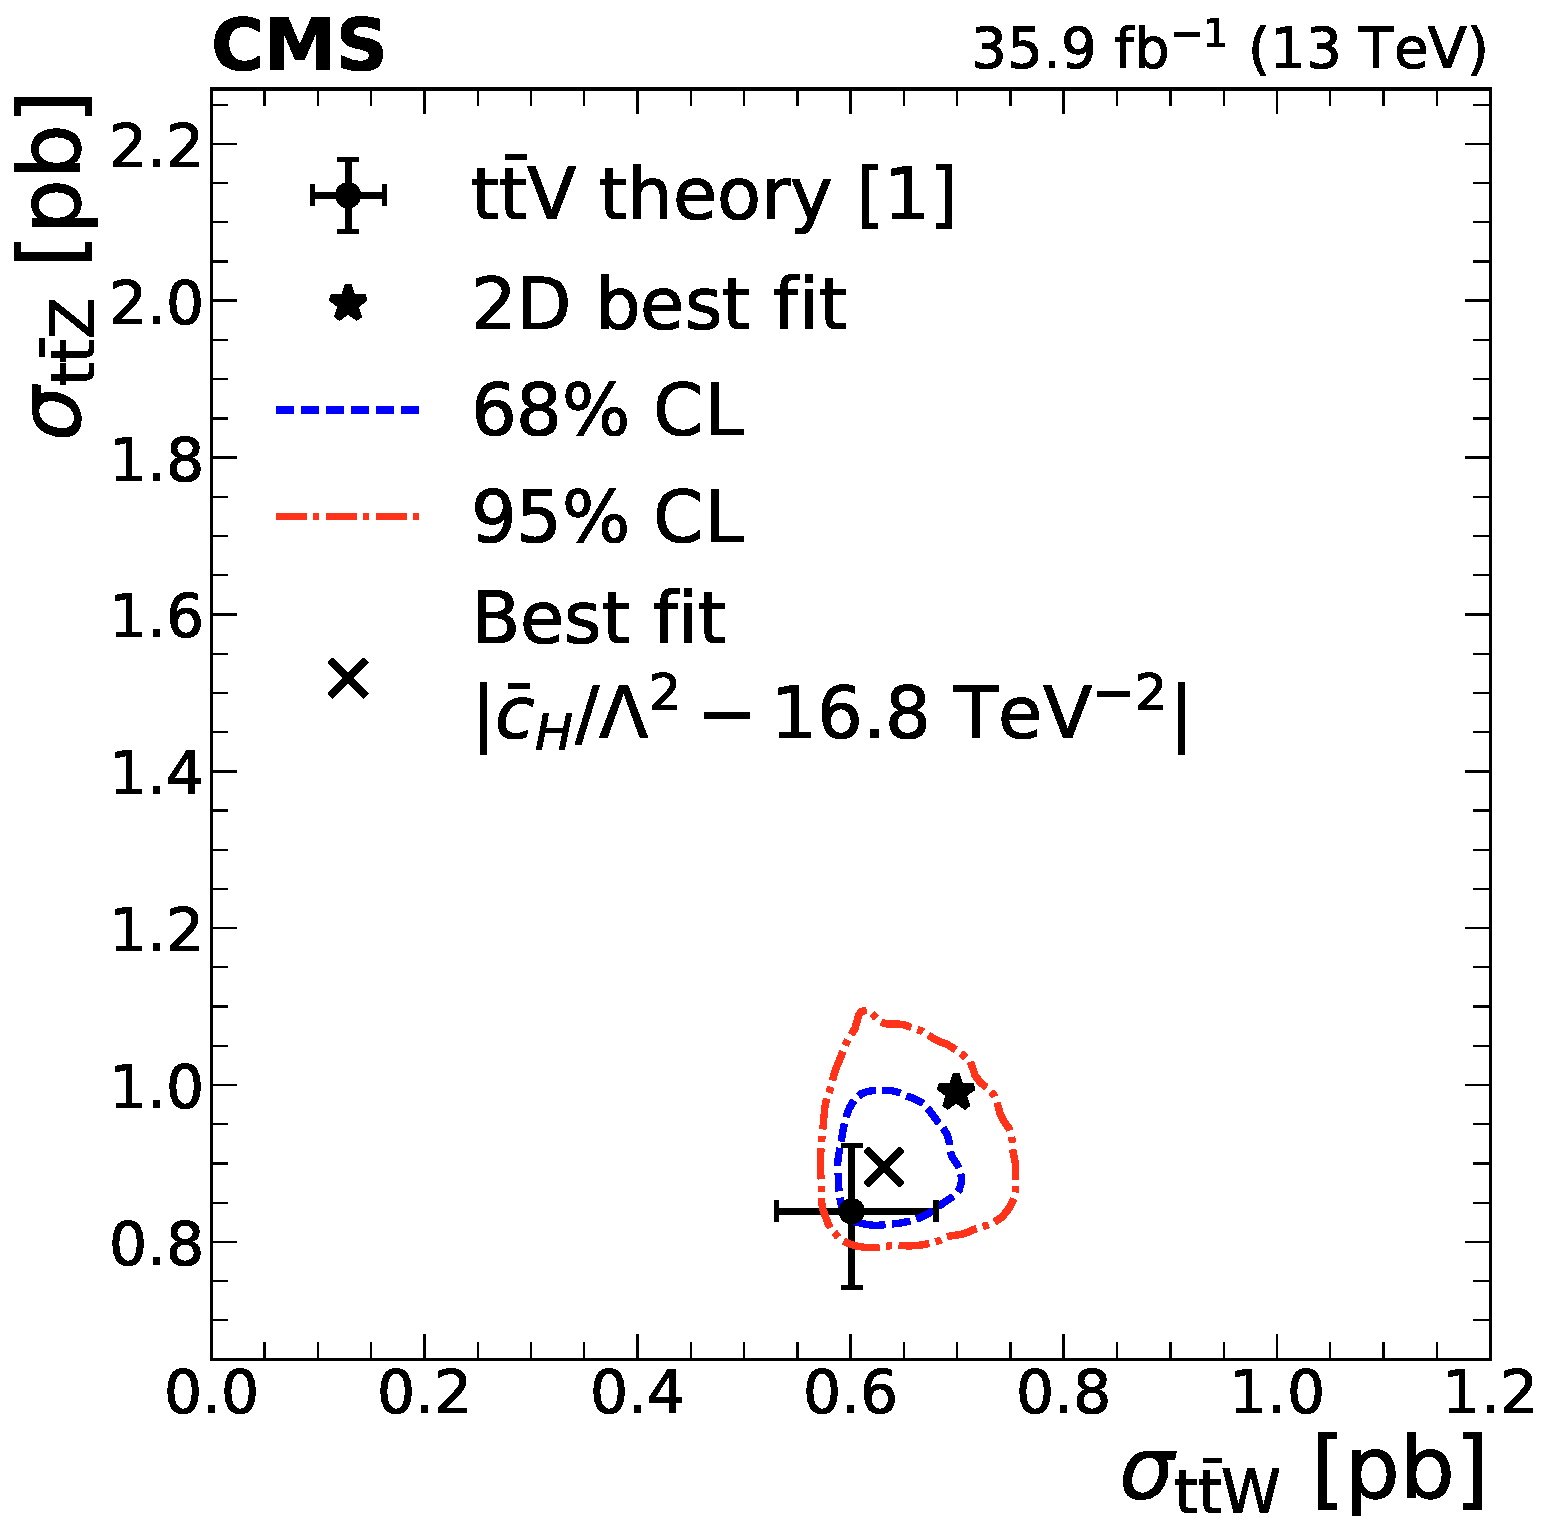
\includegraphics[height=\textheight]{figures/thirteen-TeV/NP/2D/ttZ_ttW_2D_1D_cH}
      }
    \setlength{\capwidth}{14cm}
    \caption[Profile likelihood, $\mu(c_1)$, and best fit $c_1$ for \cH (\thirteenTeV)]{Left: signal scaling as a function of the $c_1$ for \ttW (crosses), \ttZ (pluses), and \ttH (circles) for \cH (\thirteenTeV analysis). Center: the test statistic $q(c_i)$ scan as a function of $c_1$, profiling all other nuisance parameters. The best fit value is indicated by a dotted line. Dashed and dash-dotted lines indicate \SI{68}{\percent} and \SI{95}{\percent} CL intervals, respectively. Right: The best fit $c_1$ value (shown as a cross), along with the corresponding \SI{68}{\percent} (dashed) and \SI{95}{\percent} (dash-dotted) contours in the $\sigma_{\ttZ}, \sigma_{\ttW}$ plane. The two-dimensional best fit to the \ttW and \ttZ cross sections is given by the star. The theory predictions~\cite{deFlorian:2016spz} are shown as a dot with bars representing their respective uncertainties.}
    \label{fig:results-cH}
  \end{figure}
  \begin{figure}
      \centering
      \resizebox{!}{7.2cm}{
        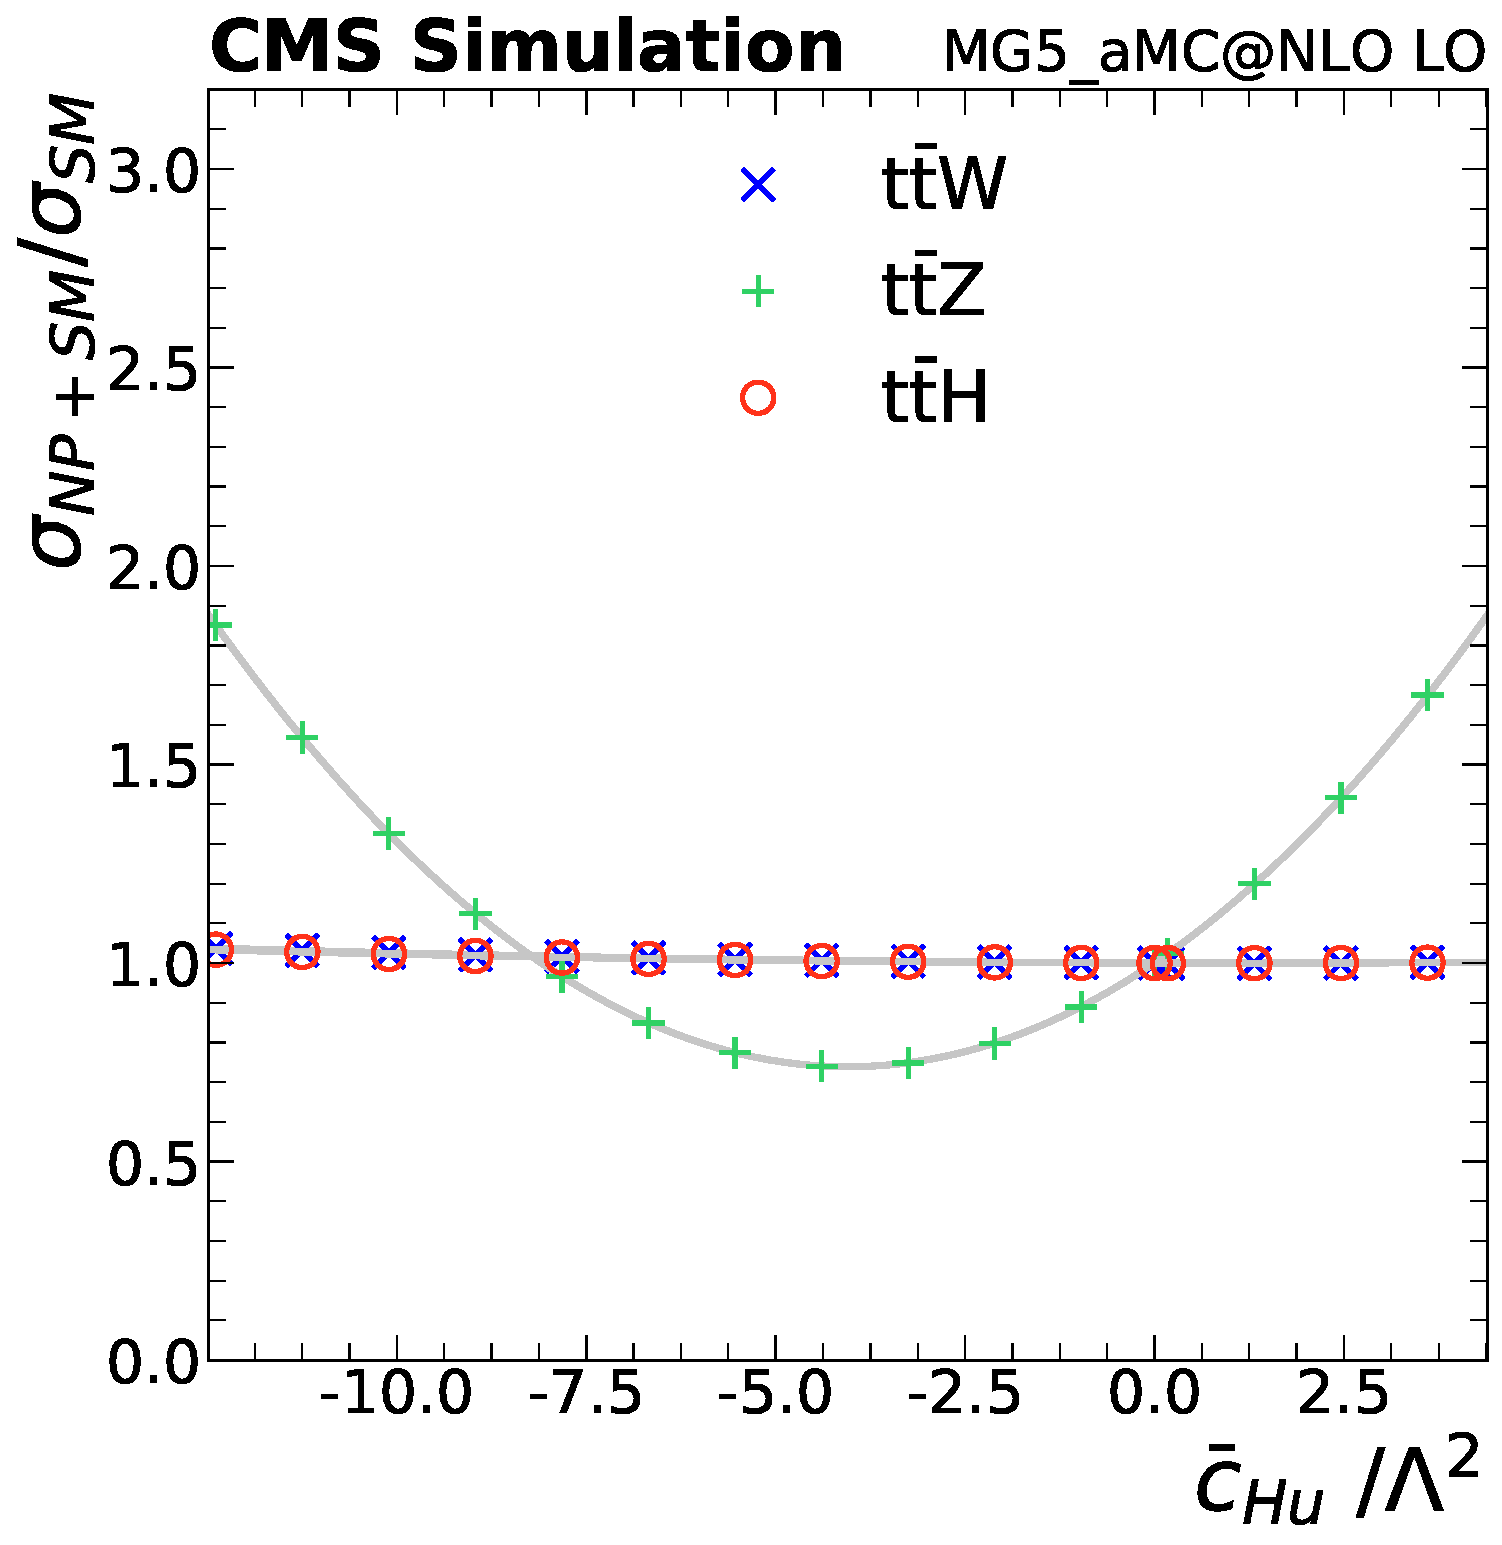
\includegraphics[height=\textheight]{figures/thirteen-TeV/NP/mu/cHu}\hspace{1cm}
        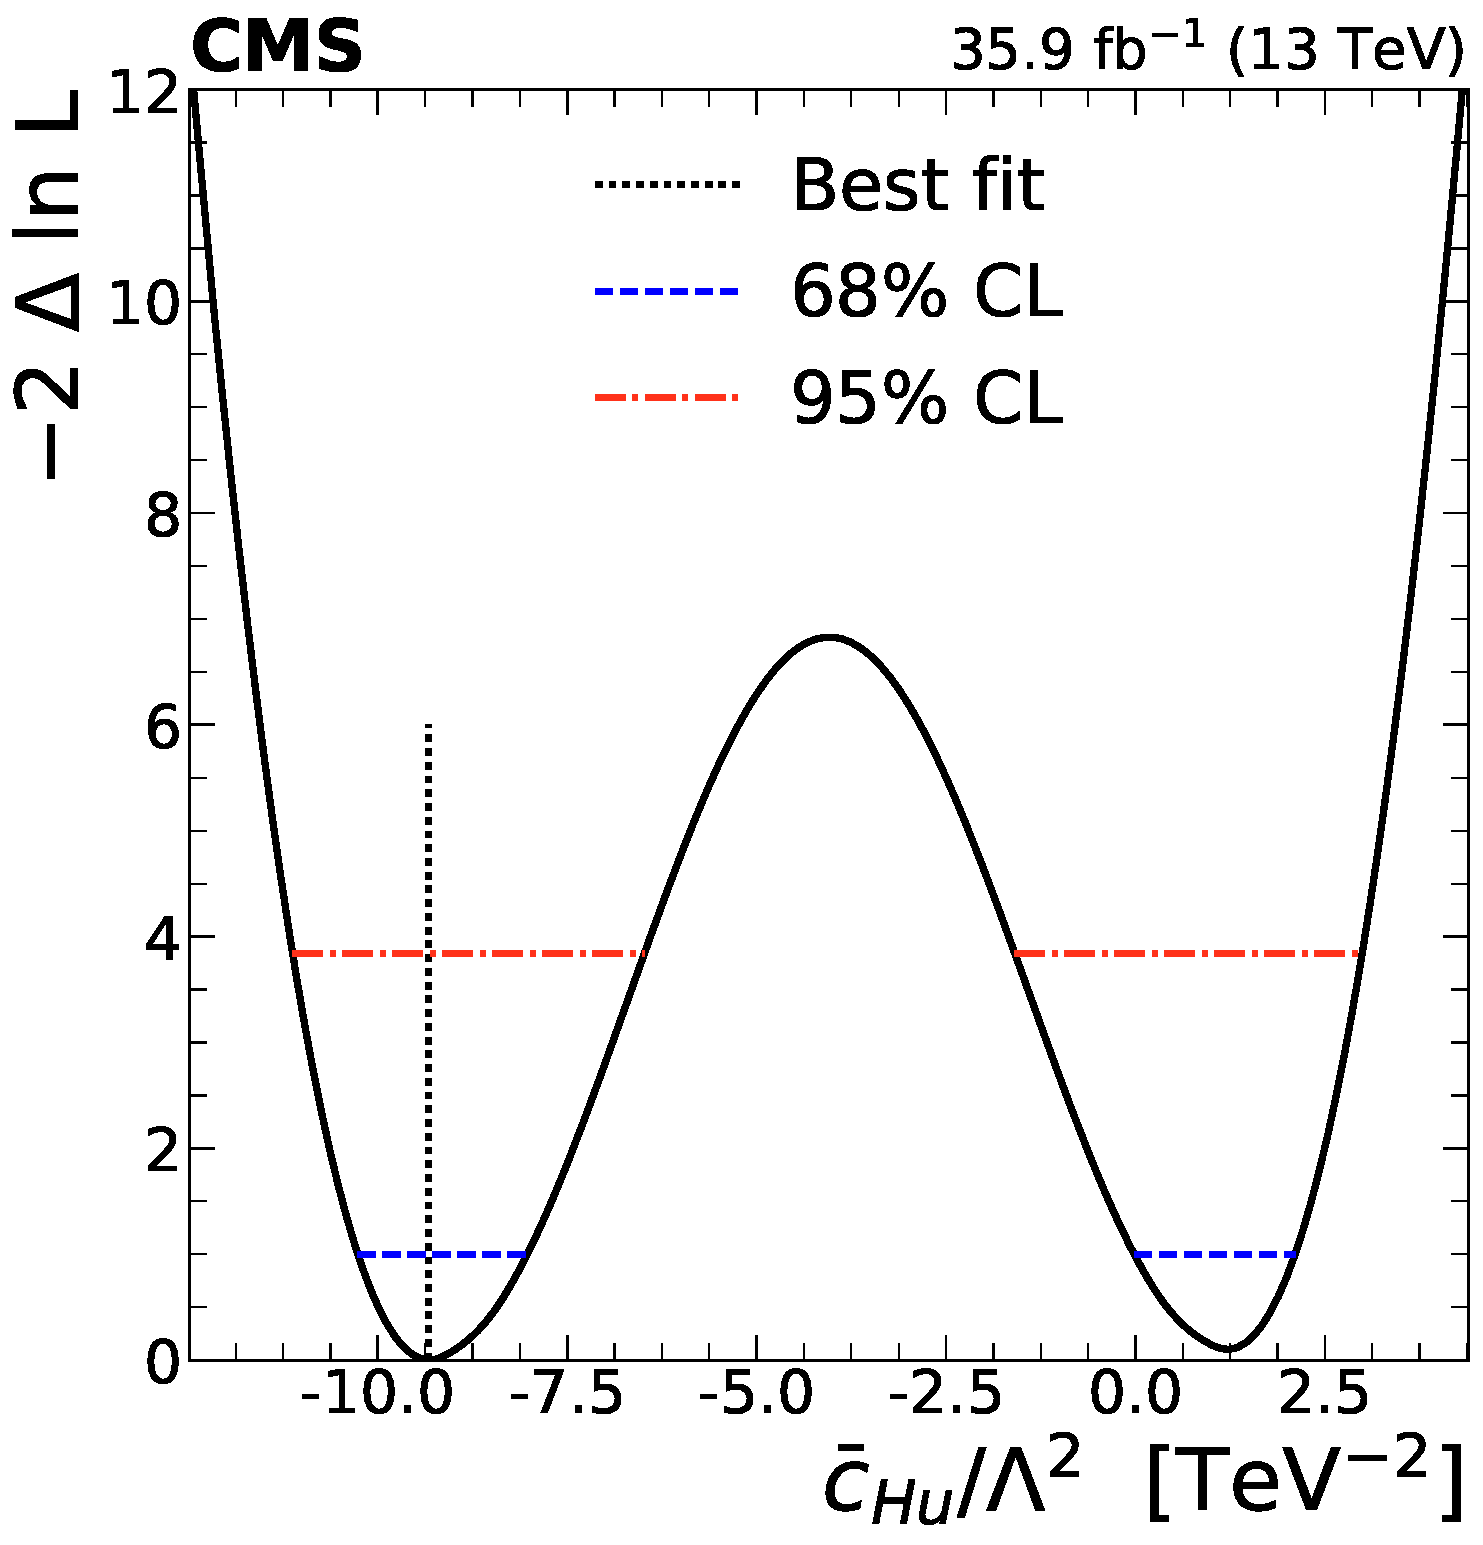
\includegraphics[height=\textheight]{figures/thirteen-TeV/NP/nll/cHu}\hspace{1cm}
        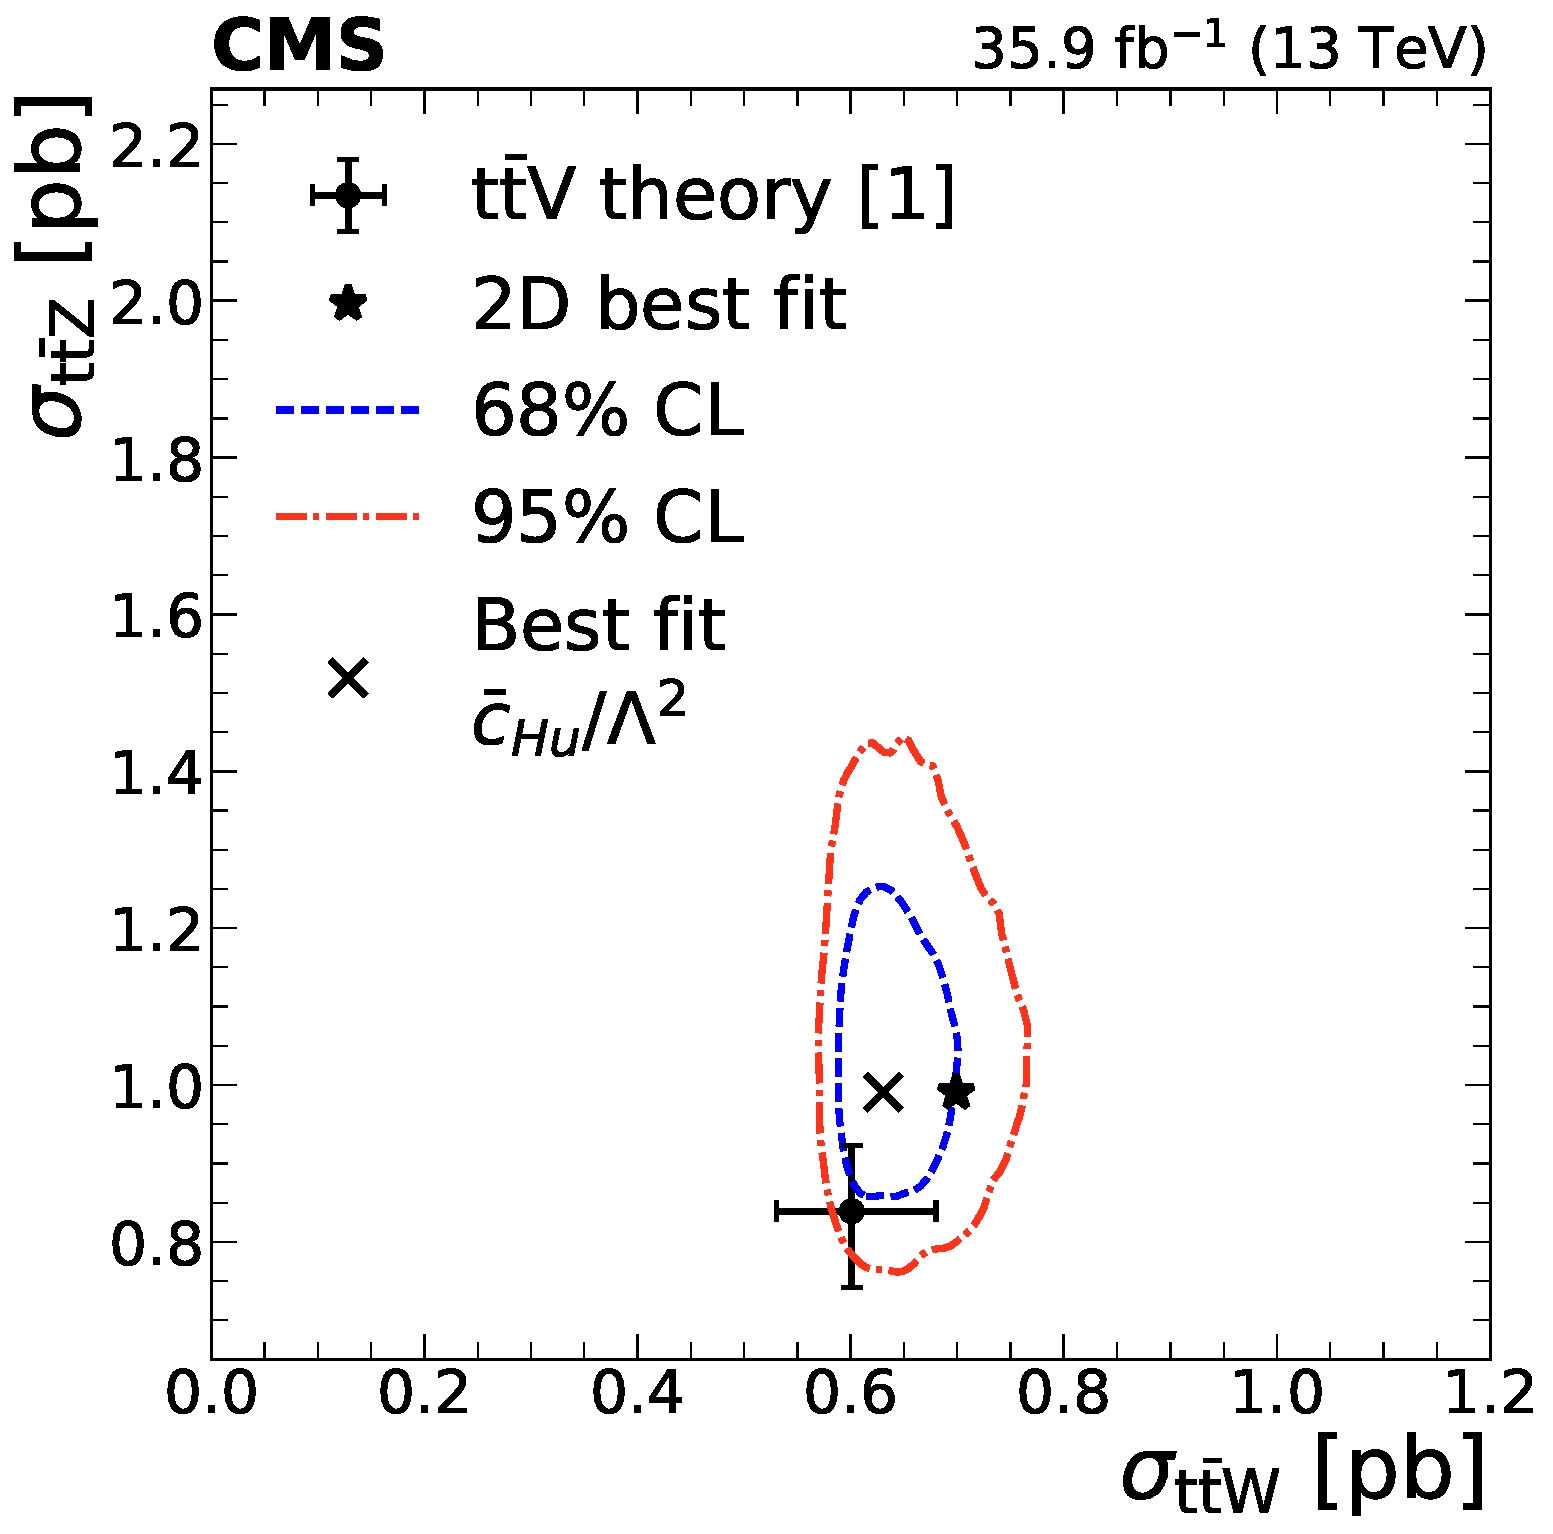
\includegraphics[height=\textheight]{figures/thirteen-TeV/NP/2D/ttZ_ttW_2D_1D_cHu}
      }
    \setlength{\capwidth}{14cm}
    \caption[Profile likelihood, $\mu(c_1)$, and best fit $c_1$ for \cHu (\thirteenTeV)]{Left: signal scaling as a function of the $c_1$ for \ttW (crosses), \ttZ (pluses), and \ttH (circles) for \cHu (\thirteenTeV analysis). Center: the test statistic $q(c_i)$ scan as a function of $c_1$, profiling all other nuisance parameters. The best fit value is indicated by a dotted line. Dashed and dash-dotted lines indicate \SI{68}{\percent} and \SI{95}{\percent} CL intervals, respectively. Right: The best fit $c_1$ value (shown as a cross), along with the corresponding \SI{68}{\percent} (dashed) and \SI{95}{\percent} (dash-dotted) contours in the $\sigma_{\ttZ}, \sigma_{\ttW}$ plane. The two-dimensional best fit to the \ttW and \ttZ cross sections is given by the star. The theory predictions~\cite{deFlorian:2016spz} are shown as a dot with bars representing their respective uncertainties.}
    \label{fig:results-cHu}
  \end{figure}
\end{landscape}

\begin{table}
  \input{tables/thirteen-TeV/1d-expected-CLs}
\end{table}
\begin{table}
  \input{tables/thirteen-TeV/1d-CLs}
\end{table}

\begin{table}
  \input{tables/thirteen-TeV/scaling}
\end{table}

\begin{figure}
  \begin{subfigure}{\linewidth}
    \centering
    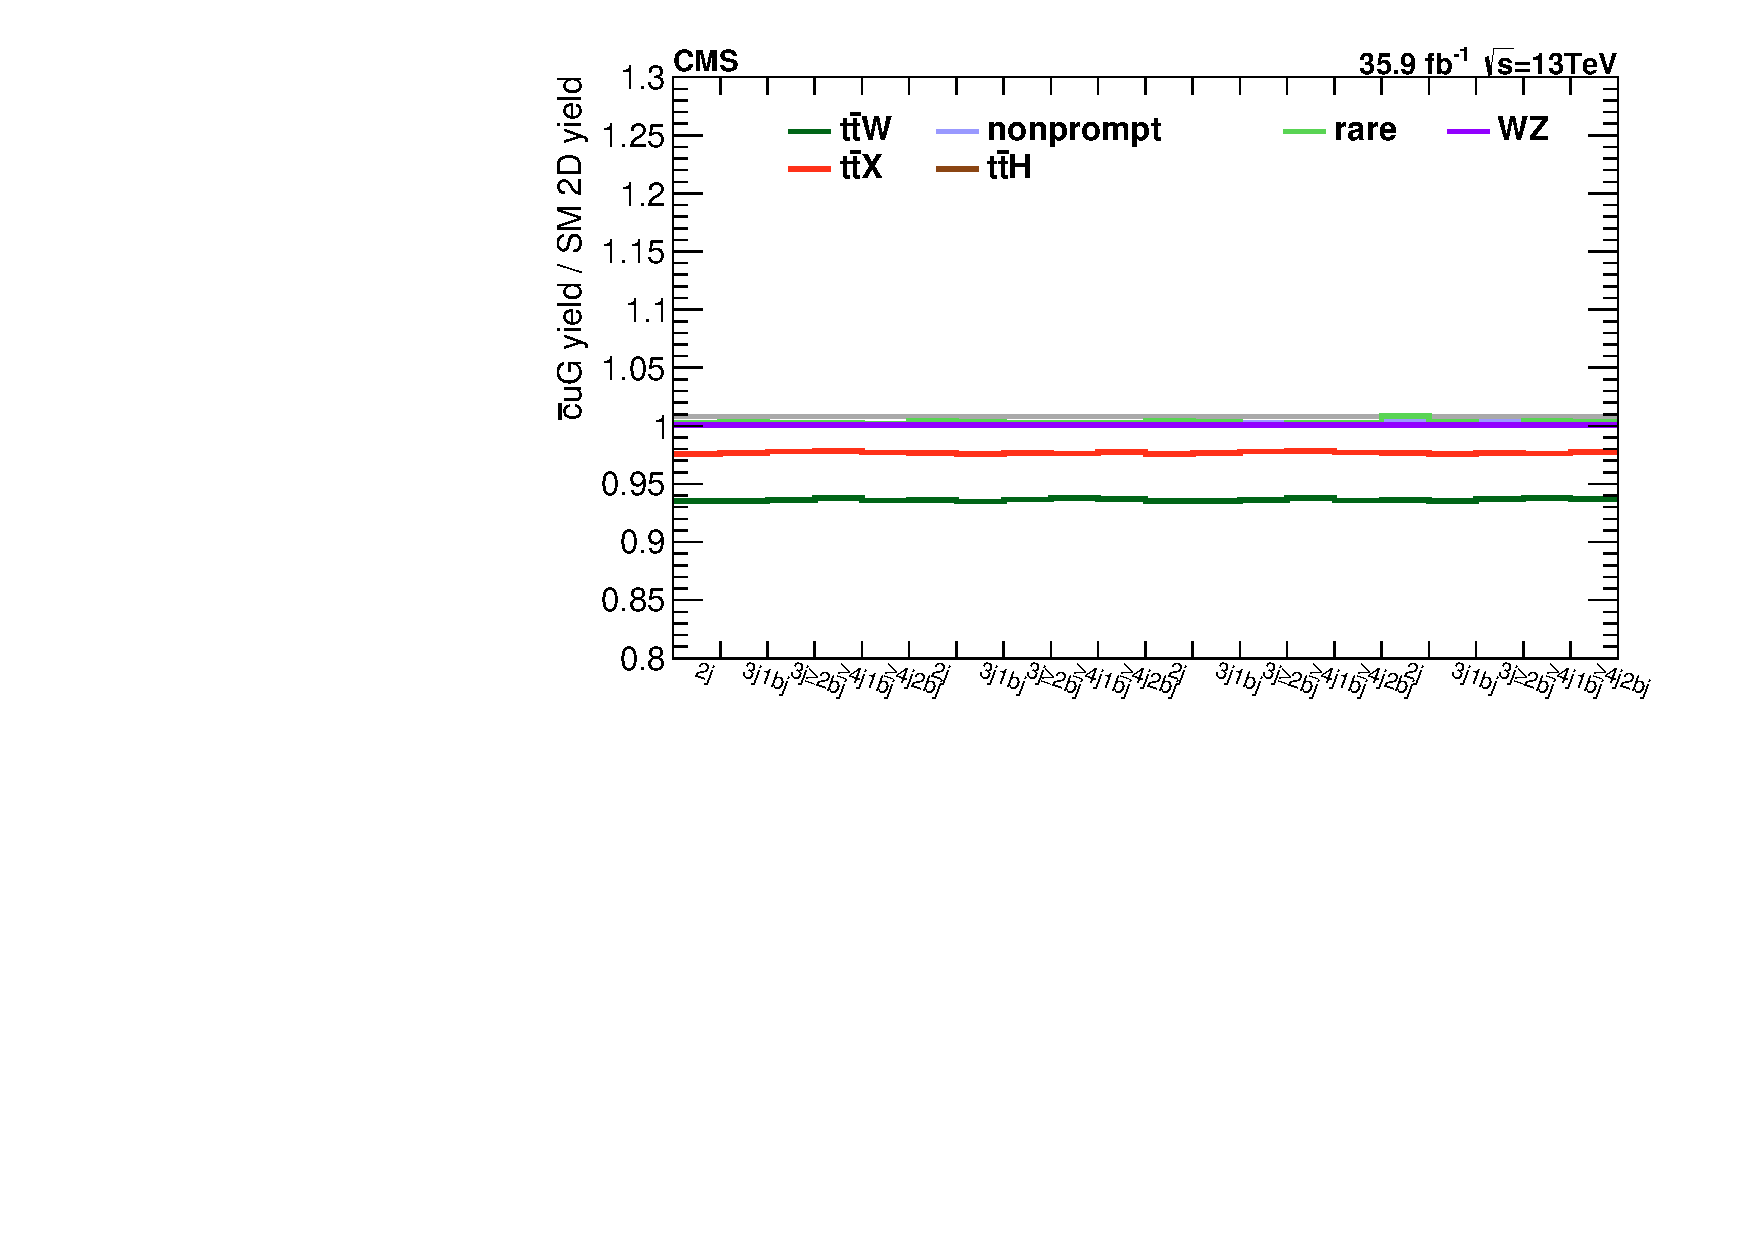
\includegraphics[width=0.5\textwidth]{figures/thirteen-TeV/postfit/ratio_2l_cuG}%
    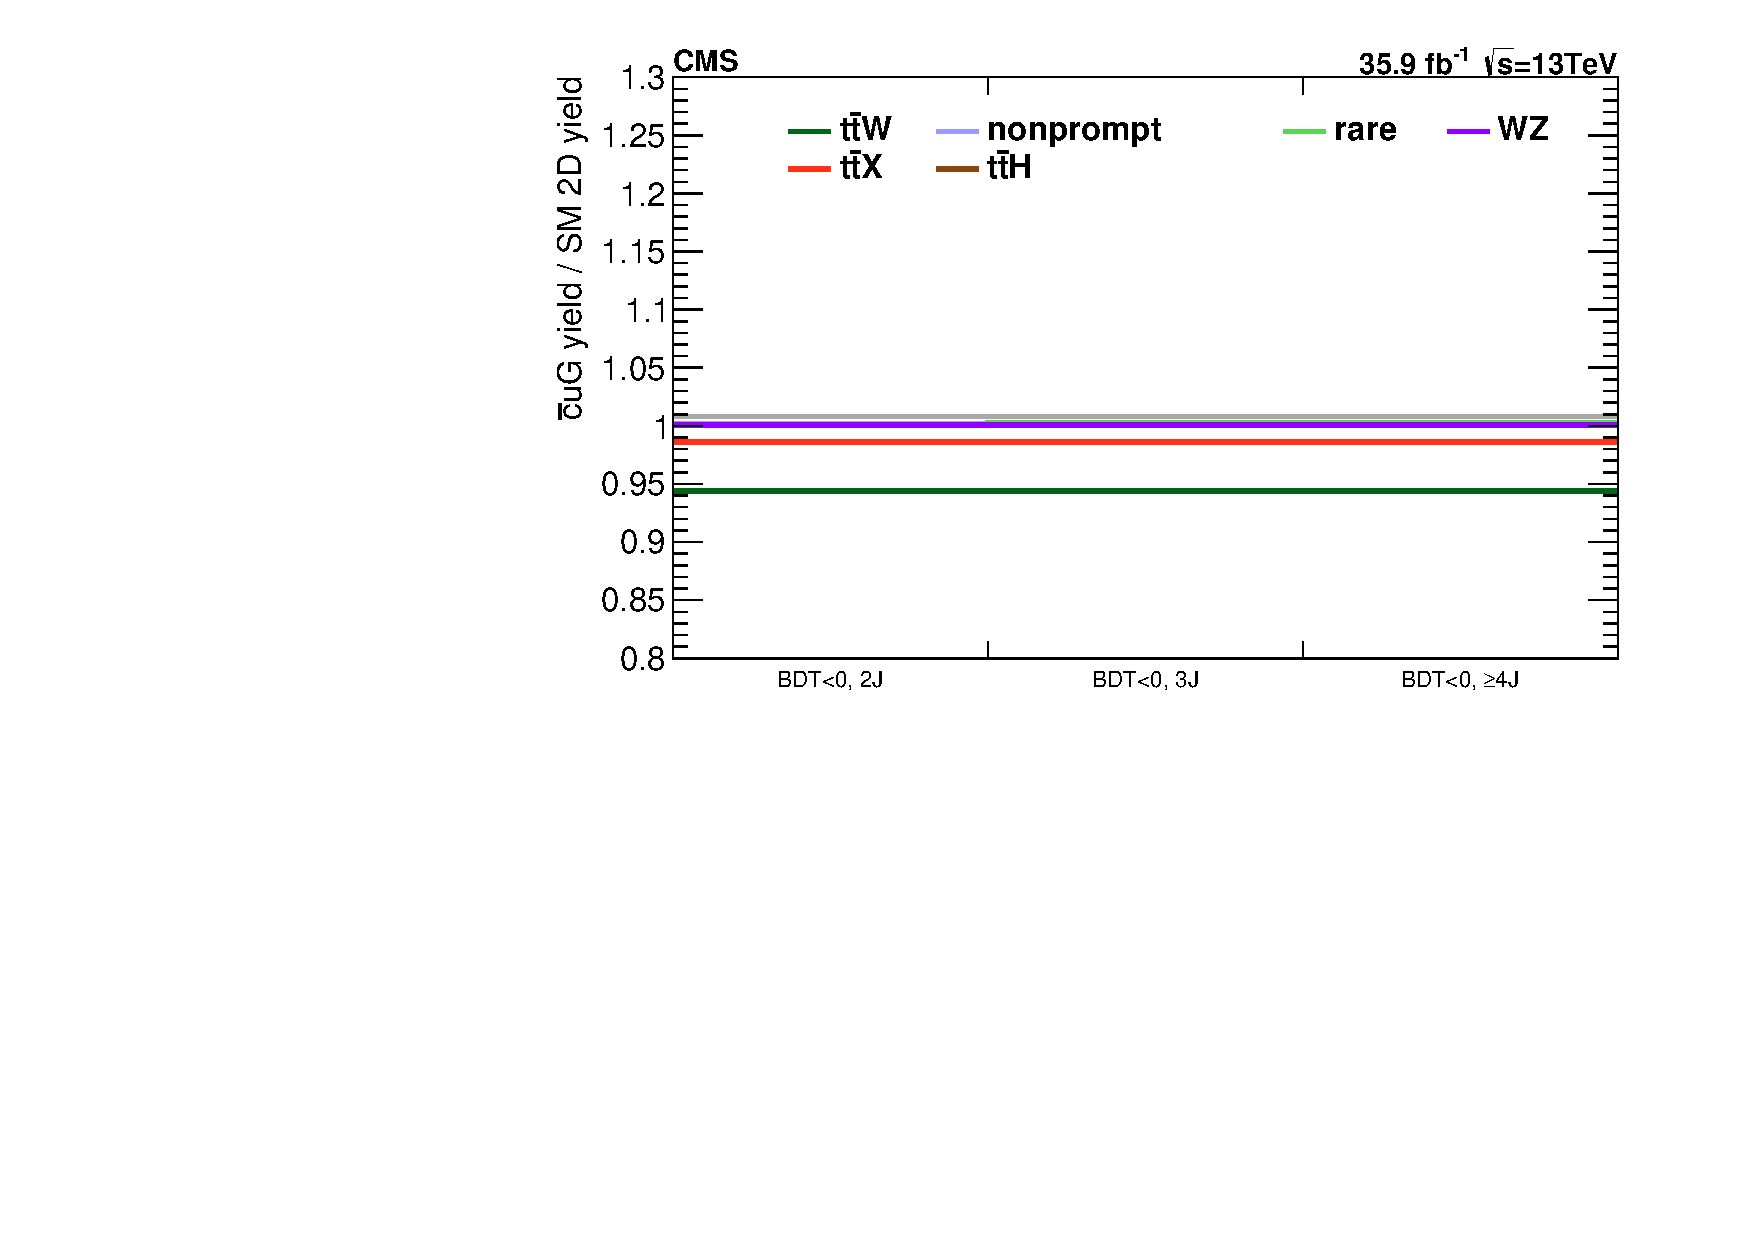
\includegraphics[width=0.5\textwidth]{figures/thirteen-TeV/postfit/ratio_2l-cr_cuG}
    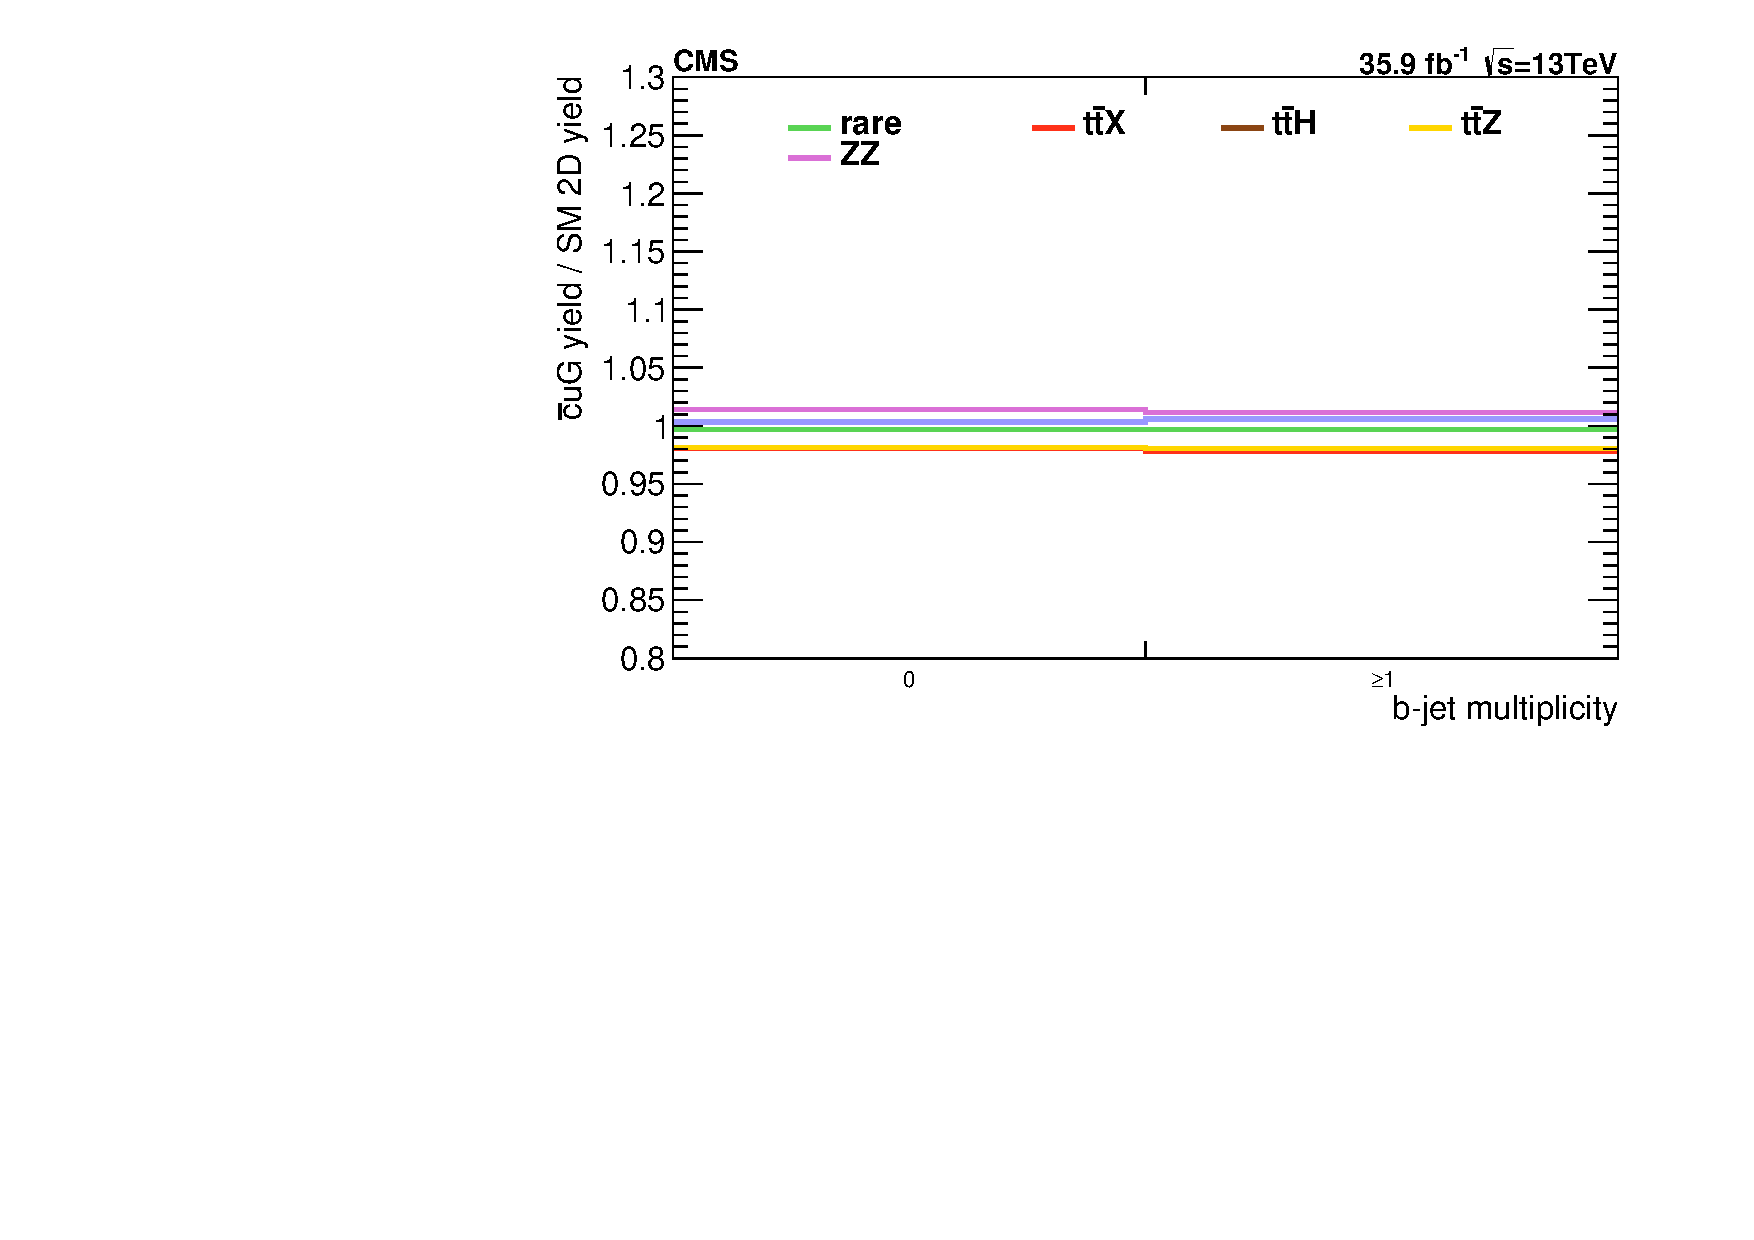
\includegraphics[width=0.5\textwidth]{figures/thirteen-TeV/postfit/ratio_4l_cuG}%
    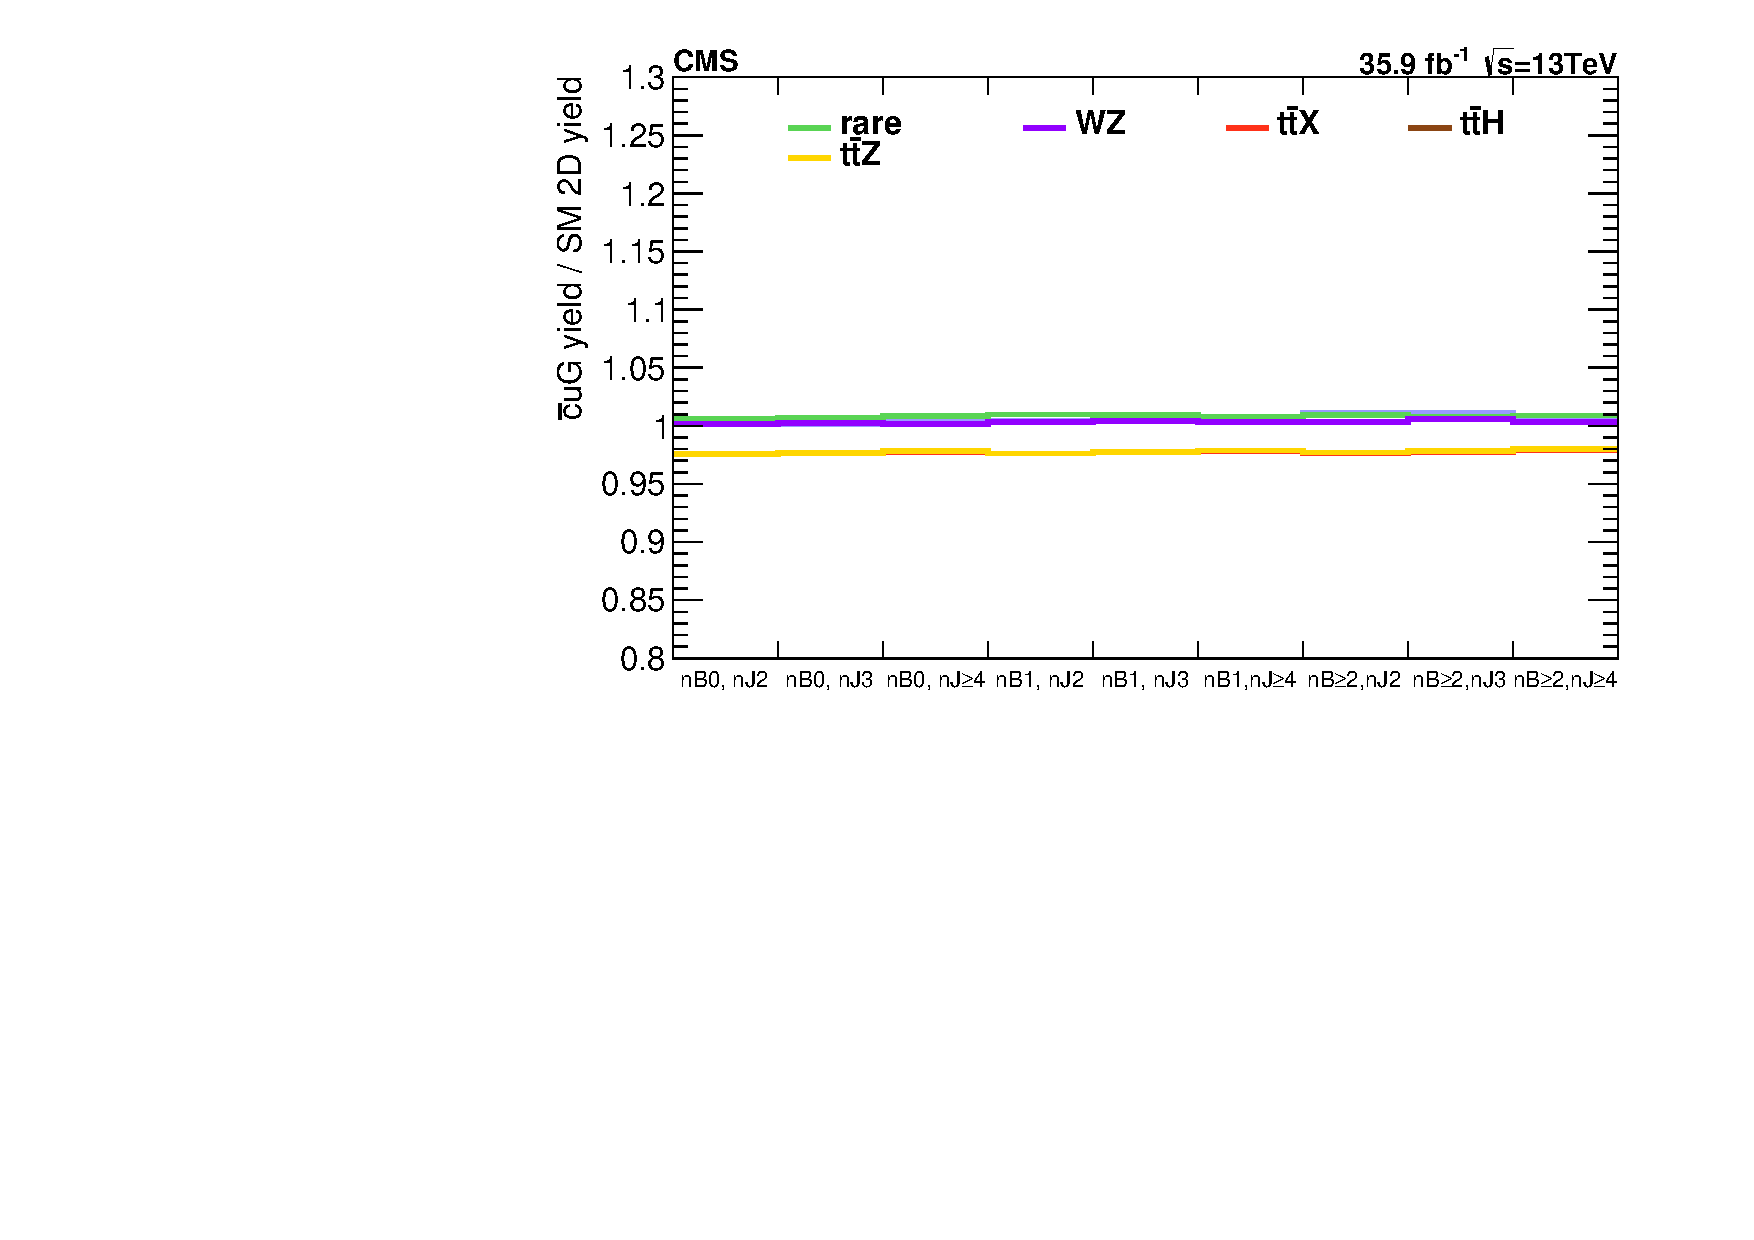
\includegraphics[width=0.5\textwidth]{figures/thirteen-TeV/postfit/ratio_3l_cuG}
    \caption{}
    \label{sfig:ratio-cuG}
  \end{subfigure}
  \begin{subfigure}{\linewidth}
    \centering
    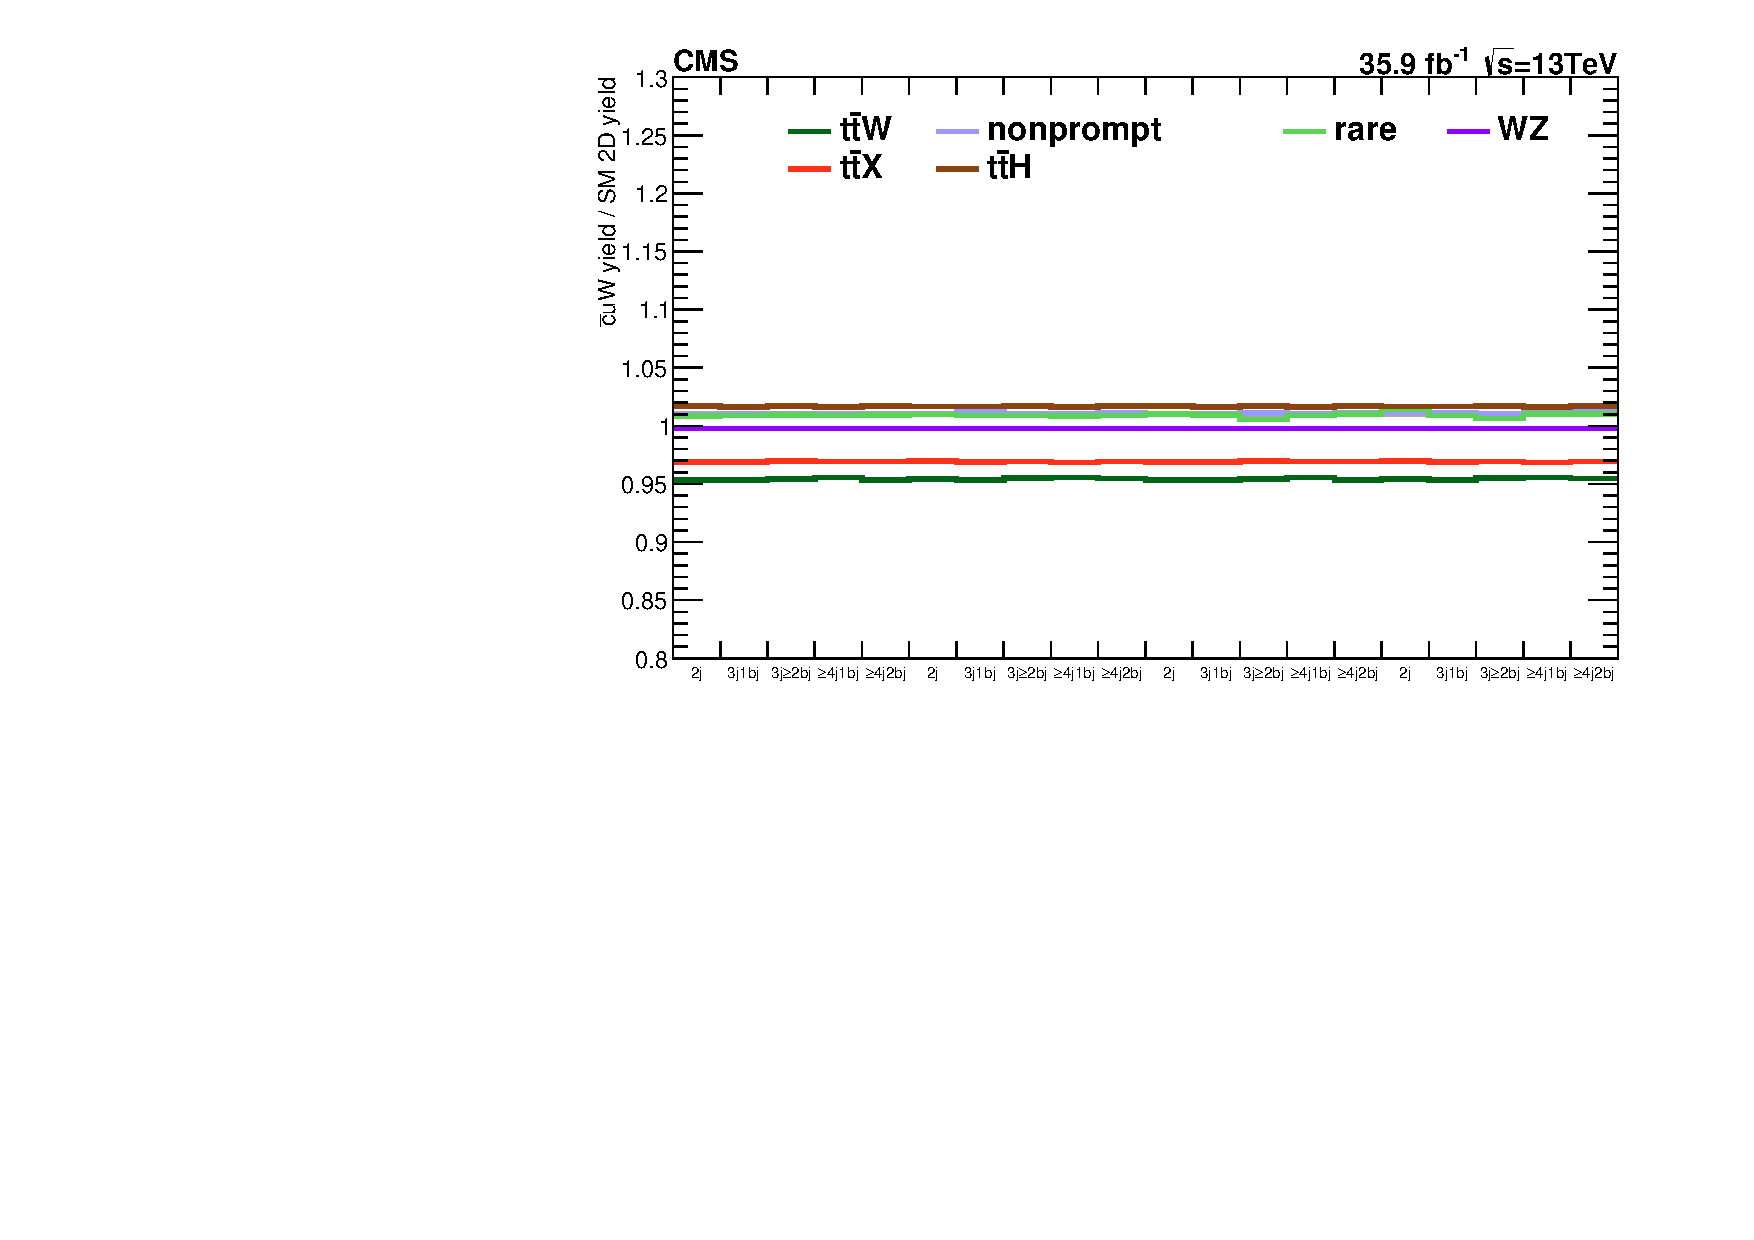
\includegraphics[width=0.5\textwidth]{figures/thirteen-TeV/postfit/ratio_2l_cuW}%
    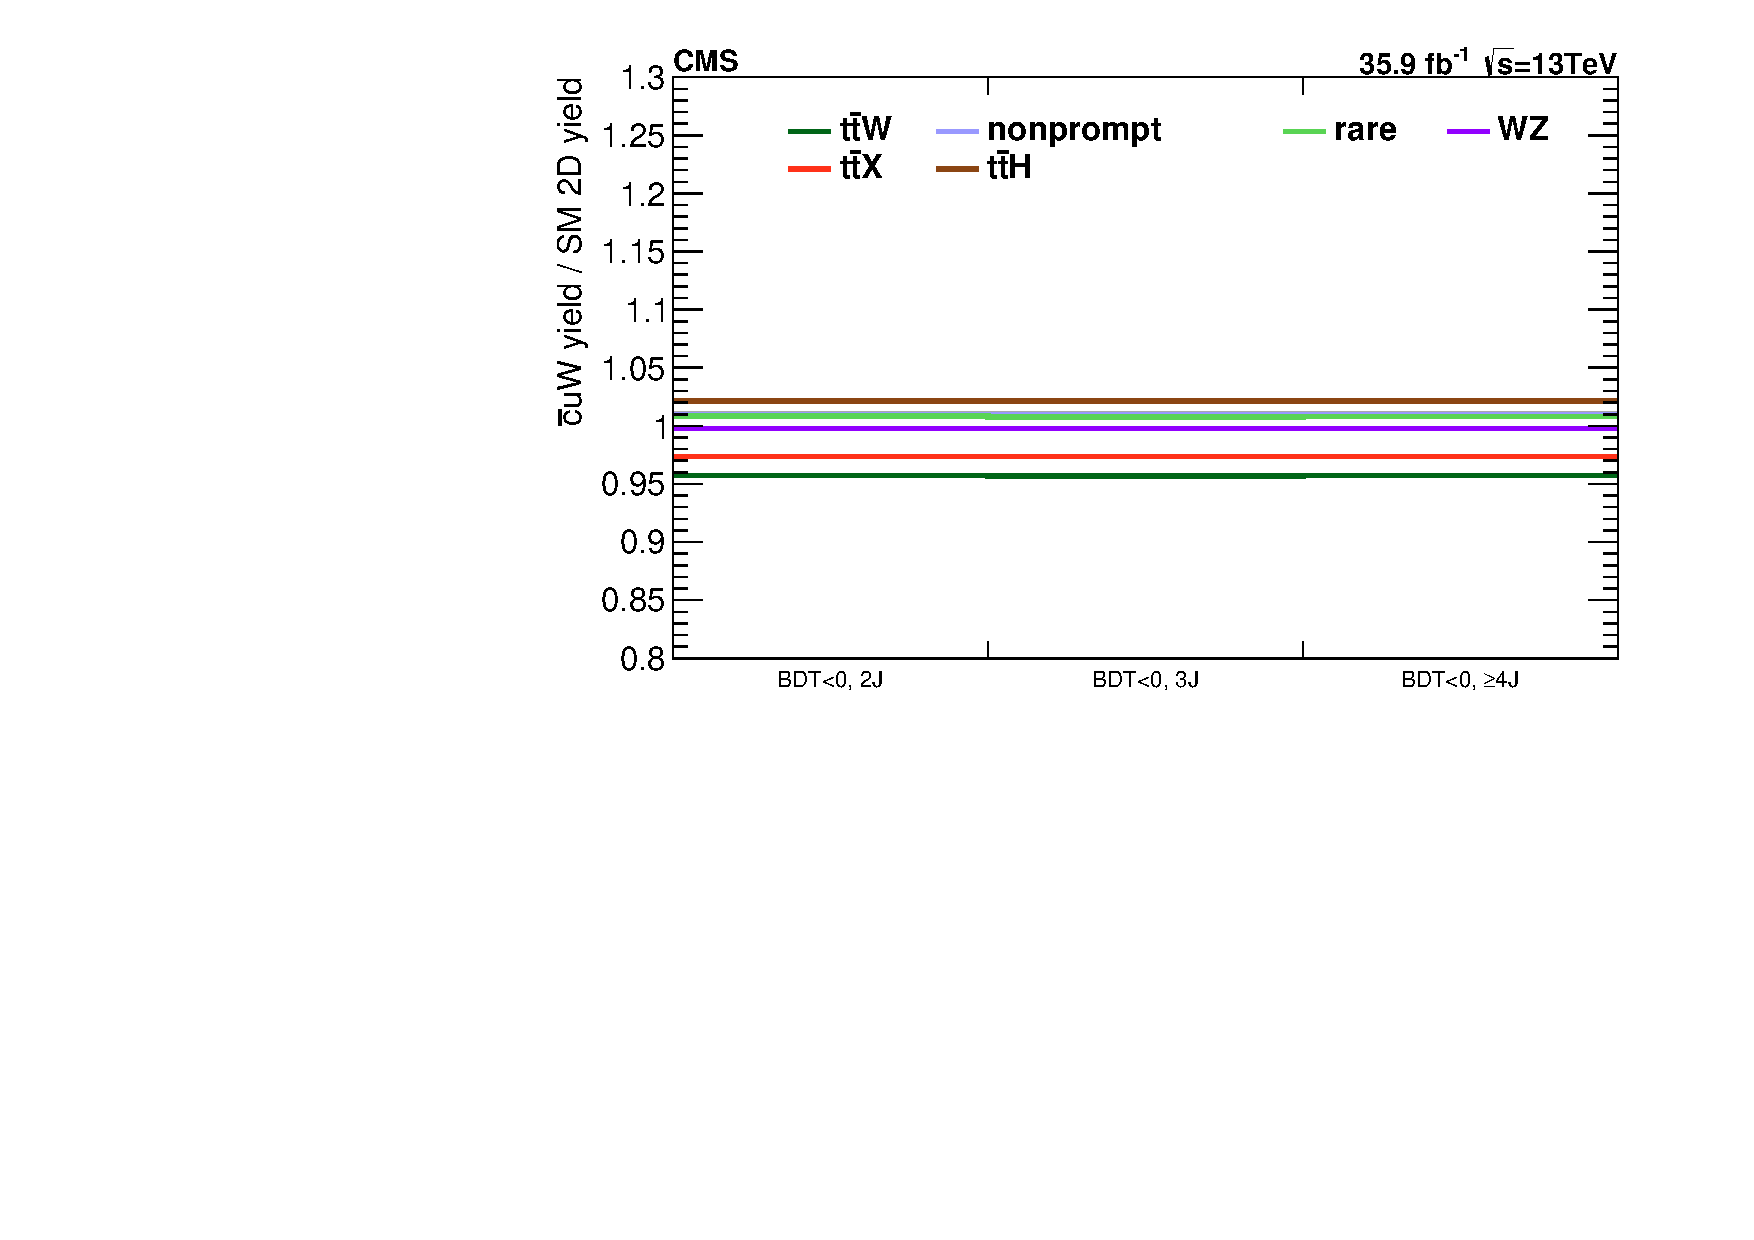
\includegraphics[width=0.5\textwidth]{figures/thirteen-TeV/postfit/ratio_2l-cr_cuW}
    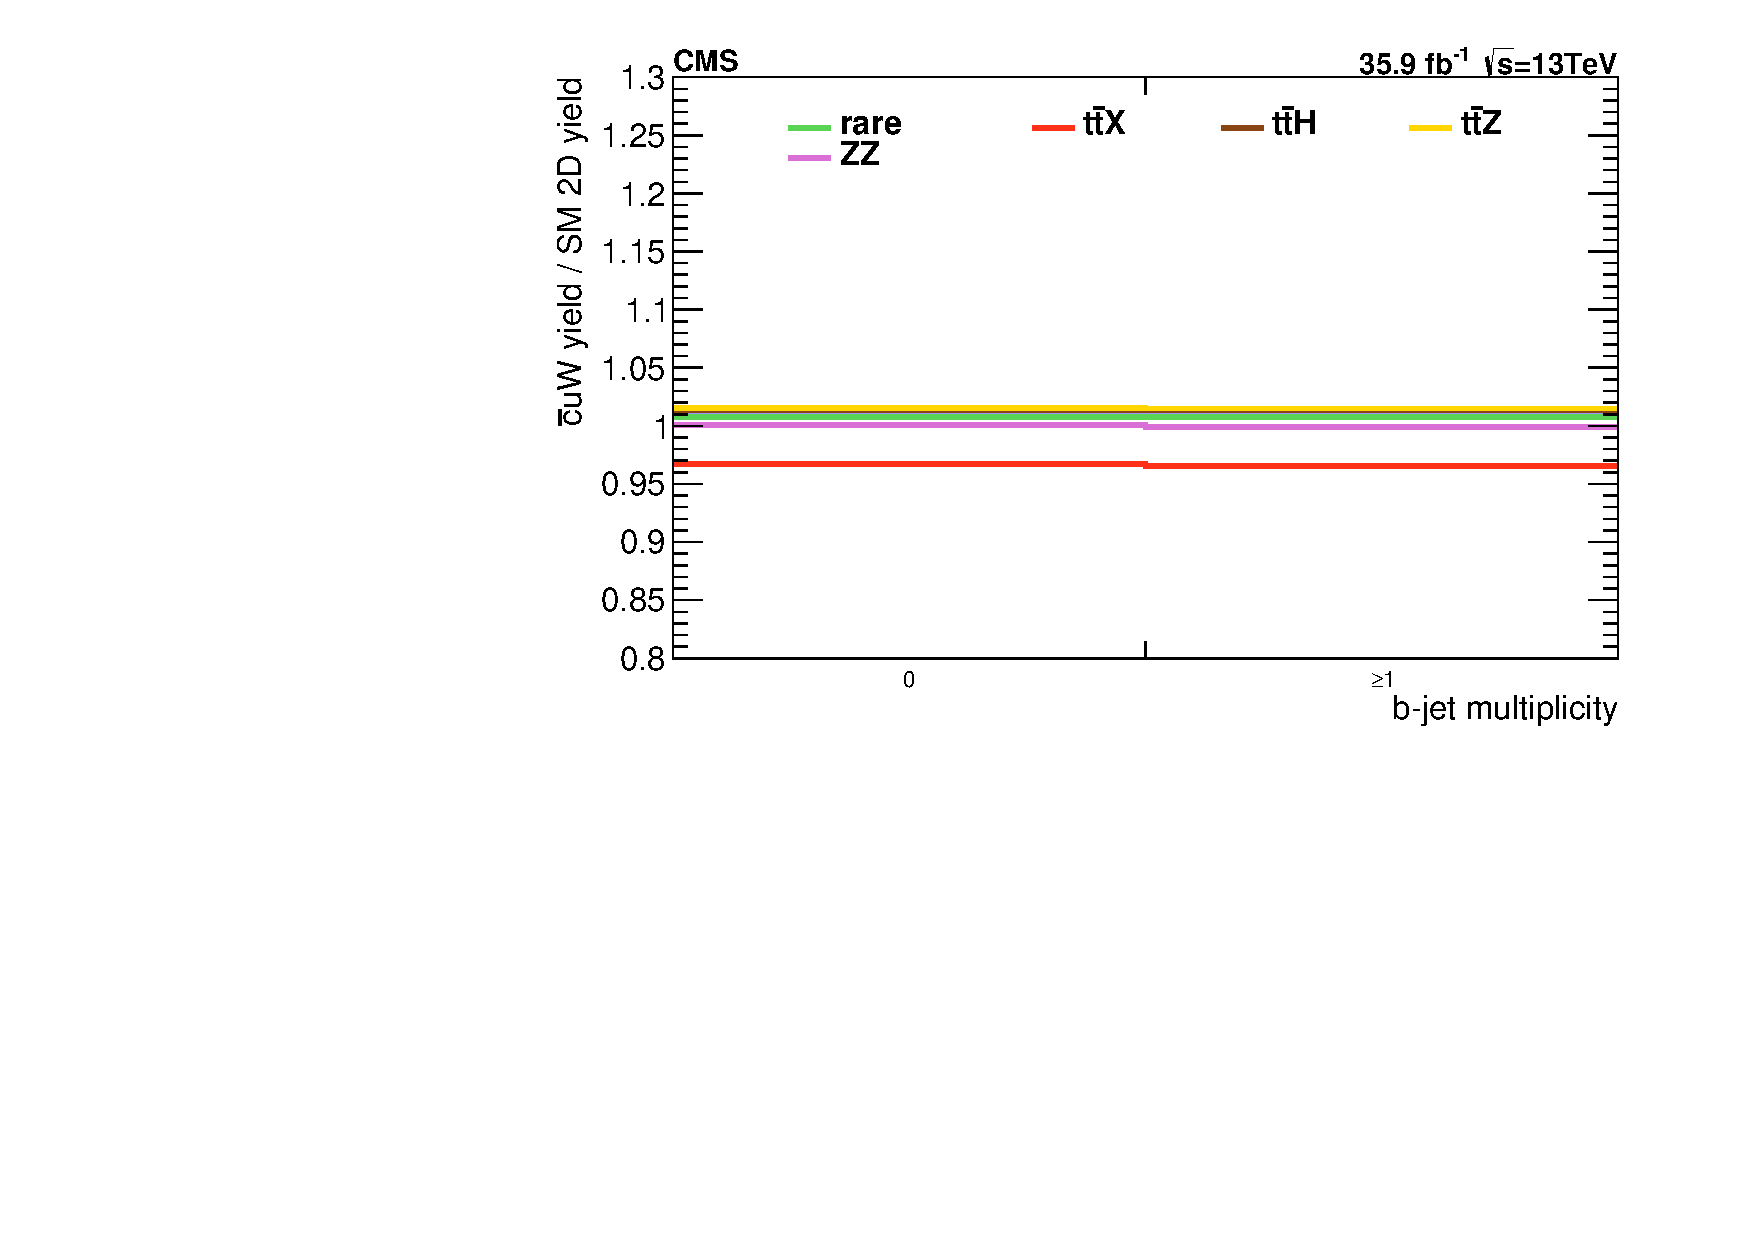
\includegraphics[width=0.5\textwidth]{figures/thirteen-TeV/postfit/ratio_4l_cuW}%
    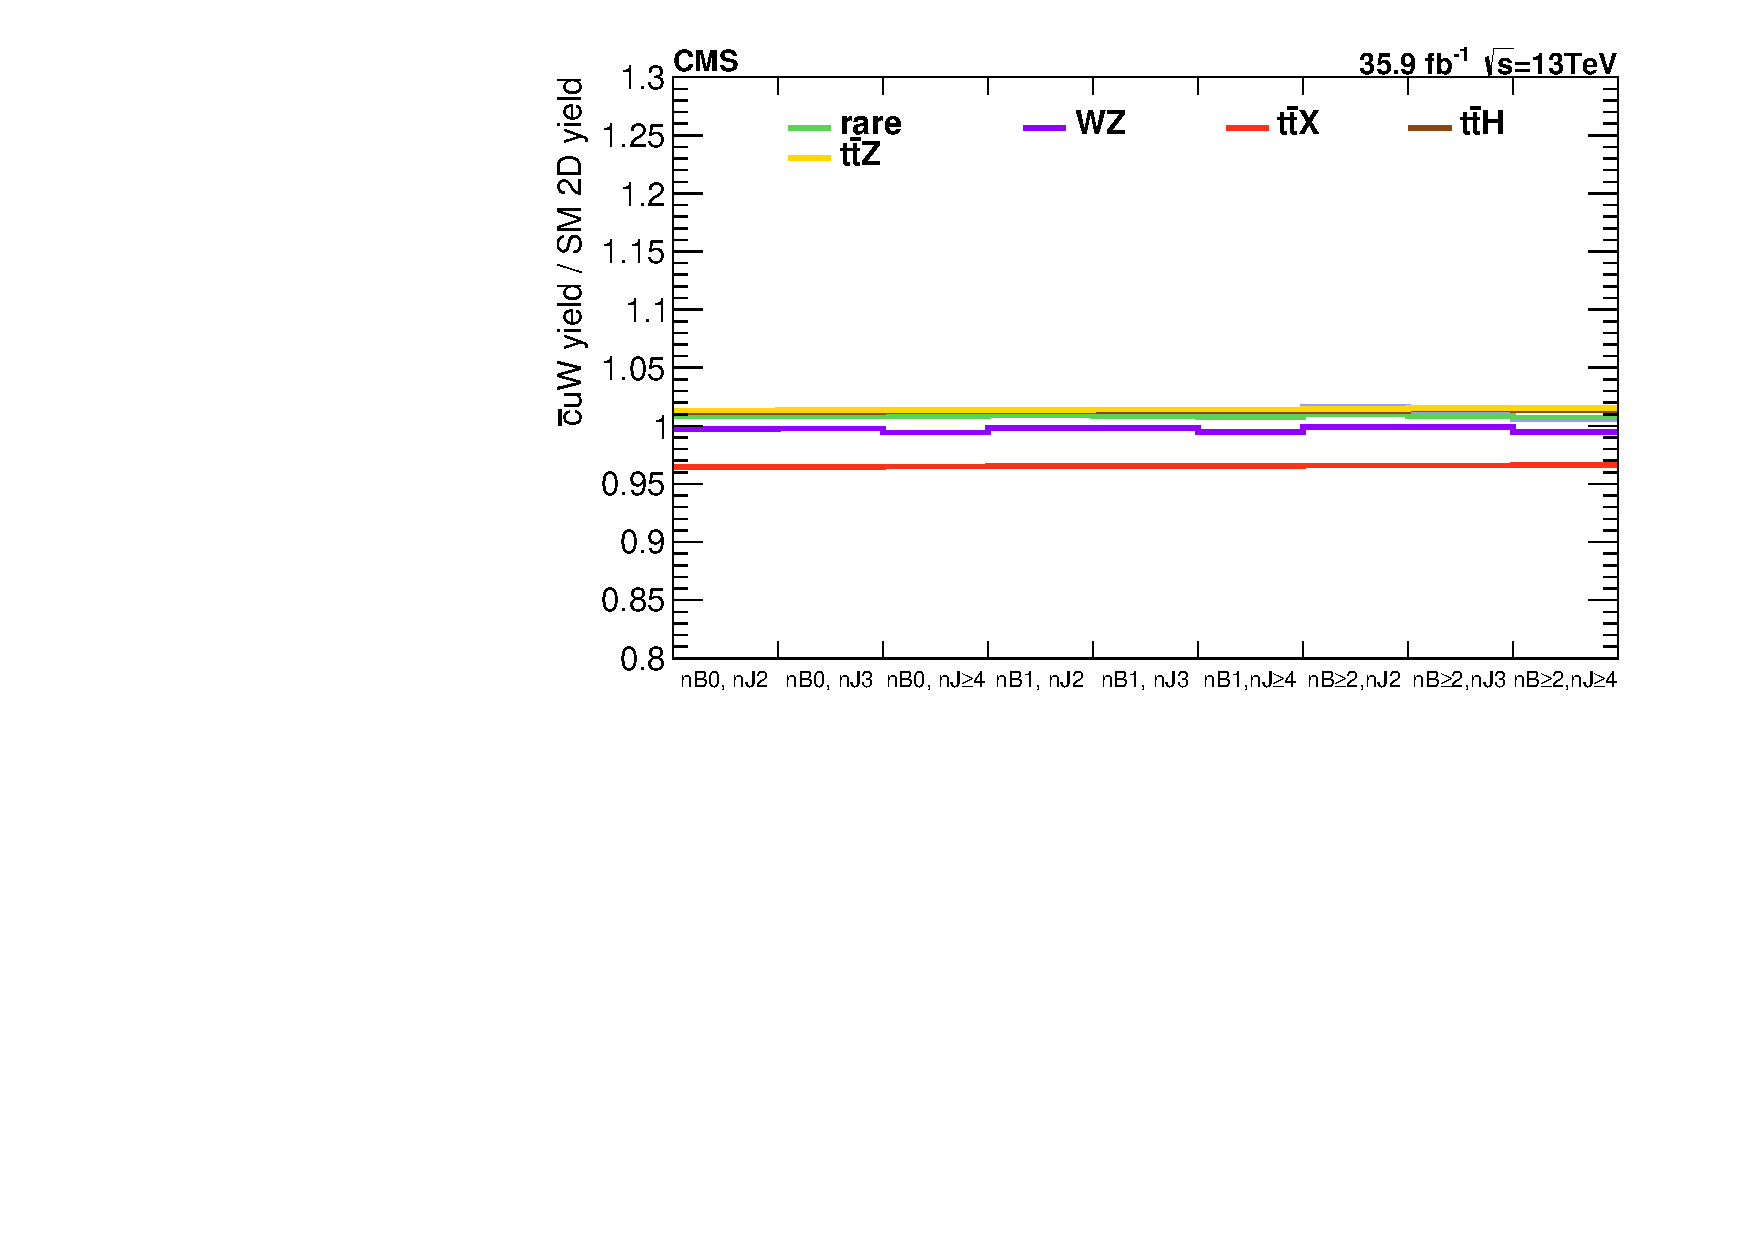
\includegraphics[width=0.5\textwidth]{figures/thirteen-TeV/postfit/ratio_3l_cuW}
    \caption{}
    \label{sfig:ratio-cuW}
  \end{subfigure}
  \caption[Ratio of two and one-dimensional fit yields for \cuG and \cuW (\thirteenTeV)]{Ratio of yields resulting from the fit with two free parameters for $\mu_{\ttW}$ and $\mu_{\ttZ}$ to those from the fit with one free parameter for $c_1$. In~\subref{sfig:ratio-cuG}, panels refer to (clockwise from top left) the SS \ttW signal region with $D > 0$ and control region with $D < 0$, the 3\lep \ttZ channel, and the 4\lep \ttZ channel for \cuG, and similarly in~\subref{sfig:ratio-cuW} for \cuW.}
    \label{fig:ratio-cuG-cuW}
\end{figure}
\begin{figure}
  \begin{subfigure}{\linewidth}
    \centering
      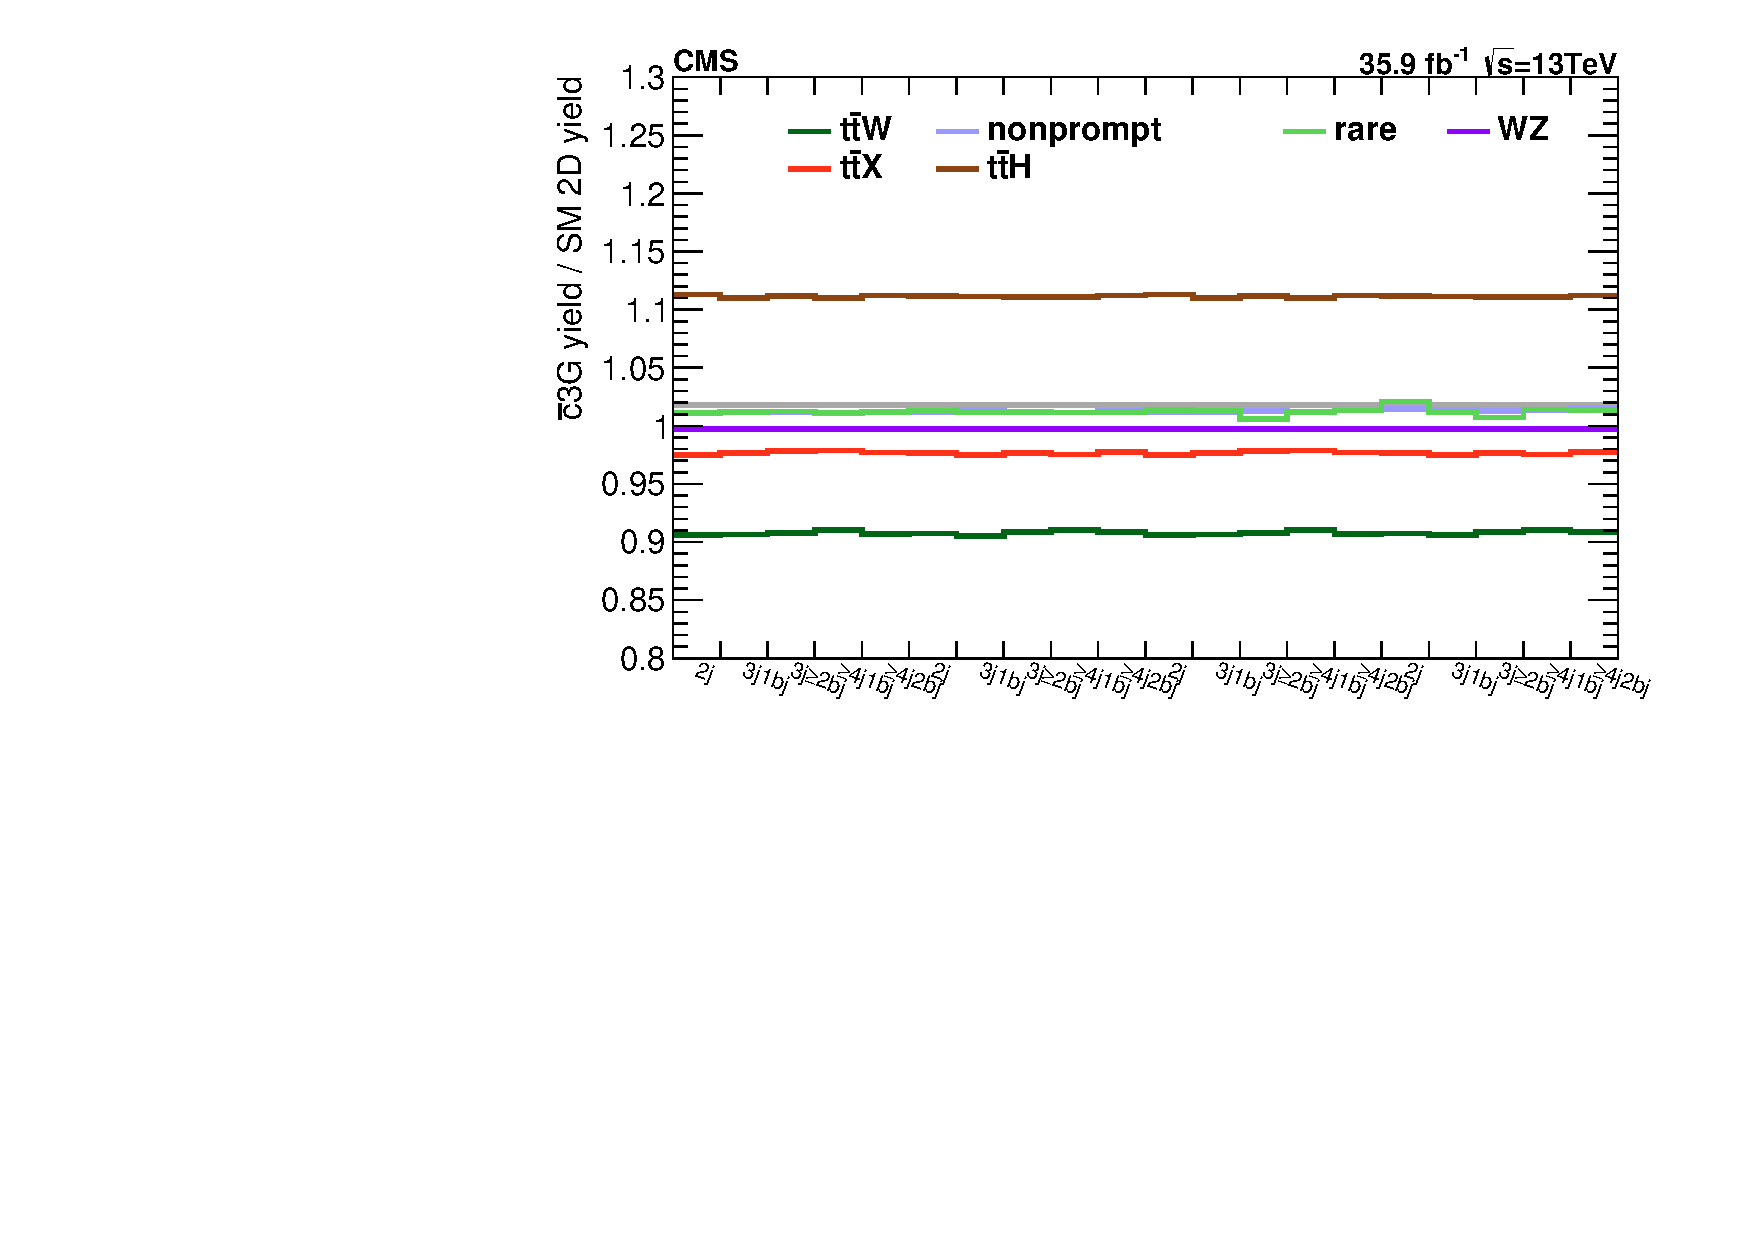
\includegraphics[width=0.5\linewidth]{figures/thirteen-TeV/postfit/ratio_2l_c3G}%
      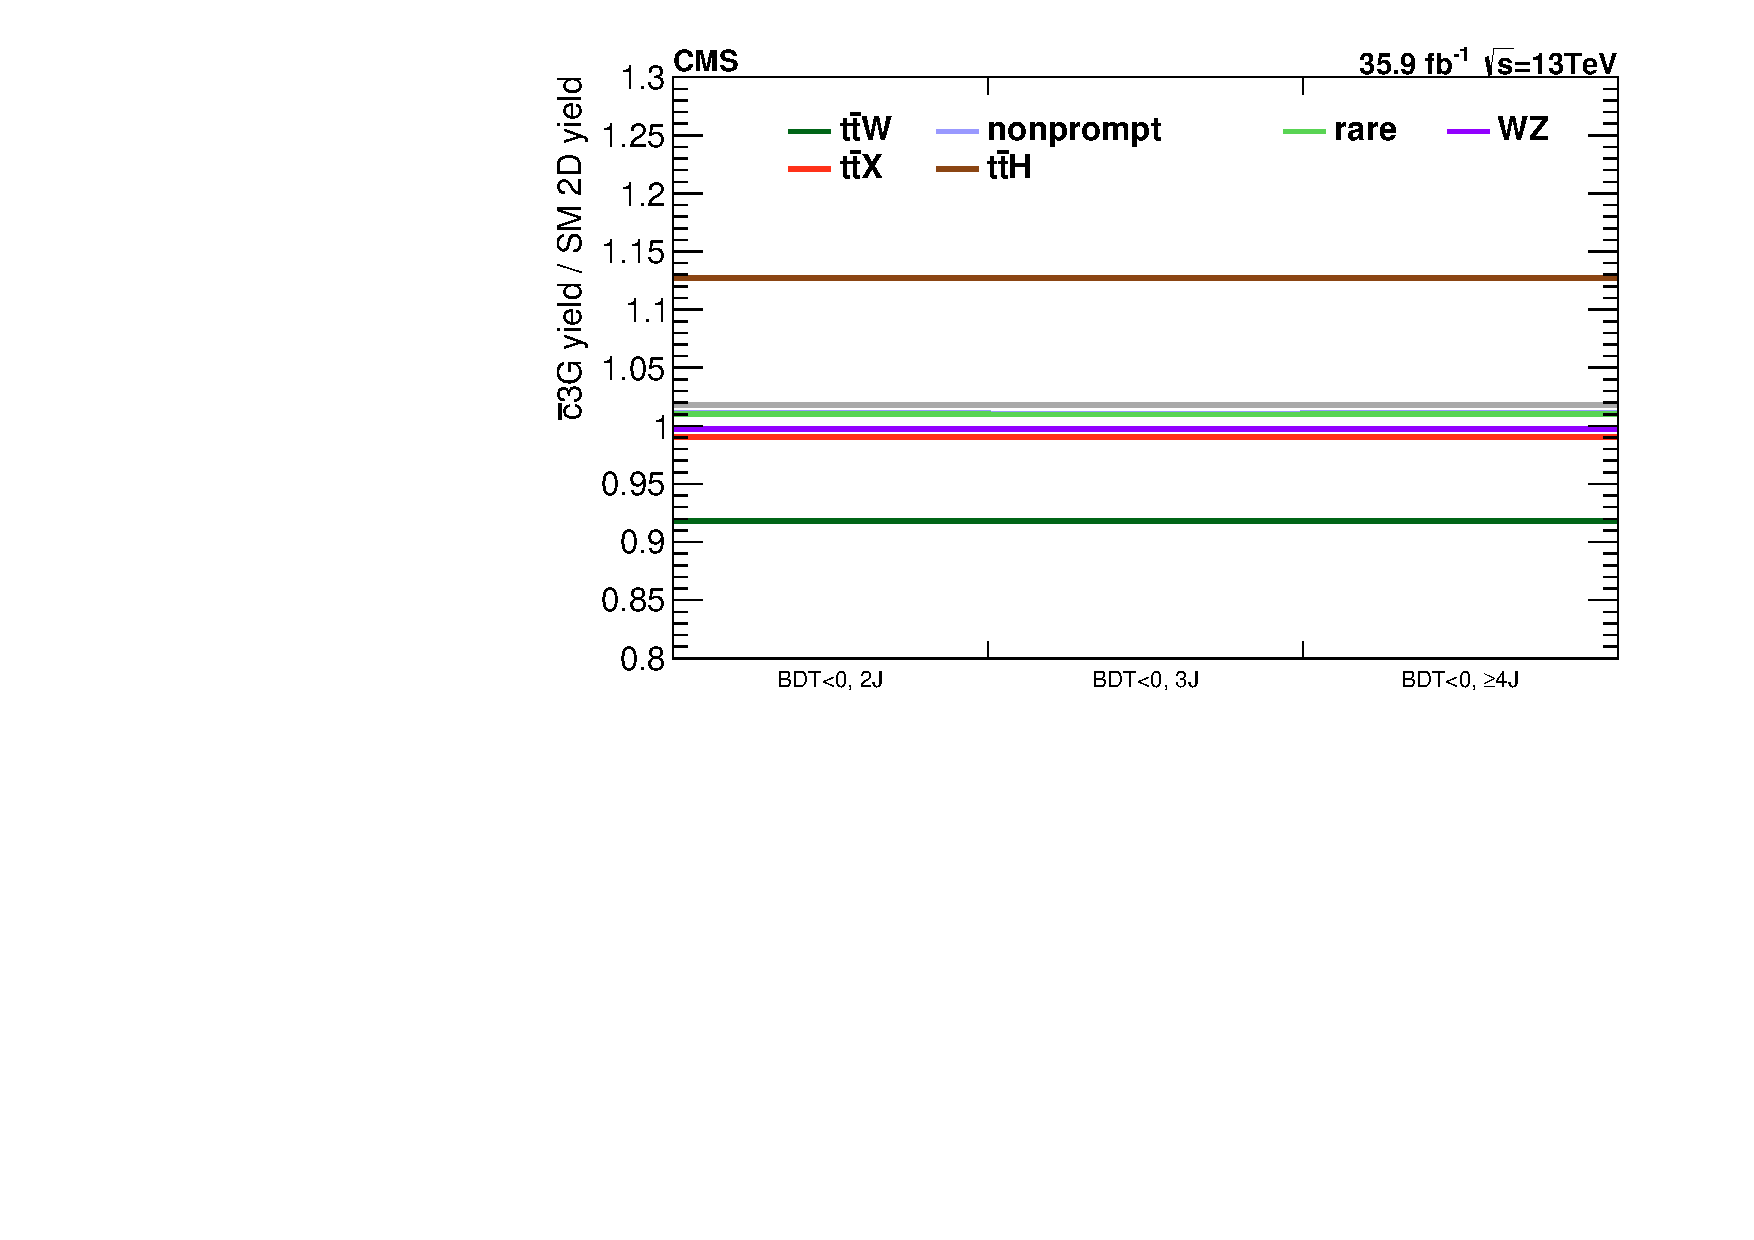
\includegraphics[width=0.5\linewidth]{figures/thirteen-TeV/postfit/ratio_2l-cr_c3G}
      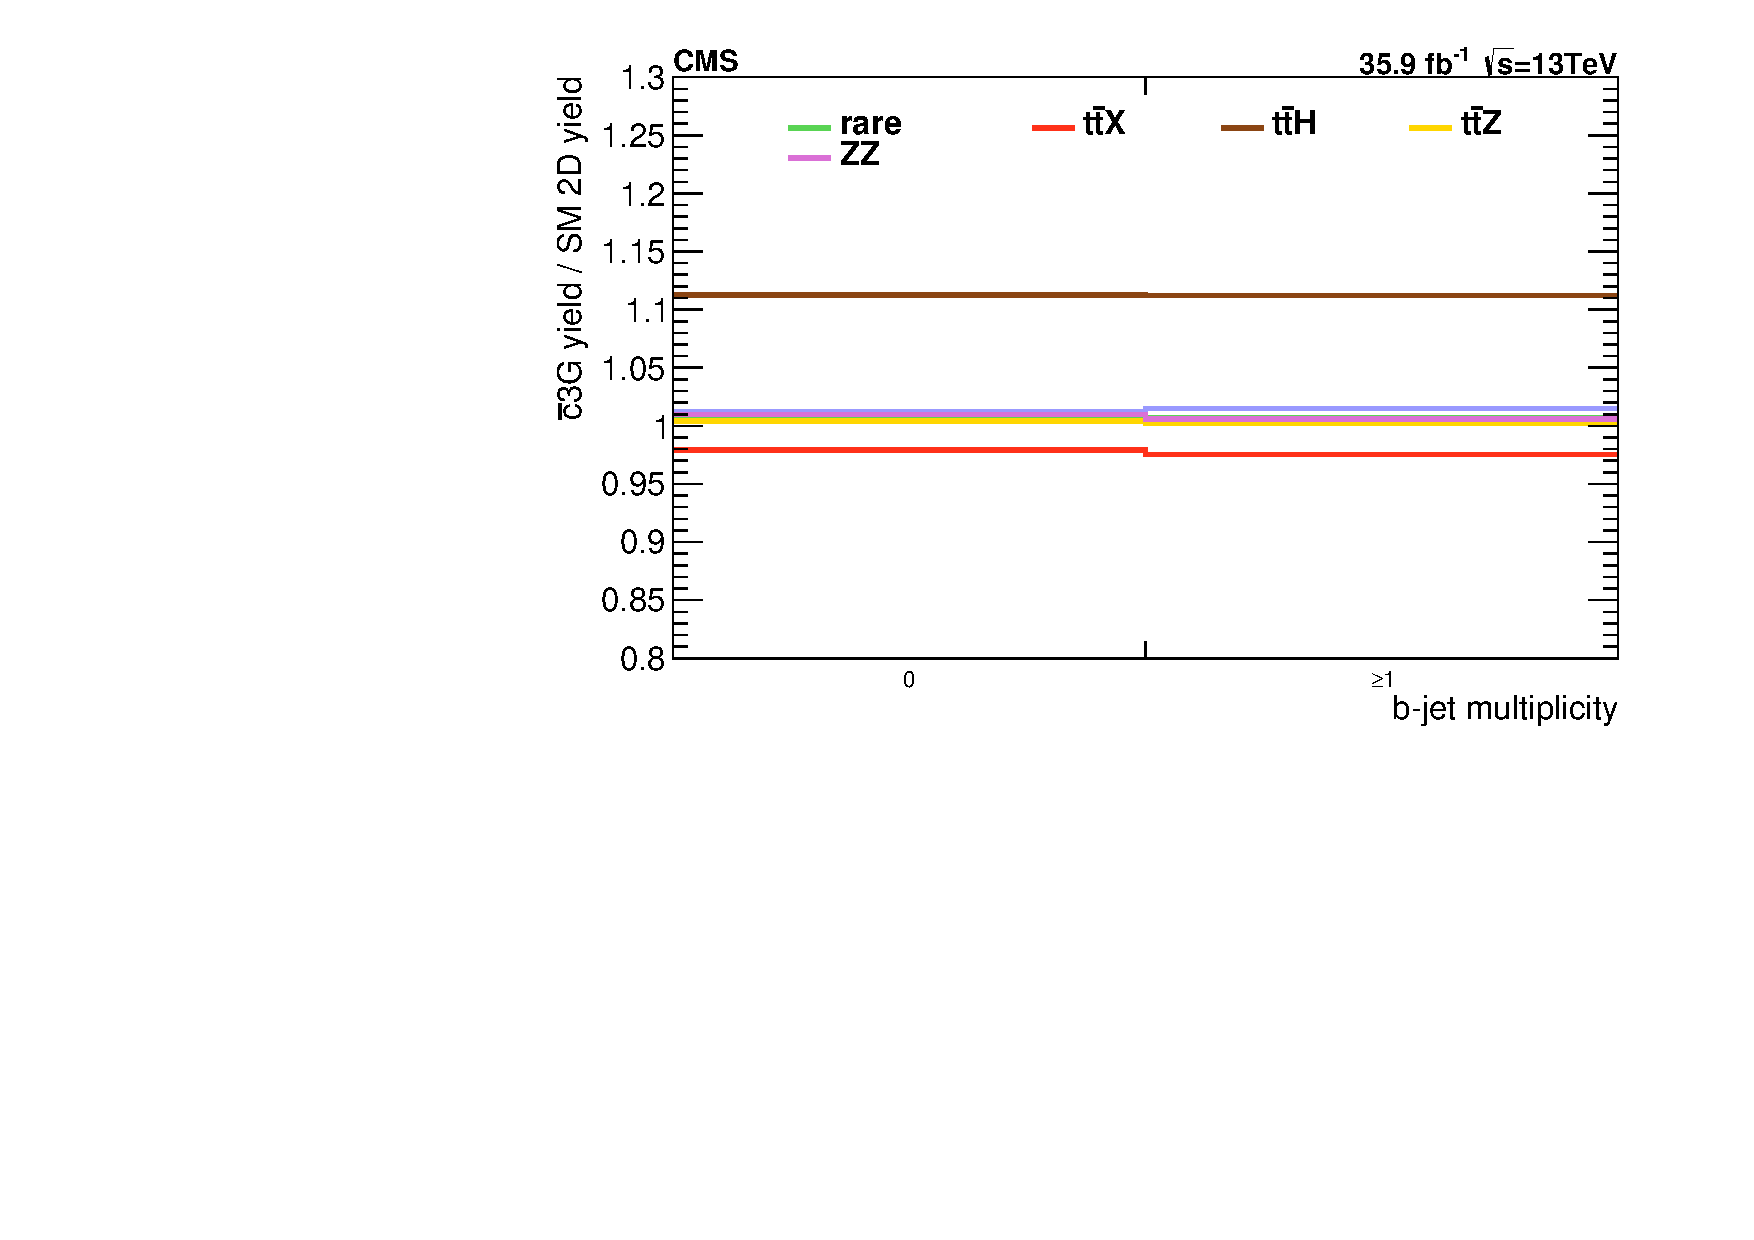
\includegraphics[width=0.5\linewidth]{figures/thirteen-TeV/postfit/ratio_4l_c3G}%
      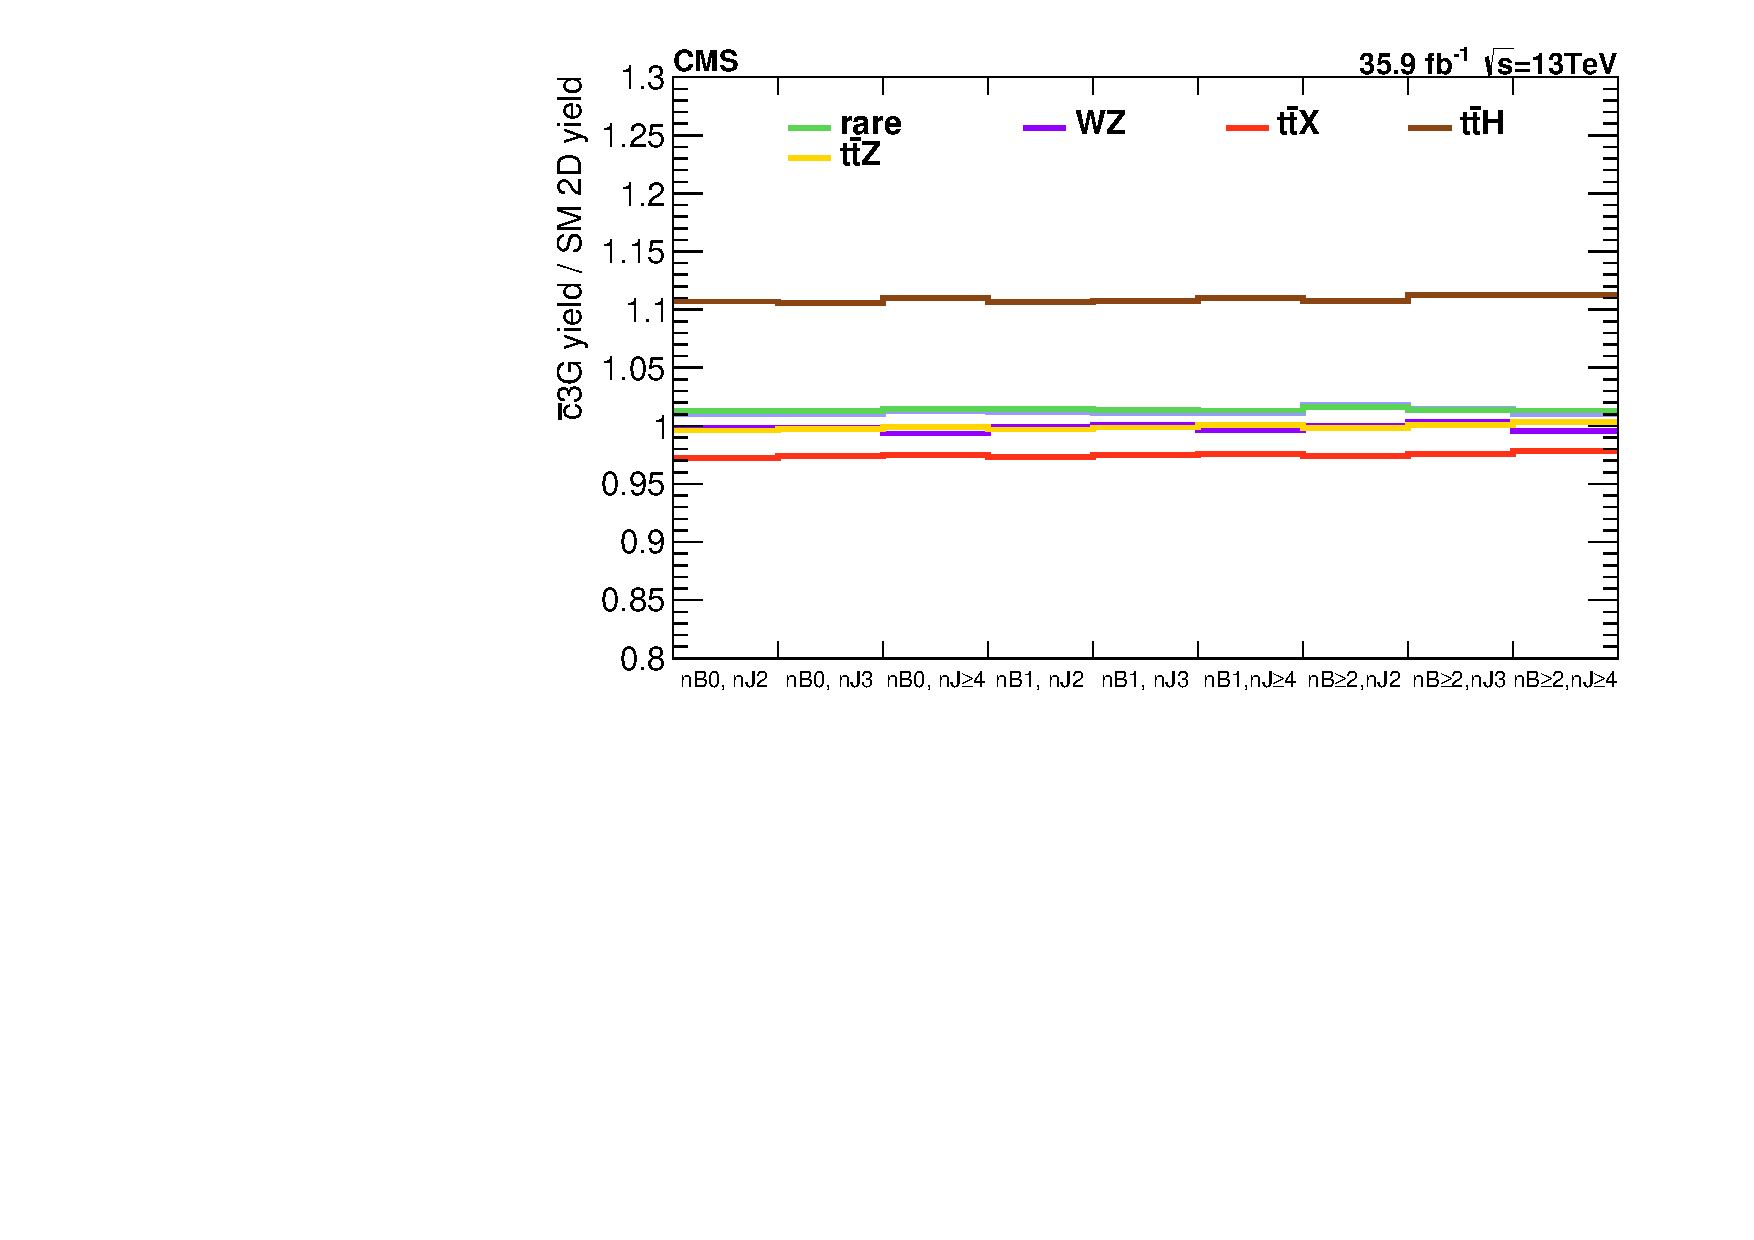
\includegraphics[width=0.5\linewidth]{figures/thirteen-TeV/postfit/ratio_3l_c3G}
    \caption{}
    \label{sfig:ratio-c3G}
  \end{subfigure}
  \begin{subfigure}{\linewidth}
    \centering
    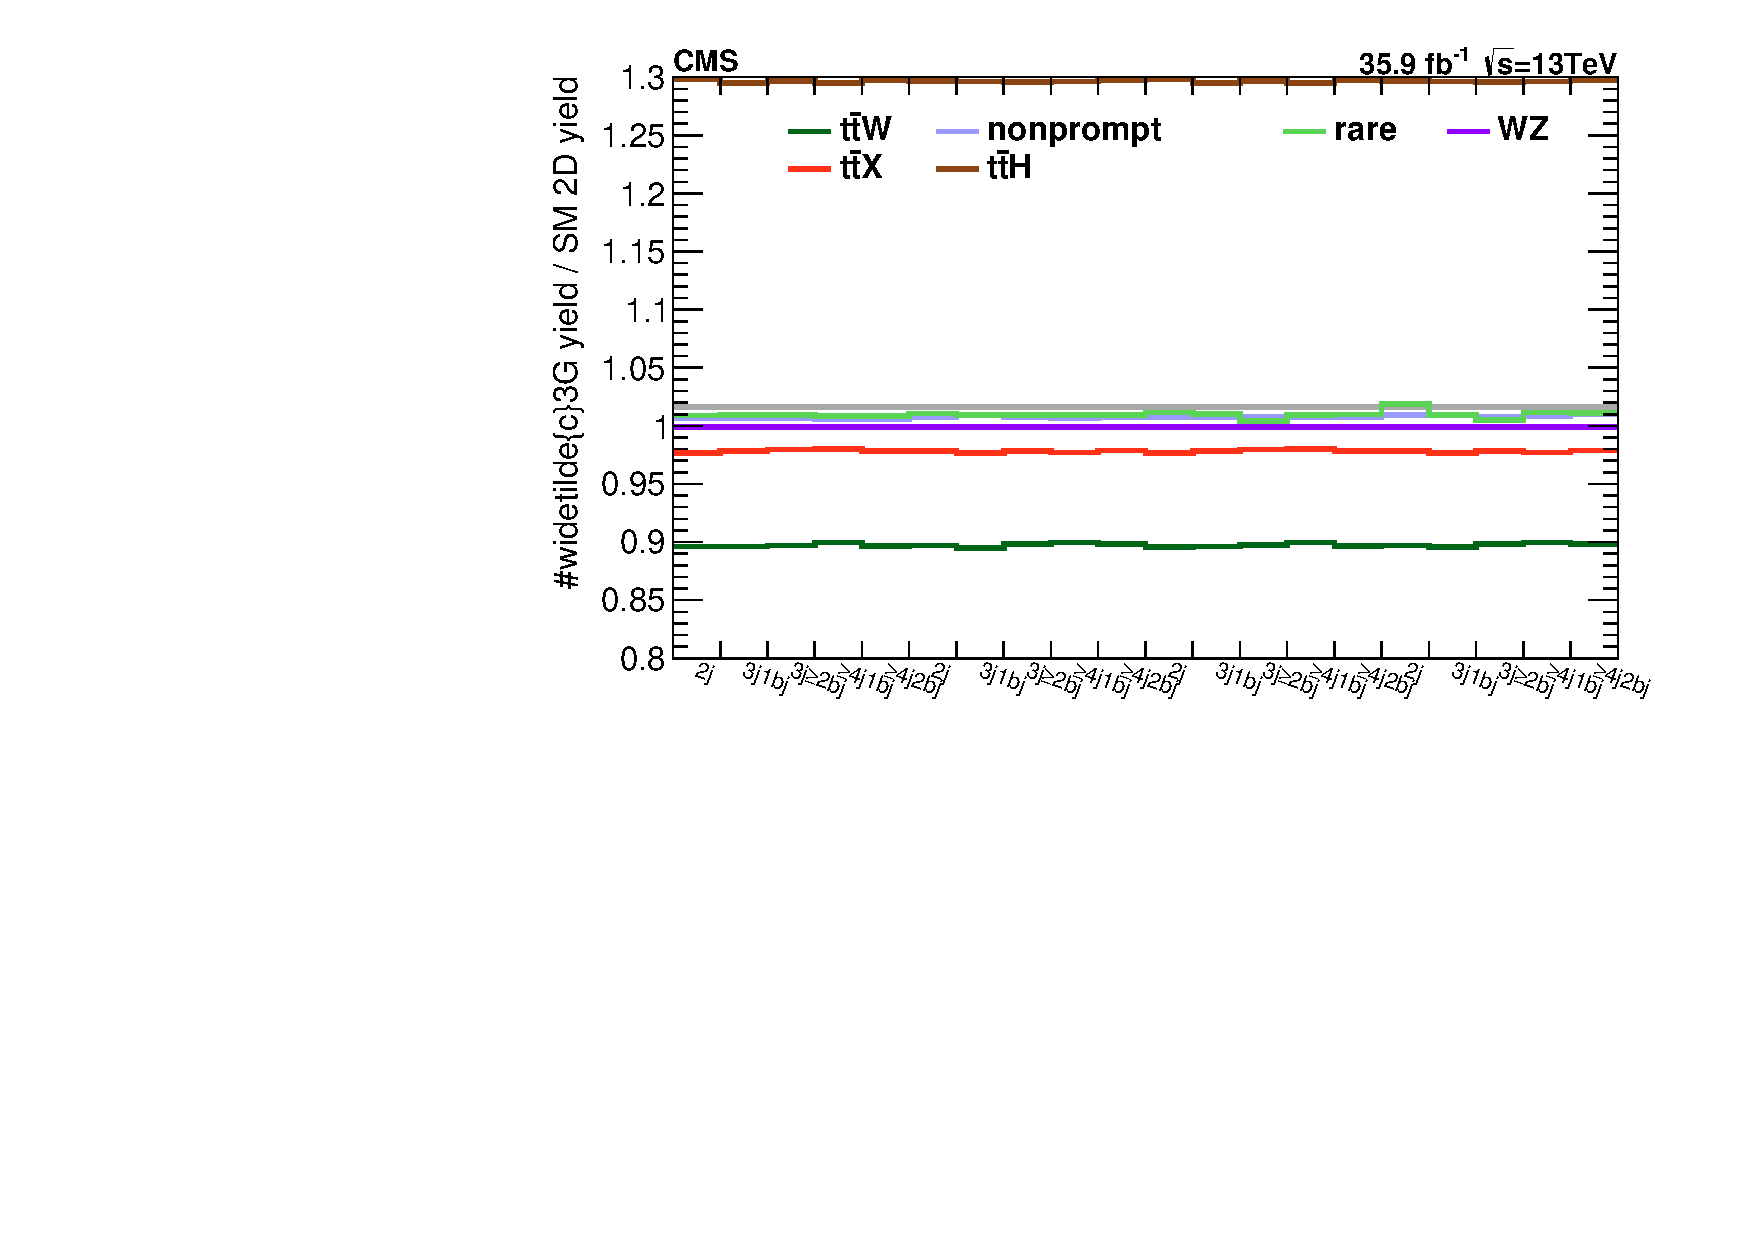
\includegraphics[width=0.5\textwidth]{figures/thirteen-TeV/postfit/ratio_2l_tc3G}%
    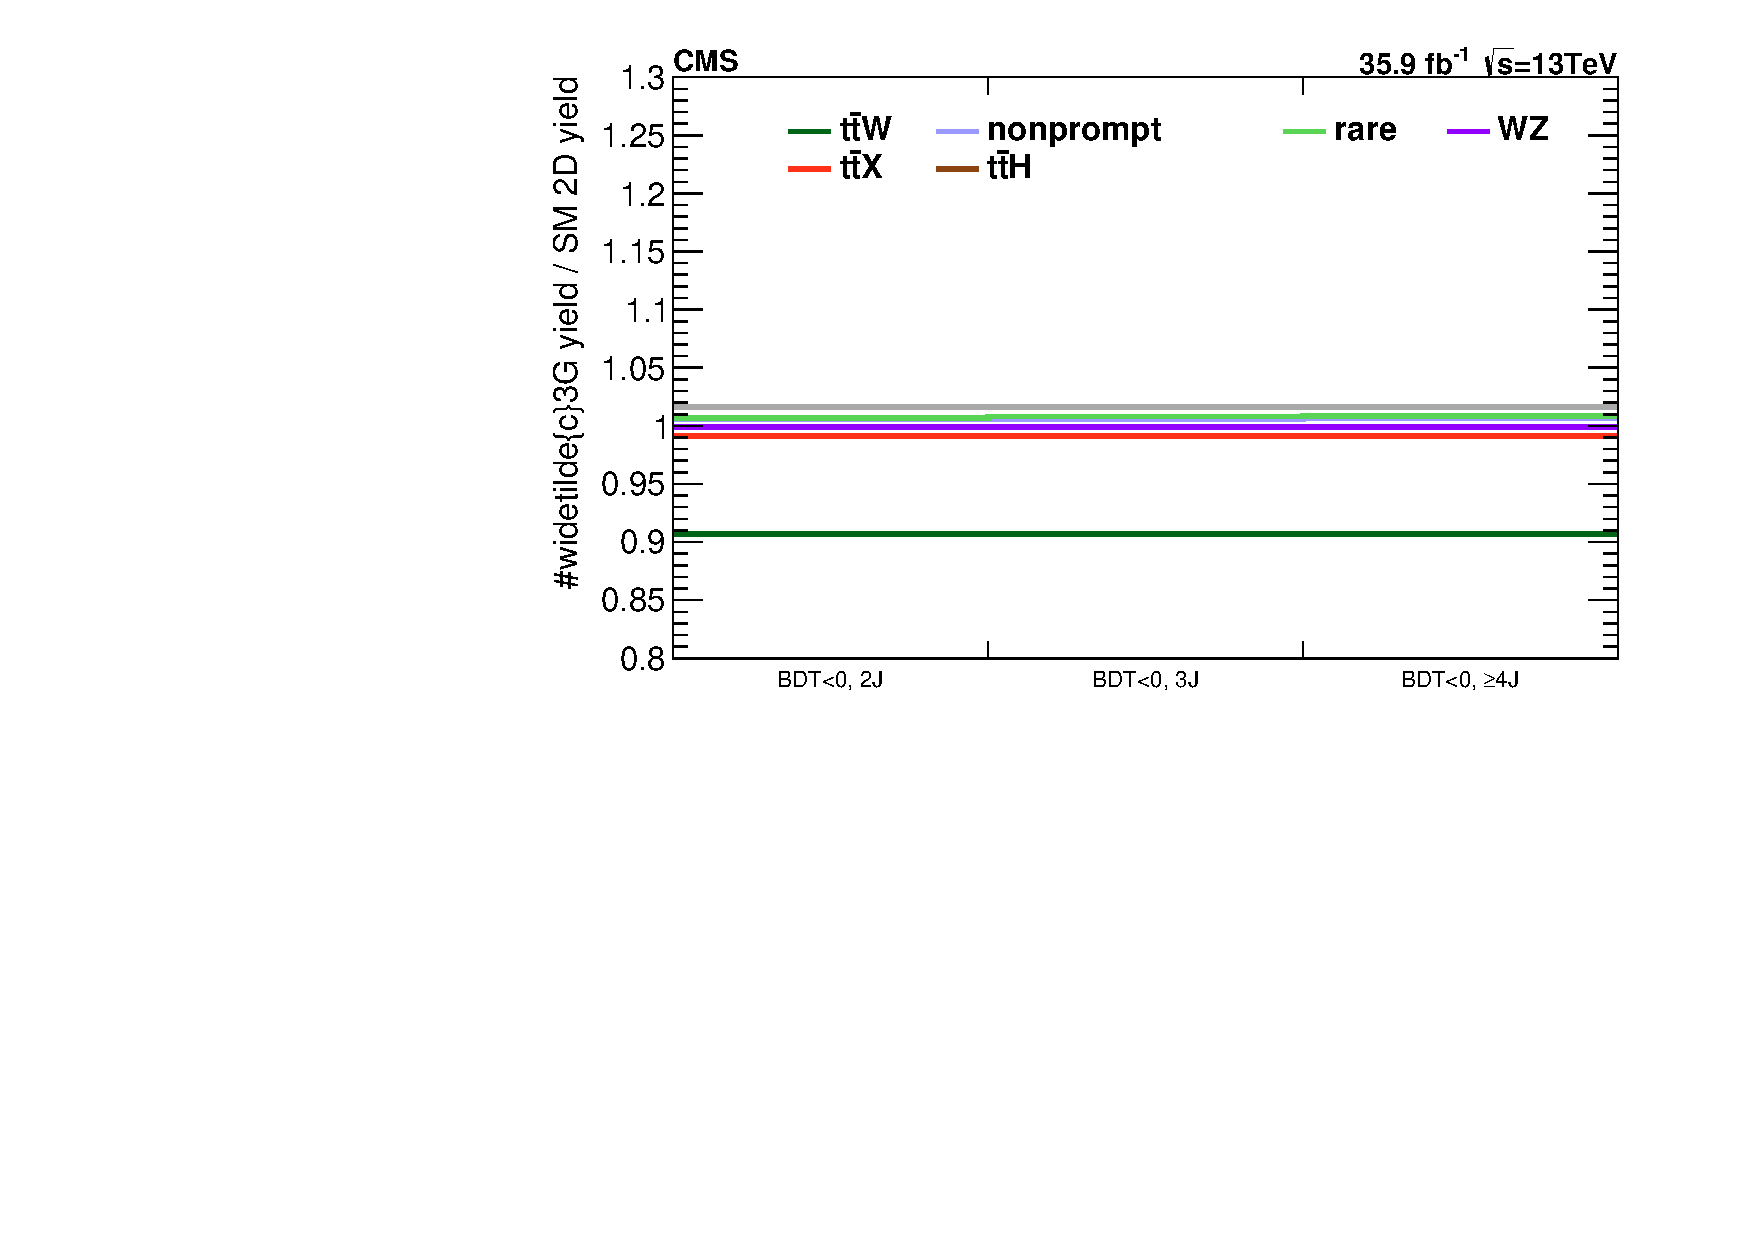
\includegraphics[width=0.5\textwidth]{figures/thirteen-TeV/postfit/ratio_2l-cr_tc3G}
    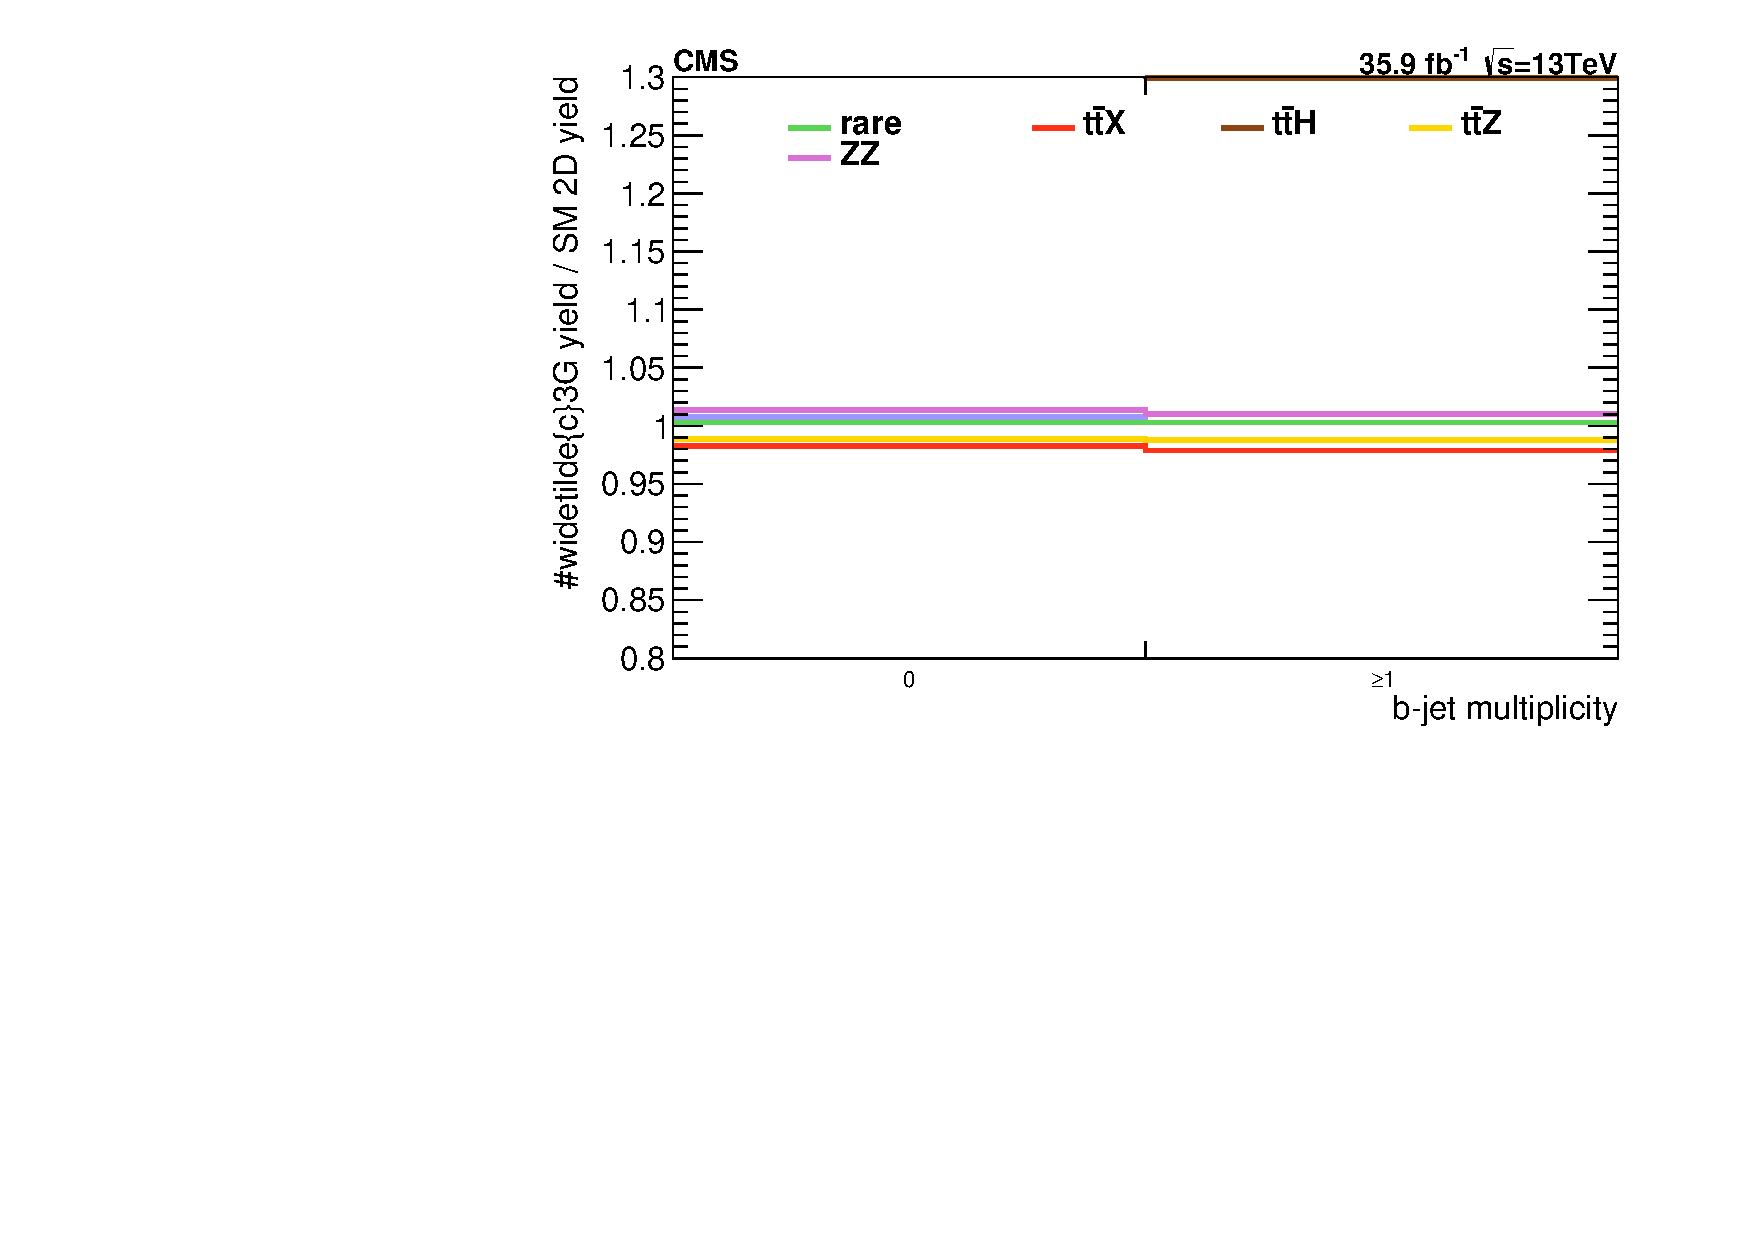
\includegraphics[width=0.5\textwidth]{figures/thirteen-TeV/postfit/ratio_4l_tc3G}%
    \includegraphics[width=0.5\textwidth]{figures/thirteen-TeV/postfit/ratio_3l_tc3G}
    \caption{}
    \label{sfig:ratio-tc3G}
  \end{subfigure}
  \caption[Ratio of two and one-dimensional fit yields for \cthreeG and \cthreeG (\thirteenTeV)]{Ratio of yields resulting from the fit with two free parameters for $\mu_{\ttW}$ and $\mu_{\ttZ}$ to those from the fit with one free parameter for $c_1$. In~\subref{sfig:ratio-c3G}, panels refer to (clockwise from top left) the SS \ttW signal region with $D > 0$ and control region with $D < 0$, the 3\lep \ttZ channel, and the 4\lep \ttZ channel for \cthreeG, and similarly in~\subref{sfig:ratio-tc3G} for \tcthreeG.}
  \label{fig:ratio-c3G-tc3G}
\end{figure}
\begin{figure}
  \begin{subfigure}{\linewidth}
    \centering
      \includegraphics[width=0.5\linewidth]{figures/thirteen-TeV/postfit/ratio_2l_c2G}%
      \includegraphics[width=0.5\linewidth]{figures/thirteen-TeV/postfit/ratio_2l-cr_c2G}
      \includegraphics[width=0.5\linewidth]{figures/thirteen-TeV/postfit/ratio_4l_c2G}%
      \includegraphics[width=0.5\linewidth]{figures/thirteen-TeV/postfit/ratio_3l_c2G}
    \caption{}
    \label{sfig:ratio-c2G}
  \end{subfigure}
  \begin{subfigure}{\linewidth}
    \centering
    \includegraphics[width=0.5\textwidth]{figures/thirteen-TeV/postfit/ratio_2l_cuB}%
    \includegraphics[width=0.5\textwidth]{figures/thirteen-TeV/postfit/ratio_2l-cr_cuB}
    \includegraphics[width=0.5\textwidth]{figures/thirteen-TeV/postfit/ratio_4l_cuB}%
    \includegraphics[width=0.5\textwidth]{figures/thirteen-TeV/postfit/ratio_3l_cuB}
    \caption{}
    \label{sfig:ratio-cuB}
  \end{subfigure}
  \caption[Ratio of two and one-dimensional fit yields for \ctwoG and \cuB (\thirteenTeV)]{Ratio of yields resulting from the fit with two free parameters for $\mu_{\ttW}$ and $\mu_{\ttZ}$ to those from the fit with one free parameter for $c_1$. In~\subref{sfig:ratio-c2G}, panels refer to (clockwise from top left) the SS \ttW signal region with $D > 0$ and control region with $D < 0$, the 3\lep \ttZ channel, and the 4\lep \ttZ channel for \ctwoG, and similarly in~\subref{sfig:ratio-cuB} for \cuB.}
  \label{fig:ratio-c2G-cuB}
\end{figure}
\begin{figure}
  \begin{subfigure}{\linewidth}
    \centering
      \includegraphics[width=0.5\textwidth]{figures/thirteen-TeV/postfit/ratio_2l_cH}%
      \includegraphics[width=0.5\textwidth]{figures/thirteen-TeV/postfit/ratio_2l-cr_cH}
      \includegraphics[width=0.5\textwidth]{figures/thirteen-TeV/postfit/ratio_4l_cH}%
      \includegraphics[width=0.5\textwidth]{figures/thirteen-TeV/postfit/ratio_3l_cH}
    \caption{}
    \label{sfig:ratio-cH}
  \end{subfigure}
  \begin{subfigure}{\linewidth}
    \centering
    \includegraphics[width=0.5\textwidth]{figures/thirteen-TeV/postfit/ratio_2l_cHu}%
    \includegraphics[width=0.5\textwidth]{figures/thirteen-TeV/postfit/ratio_2l-cr_cHu}
    \includegraphics[width=0.5\textwidth]{figures/thirteen-TeV/postfit/ratio_3l_cHu}%
    \includegraphics[width=0.5\textwidth]{figures/thirteen-TeV/postfit/ratio_4l_cHu}
    \caption{}
    \label{sfig:ratio-cHu}
  \end{subfigure}
  \caption[Ratio of two and one-dimensional fit yields for \cH and \cHu (\thirteenTeV)]{Ratio of yields resulting from the fit with two free parameters for $\mu_{\ttW}$ and $\mu_{\ttZ}$ to those from the fit with one free parameter for $c_1$. In~\subref{sfig:ratio-cH}, panels refer to (clockwise from top left) the SS \ttW signal region with $D > 0$ and control region with $D < 0$, the 3\lep \ttZ channel, and the 4\lep \ttZ channel for \cH, and similarly in~\subref{sfig:ratio-cHu} for \cHu.}
  \label{fig:ratio-cH-cHu}
\end{figure}

\subsection{Preliminary simultaneous constraints}
\label{ssec:simultaneous-eft}
The results of the previous sections, obtained by considering the effects of
each dimension-six operator with the others fixed to zero, are an important
first step. They rely on the assumption that NP processes only enhance certain
Wilson coefficients; however, this case is special. Additional work is needed to
remove this assumption and generalize the results by performing a simultaneous
fit to all Wilson coefficients, which would provide a more meaningful
description of the underlying physics. Fortunately, adapting \cref{eq:np-xsec},
used in the previous sections to parameterize the scaling due one operator at a
time, for two operators is straightforward:
\begin{align}
  \sigma(c_1, c_2) &\propto \lvert\mathcal{M}_\text{SM} + c_1\mathcal{M}_1 + c_2\mathcal{M}_2\rvert^2 \\
  &\propto
  \underbrace{s_0}_{\text{constant}} +
  \underbrace{s_1 c_1 + s_2 c_2}_{\text{linear}} +
  \underbrace{s_3 c_1^2 + s_4 c_2^2}_{\text{quadratic}} +
  \underbrace{s_5 c_1 c_2}_{\text{mixed}}.
  \label{eq:2d}
\end{align}
And for three operators:
\begin{align}
  \sigma(c_1, c_2, c_3) &\propto \lvert\mathcal{M}_\text{SM} + c_1\mathcal{M}_1 + c_2\mathcal{M}_2 + c_3\mathcal{M}_3\rvert^2 \\
                        &\propto \underbrace{s_0}_{\text{constant}} +
  \underbrace{s_1 c_1 + s_2 c_2 +s_3 c_3}_{\text{linear}} +
  \underbrace{s_4 c_1^2 + s_5 c_2^2 + s_6 c_3^2}_{\text{quadratic}} +
  \underbrace{s_7 c_1 c_2 + s_8 c_1 c_3 + s_9 c_2 c_3}_{\text{mixed}}.
\end{align}
where the structure constants have been re-numbered in order for clarity. There
are only constant, linear, and quadratic terms. For two operators, we can solve
for the six structure constants by evaluating the cross section at six points
(sets of $c_1$ and $c_2$ values); for three operators, we need 10 sets of $c_1$,
$c_2$, and $c_3$ values. In general, if there are $d$ operators under
consideration, there will be $N_s$ structure constants, where
\begin{equation}
  N_s = 1 + 2d + \frac{d}{2}(d - 1).
  \label{eq:nd}
\end{equation}
We need to evaluate the cross section at $N_s$ sets of Wilson coefficient values
to completely specify the system of equations. There is no a priori limit on the
number of operators for which their effects can be parameterized with this
procedure; more operators simply correspond to larger $N_s$. Restricting
ourselves to $d=2$ as an example, and dividing by $\sigma_\text{SM}$ to obtain
the signal scaling function, the system of equations corresponding
to~\cref{eq:2d} can be written as $AX = B$:
\[
  \begin{bmatrix}
    1 & c_{11} & c_{12} & c_{11}^2 & c_{12}^2 & c_{11}c_{12} \\
    1 & c_{21} & c_{22} & c_{21}^2 & c_{22}^2 & c_{21}c_{22} \\
    1 & c_{31} & c_{32} & c_{31}^2 & c_{32}^2 & c_{31}c_{32} \\
    1 & c_{41} & c_{42} & c_{41}^2 & c_{42}^2 & c_{41}c_{42} \\
    1 & c_{51} & c_{52} & c_{51}^2 & c_{52}^2 & c_{51}c_{52} \\
    1 & c_{61} & c_{62} & c_{61}^2 & c_{62}^2 & c_{61}c_{62} \\
  \end{bmatrix}
  \begin{bmatrix}
    s_0 \\
    s_1 \\
    s_2 \\
    s_3 \\
    s_4 \\
    s_5 \\
  \end{bmatrix}
   =
  \begin{bmatrix}
    \mu(c_{11}, c_{12}) \\
    \mu(c_{21}, c_{22}) \\
    \mu(c_{31}, c_{32}) \\
    \mu(c_{41}, c_{42}) \\
    \mu(c_{51}, c_{52}) \\
    \mu(c_{61}, c_{62}) \\
  \end{bmatrix},
\]
where we sample six $c_1$, $c_2$ points and evaluate $\mu(c_1, c_2)$; $c_{11}$
and $c_{12}$ correspond to the first point, $c_{21}$ and $c_{22}$ correspond to
the second point, and so forth. In practice, because the \madgraph calculation
has finite precision, solving the system of equations exactly is usually not
possible. Therefore, we use an overdetermined least-squares fit to $N_d > N_s$
points, where we solve $AX = B$ to determine $X$ by minimizing $||B - AX||^2$.
We choose randomly distributed points in the range of coefficient values
corresponding to $\mu(c_1) < 10$ for the 1D case. An example implementation in
Python is presented in~\cref{fig:code}.
\begin{figure}
  % TODO put realistic/actual values below for B; more than six points to show overdetermination
  \small
  \definecolor{bg}{rgb}{0.95,0.95,0.95}
  \begin{minted}[bgcolor=bg]{python}
import numpy as np
import itertools

# sampled coefficient values (two coefficients, six points)
points = np.array([
    [0.78,  0.41],
    [0.95,  0.46],
    [0.98,  0.21],
    [0.83,  0.85],
    [0.76,  0.03],
    [0.46,  0.29]
])

# NP scaling per point (from MadGraph calculation)
B = np.array([4.45, 5.55, 4.53, 7.02, 2.96, 2.74])

rows, dim = points.shape
pairs = list(itertools.combinations(range(0, dim), 2))
left = [x0 for x0, x1 in pairs]
right = [x1 for x0, x1 in pairs]

constant = np.array([[1.0]] * rows)
linear = points
quad = points * points
mixed = points[:, left] * points[:, right]

A = np.hstack([constant, linear, quad, mixed])

# let the fit constants we wish to calculate be represented by X;
# this solves AX = B by computing the X which minimizes ||B - AX||^2
X, _, _, _ = np.linalg.lstsq(A, B)
  \end{minted}
  \caption[Example code for multidimensional fitting]{
    Example Python~\cite{python2.7} code for parameterizing the NP effects on cross sections using NumPy~\cite{numpy2011}. Here, each column in \mintinline{python}{points} refers to a Wilson coefficient and each row corresponds to a set of Wilson coefficient values corresponding to the NP signal scaling in the corresponding row of \mintinline{python}{B}. The example includes six points in the parameter space of two Wilson coefficients, but is a general solution that would work for arbitrary-size input array \mintinline{python}{points}.
    \label{fig:code}
  }
\end{figure}

Determining simultaneous constraints on operators using the approach described
in this work critically depends on the determination of a reliable
parameterization of the NP effects of the operators under consideration. To
study the performance of higher dimensional simultaneous parameterizations, we
started with the eight operators selected in the \thirteenTeV analysis. To
determine the structure constants of the parameterization, we could scan each
pair of coefficients separately, with all other coefficients set to zero (2D
fit), or we could scan all eight of the coefficients simultaneously. If the
\madgraph calculation was infinitely precise, the system of equations would be
well-determined and the two approaches would be equivalent. We find, however,
that under realistic conditions, scanning coefficients simultaneously leads to
improved performance of the fit. The relative difference between the signal
scaling calculated from \madgraph and that predicted from the fit for both
approaches is given as a percent error in~\cref{fig:fit-error}. The 8D test
yielded better results than the 2D test, which is likely a statistical effect.
All 45 structure constants (see~\cref{eq:nd}) have uncertainties, which are
assumed to be randomly distributed, so in the simultaneous test, all the
uncertainties are combined. The standard deviation of the sum of set of random
variables decreases as the number of variables increases, producing a narrower
distribution.

The dependence of the fit performance on the number of points included in the
fit is shown in~\cref{fig:fit-points} for $d=2$ and $d=8$, which correspond to
$N_s = 6$ and $N_s = 45$, respectively. For the $d=2$ case, all $\binom{8}{2} =
28$ combinations of Wilson coefficients are included. The fit performance
improves sharply at $N_s$ and continues to improve as more points are added. For
$d=2$, no improvement from the additional points is seen after about \num{15}
points. For $d=8$, the fit performance continues to improve slowly until around
\num{500} points. After \num{45} points, which is required to completely
determine the system of equations for the 8D fit, the performance of the 8D fit
exceeds that of the 2D fit. This behavior is in agreement with the better
performance of the 8D fit observed in~\cref{fig:fit-error}.

To visualize how pairs of operators interfere with each other, we plot the
signal scaling in the plane formed from their Wilson coefficients. An example is
shown for \cH and \ctwoG in \cref{sfig:c2G-cH-mg,sfig:c2G-cH-fit} and for \cH
and \cuG in~\cref{sfig:cH-cuG-fit}. The NP effects on the \ttZ, \ttH, and \ttW
processes are shown in separate panels. Purple hues represent scaling that
produces an expected cross section that is smaller than the SM, and green hues
represent scaling that produces an expected cross section that is larger than
the SM. Points that are approximately equivalent to the SM
($\lvert\frac{\sigma_\text{NP + SM}}{\sigma_\text{SM}} - 1 \rvert \le 0.1$) are
plotted in gray. An entirely gray plane indicates that none of the included
Wilson coefficient values are associated with significant scaling of the process
under consideration, as is the case for \ttW in the \cuG, \ctwoG plane. Note
that the origin, where both coefficients are zero, corresponds to the SM case,
and will always be gray. In~\cref{sfig:c2G-cH-mg} the top panels, each colored
circle corresponds to one~\madgraph calculation.
In~\cref{sfig:c2G-cH-fit,sfig:cH-cuG-fit}, the color is interpolated using the
simultaneous parameterization for eight operators. For all plots
in~\cref{fig:mg-vs-fit}, all other Wilson coefficients are fixed to zero. Good
agreement is seen between the \madgraph calculation and the parameterized fit
for all pairs of coefficients.

Depending on the structure constants of the parameterization, the surface
describing the NP scaling will be either an elliptic or hyperbolic paraboloid.
Contours of equal scaling in the plane formed by the two coefficients will be
either an ellipse or a hyperbola. In cases in which a large degree of
interference exists between the two operators, the structure constant
corresponding to their mixed term will be large, resulting in a tilted ellipse
or parabola. An example of each can be seen in~\cref{sfig:cH-cuG-fit}.

% FIXME make use of $\mu$ or $r$, signal strength or scaling consistent everywhere.
\begin{figure}
  \centering
  \includegraphics[width=0.8\textwidth]{figures/thirteen-TeV/NP/fit_quality_by_dim}
  \caption[Percent error of cross section fit]{The percent error calculated as the relative difference between the signal scaling obtained from \madgraph ($\mu_\text{MG}$) and that predicted from the fit ($\mu_\text{fit}$). For the 2D fit, fit constants are determined with points from a 2D scan (performing $\binom{8}{2}=28$ separate fits, each on a pair of two coefficients), or determining all fit constants simultaneously from points sampled in the 8D phase space of coefficient values (8D fit).}
  \label{fig:fit-error}
\end{figure}
% todo redo plots with bigger labels, cite tikz
\begin{figure}
  \includegraphics[width=\textwidth]{figures/thirteen-TeV/NP/fit_quality_by_points}
  \caption[Signal scaling fit quality as a function of included points]{The average absolute percent error in the signal scaling parameterizations, as a function of the number of points in Wilson coefficient parameter space included in the fit. Parameterizations of the effects of two and eight operators are shown as purple circles and navy squares, respectively. The \num{14969} test points are divided approximately equally among parameterizations for the \ttH, \ttW, and \ttZ processes.}
  \label{fig:fit-points}
\end{figure}
\todo{fix alignment}
\begin{figure}
  \begin{subfigure}{\linewidth}
    \includegraphics[width=0.98\textwidth]{figures/thirteen-TeV/NP/c2G_cH_mg}
    \caption{}
    \label{sfig:c2G-cH-mg}
  \end{subfigure}
  \begin{subfigure}{\linewidth}
    \includegraphics[width=\textwidth]{figures/thirteen-TeV/NP/c2G_cH}
    \caption{}
    \label{sfig:c2G-cH-fit}
  \end{subfigure}
  \begin{subfigure}{\linewidth}
    \includegraphics[width=\textwidth]{figures/thirteen-TeV/scaling-frozen/cH_cuG}
    \caption{}
    \label{sfig:cH-cuG-fit}
  \end{subfigure}
  \vspace{-1cm}
  \caption[Signal scaling as a function of Wilson coefficient pairs]{Cross section scaling shown in the \cH, \ctwoG plane~\subref{sfig:c2G-cH-mg} and~\subref{sfig:c2G-cH-fit} and \cH, \cuG plane~\subref{sfig:cH-cuG-fit} for \ttZ (left), \ttH (center), and \ttW (right). The color represents the scaling ($\sigma_\text{NP + SM} / \sigma_\text{SM}$) due to NP effects. The star represents the SM point in which all $c_i=0$. In~\subref{sfig:c2G-cH-mg}, each colored circle corresponds to one~\madgraph calculation. In~\subref{sfig:c2G-cH-fit} and~\subref{sfig:cH-cuG-fit}, the color is interpolated using the parameterized 8D fit.}
  \label{fig:mg-vs-fit}
\end{figure}

\begin{landscape}
  \begin{table}
    \caption{Structure constants for \ttZ}
    \label{tab:structure-constants-ttZ}
    \input{tables/thirteen-TeV/constants_ttZ}
  \end{table}
  \begin{table}
    \caption{Structure constants for \ttW}
    \input{tables/thirteen-TeV/constants_ttW}
    \label{tab:structure-constants-ttW}
  \end{table}
  \begin{table}
    \caption{Structure constants for \ttH}
    \input{tables/thirteen-TeV/constants_ttH}
    \label{tab:structure-constants-ttH}
  \end{table}
\end{landscape}

The structure constants for the parameterized fit to the eight selected Wilson
coefficients are given for \ttZ, \ttW, and \ttH, respectively,
in~\cref{tab:structure-constants-ttZ}, \cref{tab:structure-constants-ttW}, and
\cref{tab:structure-constants-ttH}. Each cell in the table corresponds to a term
in the parameterization. The cell in the first row and first column corresponds
to the term that is linear in $\ctwoG$; the cell in the second row and column
corresponds to the \ctwoG, \cthreeG mixed term; the cell in third row and second
column corresponds to the term that is quadratic in \cthreeG; and so forth. Now
that we have parameterized the cross section scaling due to the NP effects of
all eight selected operators, we can replace
\begin{equation}
  \mu(c_1) \rightarrow \mu(\cuW,\cH,\tcthreeG,\cthreeG,\cuG,\cuB,\cHu,\ctwoG)
\end{equation}
in~\cref{eq:np-likelihood} and proceed as before to maximize the likelihood. Recall from~\cref{eq:cl} that when fitting a single parameter, the $1 - \alpha$ CL interval is a range of parameter values with endpoints that can be calculated from the quantile function of a $\chi^2$ distribution with $1$ degree of freedom as $-2\Delta\ln L = F^{-1}(1 - \alpha)$. When the two parameters are being fit, the $1 - \alpha$ CL region is defined by contours of constant $-2\Delta\ln L = F^{-1}(1 - \alpha)$ with $n=2$. We perform fits considering the $\binom{8}{2}=28$ pairs of coefficients, with the other six coefficients fixed to zero. These likelihood scans are included in~\cref{chap:2d-scans}. When $n>2$, the $1 - \alpha$ CL is defined by an $n$-dimensional surface of constant $-2\Delta\ln L = F^{-1}(1 - \alpha)$. There is a probability of $1 - \alpha$ that the true value of all $n$ parameters lies inside that surface. Such a surface is not readily visualized. Instead, in~\cref{tab:8d-CLs}, the ``bounding box" of the 8D CL surface is presented for a fit to all eight coefficients. The range for each coefficient corresponds to the dimensions along that axis of a box that would contain the CL surface.

\begin{table}
  \centering
  \caption[CL surface boundaries for 8D simultaneous fit]{CL surface boundaries for 8D simultaneous fit}
  \label{tab:8d-CLs}
  \input{tables/thirteen-TeV/8d-CLs}
\end{table}

\section{Future directions}
\label{sec:future}
The approach taken in the current work to constrain dimension-six operators by parameterizing the cross section scaling due to NP effects as a function of the Wilson coefficients is an important first step, but it has several serious shortcomings. In considering one operator a time, the Wilson coefficient has two values that correspond to the same scaling of the cross section. As the number of operators considered grows, the surfaces of equal scaling grow; this is a fundamental degeneracy. To keep the complexity of the analysis manageable, operators that had large effects on backgrounds to \ttX and \ttZ-- mostly on \ttX, VH, and triboson processes-- were eliminated from consideration. In general, the effect on these processes varies from operator to operator, so a global fit that considers the NP effects on all background processes simultaneously will aid in resolving these degeneracies. Additionally, this work relies on the assumption that NP effects do not significantly alter acceptances and efficiencies. With infinite computing power, we could produce MC simulation data at full detector level, covering the entire phase space of possible Wilson coefficient values. In this way, we could properly account for acceptance and efficiency effects due to NP. NP effects on kinematic distributions would further resolve degeneracies. In practice, combinatorics renders this approach futile for large-dimensional studies and makes it very difficult to use advanced analysis techniques, such as MVAs. The matrix element reweighting technique for obtaining simulated data in a large parameter phase space is presented in the next section, and a novel (to our knowledge) prescription for extending that approach with the parameterization techniques presented in this work is described in~\cref{ssec:parameterized-reweighting}.

\subsection{Matrix element reweighting}
To address the difficulty in obtaining simulated data in large parameter phase
spaces, a technique called matrix element reweighting can be employed. This
technique allows for fully simulated MC samples to be ``re-used" for arbitrary
models by taking advantage of the fact that the parton-level generation,
parton-shower and hadronization, detector simulation, and reconstruction stages
of the simulation are all independent. It is therefore possible to transform a
sample from representing a reference model hypothesis to an alternative one by
adjusting event-level weights. The weights are proportional to the modulus of
the matrix element squared evaluated at the corresponding phase space point, and
at leading order, they can be transformed according to:
\begin{equation}
  \label{eq:weighting}
  w_\text{new} = w_\text{orig} \frac{|\mathcal{M}_\text{new}|^2}{|\mathcal{M}_\text{orig}|^2}
\end{equation}
where $\mathcal{M}_\text{new}$ and $w_\text{new}$ correspond to the new matrix element and weight, and $\mathcal{M}_\text{orig}$ and $w_\text{orig}$ correspond to the original one. In the limit of infinite MC samples, reweighting reproduces traditional simulation exactly. Under realistic conditions, successful application of this technique requires that the reference model be chosen with care. It is critical that the phase space of the new model be a subset of the reference model. If there is a large contribution to the new model in a region of phase space where the reference model has a small number of events, the statistical uncertainty of the new model will be large. This is demonstrated in~\cref{fig:reweighting-ref}, which shows, for three different reference models, a comparison between the signal scaling as a function of \cuB evaluated using independent samples and using one sample, reweighted to each \cuB value.

A more detailed description of the matrix element reweighting method can be
found in references~\cite{Mattelaer2016,Gainer2014}.
\begin{figure}
  \includegraphics[width=0.47\textwidth]{figures/reweighting/low_1d_unreweighted_and_weighted}%
  \includegraphics[width=0.47\textwidth]{figures/reweighting/high_1d_unreweighted_and_weighted}
  \includegraphics[width=0.47\textwidth]{figures/reweighting/mid_1d_unreweighted_and_weighted}
  \caption[Signal scaling as a function of \cuB and reference model]{Signal scaling as a function of \cuB, for independent samples (circles), and one sample reweighted to each value of \cuB (crosses). The reference model is indicated by the red star.}
  \label{fig:reweighting-ref}
\end{figure}

\subsection{Parameterized matrix element reweighting}
\label{ssec:parameterized-reweighting}
Matrix element reweighting is an extremely powerful tool, but by itself it does
not alleviate the ``combinatoric explosion'' of high-dimensionality parameter
phase spaces. Though it saves a huge amount of computing power, computations in
large dimensional spaces still quickly become unfeasible. Assuming the use of a
single-precision floating point format, requiring $32$ bits of memory per
weight, even storing the weights for one event evaluated at just $10$ values per
parameter in a 15 dimensional parameter space would require $10^{15} \cross
\SI{32}{bits} = \SI{4000}{TB}$. Note that~\cref{eq:weighting} is proportional to
the matrix element squared: the structure of the transformation between new and
old weights can be parameterized analogously to what is described in the
previous sections, which for one non-zero Wilson coefficient is
\begin{align}
  w_\text{new}(c_1) &= w_\text{orig} \frac{|\mathcal{M}_\text{SM} + c_1\mathcal{M}|^2}{|\mathcal{M}_\text{orig}|^2} \\
                    &= w_\text{orig} \frac{s_0 + s_1c_1 + s_2c_1^2}{|\mathcal{M}_\text{orig}|^2}.
\end{align}
This result can be generalized to parameterize the effects of an arbitrary
number of dimension-six operators. Previously, we evaluated the cross section at
a number of points in Wilson coefficient phase space, then performed a
least-squares fit to obtain a parameterization of the cross section per process.
In this case, we evaluate the weight at a number of points in Wilson coefficient
phase space and parameterize the weights per event. The required number of
parameterizations is larger, but each one is computationally cheap. For the 8D
cross section parameterization case, the improvement to the fit from additional
points in 8D phase space asymptotes around \num{500} points. Performing
\num{100000} fits in 1D (one for each event) to \num{134} parameter points took
approximately \num{34} seconds running in a single-threaded process, while
performing \num{50000} fits in 8D to \num{200} parameter points took
approximately \SI{100}{seconds}. The top panel
of~\cref{fig:1d-parameterized-reweighting} presents an example showing the
distribution of event weights as a function of \cuB for a sample of \num{100000}
events that was produced with a reference model of $\cuB=0.1$ and then
subsequently reweighted for \num{134} points randomly sampled between $-0.41 <
\cuB < 0.41$. The largest weights are associated with the most extreme values of
\cuB. In the bottom panel of~\cref{fig:1d-parameterized-reweighting}, the
percent error between the weight obtained from \madgraph and the weight
calculated from the parameterized fits is shown. The plot only includes a set of
test points for each event that were not included in the fit. The distribution
of errors is reasonably consistent throughout the range of \cuB.
In~\cref{fig:8d-parameterized-reweighting} the performance of \num{50000} fits
to \SI{227}{points} in the 8D phase space of parameters selected in the previous
section is presented. The coefficients were sampled randomly in the range
corresponding to $\mu_{\ttZ}(c_1) < 10$ for the one-dimensional scaling due to
each coefficient $c_1$. The top panel of~\cref{fig:8d-parameterized-reweighting}
shows the relative error as a function of the weight for a set of test points
that were not included in the fit. A trend towards larger relative errors for
smaller weights is apparent, which suggests some constant source of absolute
error. The center panel shows the weight as a function of the cross section
scaling associated with the point. The trend towards larger weights for larger
cross section scaling means that the error associated with with these points is
higher. In the bottom panel, the distribution of the weights is shown for the
parameterized fit overlaid with the calculation from \madgraph, for a selection
of Wilson coefficient points that were not included in the fit. Good agreement
is observed.

These results demonstrate that parameterizing matrix element weights in
high-dimensional spaces is feasible. Future work must determine an optimal
procedure for choosing the reference model, evaluate how uncertainties in the
parameterization of the weights should be properly handled, and understand the
conditions under which weighted samples are sufficiently close approximations of
independent ones. The large range of weights, corresponding to very different
statistical uncertainties, will be a challenge. If those problems can be
addressed satisfactorily, then the parameterization of the weights for each
event can be determined and saved when an event is simulated. Detector-level
analyses can proceed in the usual way, without restrictions regarding the use of
advanced techniques such as MVAs. As a final step, the discriminant histograms
can be reweighted to reflect a desired point in high-dimensional parameter
space. The cost of this operation will be low enough that it could be performed
for each step of the likelihood minimization.

\begin{figure}
  \begin{subfigure}{\linewidth}
  \includegraphics[width=0.8\textwidth]{figures/reweighting/cuB_vs_weight}
    \caption{}
    \label{sfig:cuB-vs-weight}
  \end{subfigure}
  \begin{subfigure}{\linewidth}
  \includegraphics[width=0.8\textwidth]{figures/reweighting/cuB_vs_err}
    \caption{}
    \label{sfig:cuB-vs-err}
  \end{subfigure}
  \caption[\madgraph event weights and quality of weight parameterization]{Top: the distribution of weights as a function of \cuB, for a reference model with $\cuB=0.13$. There are \num{100000} events in the sample, reweighted to 172 different values of \cuB. Bottom: the distribution of percent error between the weight reported from \madgraph and the result of the parameterization, for a selection of test points which were not included in the parameterization.}
  \label{fig:1d-parameterized-reweighting}
\end{figure}

\begin{figure}
  \begin{subfigure}{\linewidth}
    \centering
    \includegraphics[width=0.5\textwidth]{figures/reweighting/weight_vs_err_8d}
    \caption{}
  \end{subfigure}
  \begin{subfigure}{\linewidth}
    \centering
    \includegraphics[width=0.5\textwidth]{figures/reweighting/weight_vs_scale_8d}
    \caption{}
  \end{subfigure}
  \begin{subfigure}{\linewidth}
    \centering
    \includegraphics[width=0.5\textwidth]{figures/reweighting/fit_and_mg_8d}
    \caption{}
  \end{subfigure}
  \caption[Performance of the matrix element reweighting parameterization]{Top: The percent error between the weight reported from \madgraph and the result of the parameterization, as a function of the event weight. Center: The weight as a function of the signal scaling. Bottom: the distribution of weights, calculated from \madgraph (blue) and from the fit (red), for test points which were not included in the fit. All panels are derived from a \num{100000} event sample which was reweighted at \num{168} randomly sampled points in 8D phase space. The reference model was (\cH, \cHu, \cuB, \cuW, \cuG, \cthreeG, \ctwoG, \tcthreeG) = (\num{8.7e-1}, \num{8.9e-1}, \num{1.2e-4}, \num{-5.9e-2}, \num{3.2e-3}, \num{-4.7e-3}, \num{-1.0e-2}, \num{2.2e-3}).}
  \label{fig:8d-parameterized-reweighting}
\end{figure}

